%%%% Modèle proposé par kira.ribeiro@universite-paris-saclay.fr  %%%%
%%%% màj : 27/01/2023 %%%%

\documentclass{maThese}

\begin{document}
\begin{titlepage}

%\thispagestyle{empty}

\newgeometry{left=6cm,bottom=2cm, top=1cm, right=1cm}

\tikz[remember picture,overlay] \node[opacity=1,inner sep=0pt] at (-13mm,-135mm){
\includegraphics{Frame-ups.pdf}};

%*****************************************************
%******** NUMÉRO D'ORDRE DE LA THÈSE À COMPLÉTER *****
%******** POUR LE SECOND DÉPOT                   *****
%*****************************************************

\color{white}

\begin{picture}(0,0)
\put(-152,-743){\rotatebox{90}{\Large \textsc{THESE DE DOCTORAT}}} \\
\put(-120,-743){\rotatebox{90}{NNT : 2025UPASL020}}
\end{picture}
 
%*****************************************************
%******************** TITRE **************************
%*****************************************************

\flushright
\vspace{10mm} % à régler éventuellement
\color{Prune}

\fontsize{22}{26}\selectfont
  \Huge Méthodes d’analyse comparée des pangénomes procaryotes : \\ explorer la diversité génomique inter-espèces pour une meilleure  compréhension du métabolisme \\

\normalsize
\color{black}
\Large{\textit{Methods for comparative analysis of prokaryotic pangenomes: exploring interspecies genomic diversity for a better understanding of metabolism}} \\
%*****************************************************


\fontsize{8}{12}\selectfont

\vspace{1.5cm}

\normalsize
\textbf{Thèse de doctorat de l'université Paris-Saclay} \\

\vspace{6mm}

\small École doctorale n$^{\circ}$ 577, Structure et Dynamique des Systèmes Vivants (SDSV)\\
\small Spécialité de doctorat : Sciences de la vie et de la santé\\
\small Graduate School : Life Sciences and Health. Référent : Université d’Évry Val d’Essonne \\
\vspace{6mm}

\footnotesize Thèse préparée dans l'unité de recherche \textbf{Génomique Métabolique, Genoscope, Institut François Jacob, CEA, CNRS, Univ Évry, Université Paris-Saclay, 91057, Evry, France.}, sous la direction de \textbf{David VALLENET}, Directeur de recherche et la codirection de \textbf{Alexandra CALTEAU}, Chercheuse\\
\vspace{15mm}

\textbf{Thèse soutenue à Paris-Saclay, le 19 mai 2025, par}\\
\bigskip
\Large {\color{Prune} \textbf{Jérôme ARNOUX}} % Changer le Prénom et le NOM

%************************************
\vspace{\fill} % ALIGNER LE TABLEAU EN BAS DE PAGE
%************************************

\bigskip

\flushleft
\small {\color{Prune} \textbf{Composition du jury}}\\
{\color{Prune} \scriptsize {Membres du jury avec voix délibérative}} \\
\vspace{2mm}
\scriptsize
\begin{tabular}{|p{7cm}l}
\arrayrulecolor{Prune}
\textbf{Stéphanie BURY-MONÉ} & Présidente\\ 
Professeure, I2BC, Université Paris Saclay & \\
\textbf{Lucie BITTNER} &  Rapportrice \\ 
Maîtresse de conférence, ISYEB, Sorbonne Université   &   \\ 
\textbf{François Sabot} &  Rapporteur \\ 
Directeur de recherche, IRD, université de Montpellier  &   \\ 
\textbf{Jean CURY} &  Examinateur \\ 
Chargé de recherche, CNRS, Institut Pasteur &   \\
\end{tabular} 

\end{titlepage}
\newpage
\thispagestyle{empty}
\mbox{}
\newpage
\thispagestyle{empty}
\mbox{}
\newpage



% page des résumés à garder en 2ème page. Si les résumés sont trop longs pour tenir sur une seule et même page, on peut mettre un résumé par page
\thispagestyle{empty}
\newgeometry{top=1.5cm, bottom=1.25cm, left=2cm, right=2cm}


\noindent 
%*****************************************************
%***** LOGO DE L'ED À CHANGER IMPÉRATIVEMENT *********
%*****************************************************

\includegraphics[height=2.45cm]{images/logos/logo_usp_SDSV.png}
\vspace{1cm}
%*****************************************************

\small

\begin{mdframed}[linecolor=Prune,linewidth=1]

\textbf{Titre:} Méthodes d’analyse comparée des pangénomes procaryotes : explorer la diversité génomique inter-espèces pour une meilleure  compréhension du métabolisme

\noindent \textbf{Mots clés:} Bioinformatique, Microbiologie environnementale, Pangénomique, Dynamique des génomes, Îlot génomique, Systèmes de défense aux phages

\vspace{-.5cm}
\begin{multicols}{2}
\noindent \textbf{Résumé:} Ces dernières années ont vu l'explosion des projets de séquençage conduisant à un déluge de plusieurs centaines de milliers de génomes disponibles dans les banques publiques. Les approches de génomique comparée en microbiologie utilisent maintenant des milliers de génomes pour analyser la diversité d’une espèce. En effet, de nombreuses études se concentrent sur le contenu global en gènes d'une espèce (le pangénome) pour comprendre son évolution en termes de gènes communs et accessoires au regard de données épidémiologiques ou environnementales [1]. Néanmoins, le traitement de cette masse de données impose un changement de paradigme dans la représentation des connaissances et dans les algorithmes utilisés [2]. 

Dans cette optique, notre laboratoire travaille depuis plusieurs années sur une structuration des données génomiques sous la forme d’un graphe de pangénome, celle-ci permettant de compresser l’information de milliers de génomes tout en conservant l’organisation chromosomique des gènes. Nous avons ainsi développé des méthodes pour la reconstruction et l’analyse de pangénomes (méthode PPanGGOLiN) [3] et l’identification des régions de plasticité génomique (RPG; méthode panRGP) [4]. 

Le présent sujet de thèse a pour objectif de réaliser de nouveaux développements méthodologiques  pour l’étude comparée des pangénomes. Il s’agira de développer de nouvelles méthodes bioinformatiques pour des comparaisons inter-pangénomes qui s’appuieront notamment sur les développements réalisés pour l’identification et la caractérisation des RPG en sous-modules fonctionnels (méthode panModule). Les RPG regroupent à la fois des régions qui sont échangées entre les souches par transfert horizontal de gènes (comme par exemple les îlots génomiques) et des régions perdues différentiellement dans différentes lignées. Elles sont d'une importance primordiale pour comprendre le potentiel adaptatif des bactéries. L’exploration de ces modules fonctionnels au sein de différentes espèces permettra de mieux comprendre la dynamique évolutive à l’origine de la diversité métabolique des microorganismes.

Les algorithmes et outils développés au cours de ce projet seront mis en application afin d’étudier différents groupes bactériens d'intérêt médical, agronomique ou biotechnologique tels que les actinobactéries, les firmicutes ou les entérobactéries pour lesquelles de grandes quantités de données sont disponibles. Ces méthodes pourront être également appliquées à l’échelle d’un écosystème afin de comprendre la dynamique des génomes et les interactions entre différentes espèces vivant dans un même environnement. Une attention particulière sera donnée à l’analyse fonctionnelle des îlots génomiques au regard du métabolisme des organismes en termes de production de métabolites secondaires ou de voies cataboliques.

Ce travail bénéficiera des développements et des outils intégrés au sein de la plateforme MicroScope (mage.genoscope.cns.fr/microscope) [5] ainsi que de l’expertise dans notre unité de recherche sur le métabolisme microbien. Les outils développés dans le cadre de la thèse seront valorisés au sein la plateforme MicroScope et permettront également de répondre aux besoins d’analyses des partenaires académiques et industriels. Une des originalités de ce travail de thèse réside dans l’approche pangénomique pour la comparaison de génomes qui permet de répondre à un des challenges de la bioanalyse à l’ère du big data en biologie. 
\end{multicols}

\end{mdframed}

\vspace{8mm}

\begin{mdframed}[linecolor=Prune,linewidth=1]

\textbf{Title:} Methods for comparative analysis of prokaryotic pangenomes: exploring interspecies genomic diversity for a better understanding of metabolism

\noindent \textbf{Keywords:} Bioinformatics, Environmental microbiology, Pangenomics, Genome dynamics, Genomic island, Phage defense systems

\begin{multicols}{2}
\noindent \textbf{Abstract:} The last few years have seen the explosion of sequencing projects leading to a deluge of several hundred thousand genomes available in public databases. Comparative genomics approaches in microbiology now use thousands of genomes to analyze the diversity of a species. Indeed, many studies focus on the overall gene content of a species (the pangenome) to understand its evolution in terms of common and accessory genes with regard to epidemiological or environmental data [1]. Nevertheless, the processing of such mass of data imposes a paradigm shift in knowledge representation and in the algorithms used [2].

In this context, our laboratory has been working several years on a new model to represent genomic data in the form of a pangenome graph, which makes it possible to compress the information of thousands of genomes while preserving the chromosomal organization of genes. We have thus developed methods for the reconstruction and analysis of pangenomes (PPanGGOLiN method) [3] and the identification of regions of genomic plasticity (RGPs; panRGP method) [4].

The aim of this PhD thesis is to achieve new methodological developments for the comparative study of pangenomes. This will involve the development of  new bioinformatic methods for inter-pangenome comparisons, which will be particularly based on the developments carried out for the identification and characterization of RGPs in functional sub-modules (panModule method). RGPs include both regions which are exchanged between strains by horizontal gene transfer (such as genomic islands) and regions lost differentially among lineages. They are of paramount importance for understanding the adaptive potential of bacteria. The exploration of these functional modules in different species will provide a better understanding of the evolutionary dynamics behind the metabolic diversity of microorganisms.

The algorithms and tools developed during this project will be applied to study different bacterial groups of medical, agronomic or biotechnological interest such as actinobacteria, firmicutes or enterobacteria for which large amounts of data are available. These methods might also be applied at the scale of an ecosystem in order to understand the dynamics of genomes and the interactions between different species living in the same environment. Particular attention will be given to the functional analysis of genomic islands with regard to the metabolism of organisms in terms of production of secondary metabolites or catabolic pathways.

This work will benefit from the developments and tools integrated within the MicroScope platform (mage.genoscope.cns.fr/microscope) [5] as well as the expertise in our research unit on microbial metabolism. The tools developed in the context of the thesis will be promoted within the MicroScope platform to meet the analysis needs of academic and industrial partners. One of the originalities of this thesis work lies in the pangenomic approach for comparative genomics which addresses one of the challenges of bioanalysis in the era of big data in biology.
\end{multicols}
\end{mdframed}

\newgeometry{top=4cm, bottom=4cm, left=2cm, right=2cm}

\renewcommand{\thepage}{\Roman{page}}
\setcounter{page}{1}

\tableofcontents

\newgeometry{top=4cm, bottom=4cm, left=4cm, right=4cm}

\newgeometry{top=4cm, bottom=4cm, left=2cm, right=2cm}

\listoffigures

\newgeometry{top=4cm, bottom=4cm, left=4cm, right=4cm}

\newgeometry{top=4cm, bottom=4cm, left=2cm, right=2cm}

\listoftables

\newgeometry{top=4cm, bottom=4cm, left=4cm, right=4cm}

% \newgeometry{top=4cm, bottom=4cm, left=2cm, right=2cm}
% \addcontentsline{toc}{chapter}{Acronymes}
% \printacronyms[title = \centering Acronymes]

% \newgeometry{top=4cm, bottom=4cm, left=4cm, right=4cm}

% \newgeometry{top=4cm, bottom=4cm, left=2cm, right=2cm}

% \addcontentsline{toc}{chapter}{Glossaire}
% \printglossary

% \newgeometry{top=4cm, bottom=4cm, left=4cm, right=4cm}
\renewcommand{\thepage}{\arabic{page}}
\setcounter{page}{1}
\newgeometry{left=2.5cm,right=2.5cm,top=1.5cm, bottom=2.5cm, centering}
\chapter*{Introduction}
\addcontentsline{toc}{chapter}{Introduction}

Cette introduction a pour objectif de faire le panorama scientifique et historique des différents sujets qui seront abordés dans ce manuscrit de thèse. Elle fait aussi office d'entrée en matière pour les personnes non expertes qui liront ce manuscrit. Pour ces quelques lignes, je me permettrai donc quelques facilités et imprécisions scientifiques, en espérant qu'elles me seront excusées.


L'origine de la vie sur Terre est encore pleine de questions et de débat scientifique passionnant. Néanmoins, les premières traces de vie remonterais à 4 milliards d'années et correspondent à des microorganismes, des êtres invisibles à l'{\oe}il nu. Ces microorganismes colonisent la Terre depuis des milliards d'années et représentent aujourd'hui la proportion d'êtres vivants la plus importante en termes de nombre et de diversité. Ils jouent un rôle crucial dans les écosystèmes, les cycles biogéochimiques et la santé de la planète comme de la nôtre. En effet, ces microbes sont connus pour poser des problèmes de santé publique (épidémie, hygiène, ...), mais ils sont aussi utiles pour améliorer notre santé (les probiotiques par exemple) et dans de nombreux autres domaines : l'agriculture, la cosmétique, l'énergie, ... Pourtant, la microbiologie, l'étude des microorganismes, reste une science relativement récente. Même s'il existe bien, dans l'Antiquité, certains savants et philosophes qui avaient déjà imaginé ces "animaux invisibles", marquant une compréhension primitive de la transmission des maladies infectieuses, il faudra attendre l'invention du microscope par Leeuwenhoek, au XVIIe siècle, pour qu'il fasse les premières observations d'\textit{animaculum}, marquant la naissance de la microbiologie. La microbiologie du XVIIe au XXe siècle a amené de grandes découvertes et révolution scientifique, notamment en médecine. Nous pouvons citer les travaux de Louis Pasteur qui, en 1877, a prouvé que les maladies infectieuses étaient causées par des microorganismes (staphylocoque, pneumocoque et streptocoque), ou encore d'Alexander Fleming qui découvrit, en 1928, la pénicilline, le premier agent antibiotique. 


En s'éloignant quelque peu de la microbiologie, toujours entre le XVIIe et XXe siècle, les chimistes s'intéressent aux molécules du vivant. Le Français Antoine Fourcroy va faire la première description de substances azotées dans les organismes vivants, qu'il appelait "substances animales". Ce sont ensuite les chimistes suédois et néerlandais Jöns Jacob Berzelius et Gérardus Johannes Mulder, qui ont introduit le terme "protéine". Le mot vient du grec \textit{proteios}, qui signifie "de première importance", soulignant l'importance fondamentale de ces molécules composées de carbone, hydrogène, azote et oxygène, avec des proportions spécifiques, dans les organismes vivants. Enfin, en 1894, le chimiste allemand, Emil Fischer, démontra que les protéines sont composées d'acides aminés, unité de base des protéines, liés par des liaisons peptidiques. Il déterminera la composition et la structure de plusieurs d'entre eux. La fin du XIXe siècle voit aussi la découverte d'une autre molécule du vivant, l'acide désoxyribonucléique, mieux connue sous l'acronyme ADN. C'est le biologiste suisse Friedrich Miescher qui découvre une substance riche en phosphore dans les cellules du pus, qu'il appelle "nucléine". Il faudra attendre près d'un demi-siècle pour que Phoebus Levene, biochimiste russe-américain, identifie les composants de base de l'ADN : les nucléotides. Plus tard, en pleine Seconde Guerre mondiale, les chercheurs Oswald Avery, Colin MacLeod et Maclyn McCarty, confirment l'hypothèse de Miescher, en montrent que l’ADN est la substance qui transfère les caractères héréditaires et que l'ADN est le support de l’information génétique. Pour terminer, les travaux de James Watson, Francis Crick  et Rosalind Franklin, a permis de décrire la structure de la molécule d'ADN. Toutes ces découvertes ont ouvert la voie à de nombreuses autres dans tous les domaines : médecine, agro-alimentaire, biotechnologie, et sont le socle de la génétique moderne.


Les développements technologiques du XXe siècle, et notamment l'apparition de l'informatique, amènent les chercheurs à créer une nouvelle discipline pour l'étude de la structure et de la composition des molécules du vivant : la bioinformatique. Margaret Dayhoff, une pionnière de la bioinformatique des années 50, développe l'un des premiers programmes informatiques pour analyser les séquences de protéines. Elle publie d'ailleurs, en 1969, le premier atlas de séquences protéiques, jetant les bases de l'analyse des séquences biologiques. En 1970, Saul Needleman et Christian Wunsch introduisent un algorithme pour l'alignement global des séquences, qui est toujours utilisé aujourd'hui. En 1977, Frederick Sanger développe une méthode de séquençage de l'ADN qui portera son nom. Elle devient rapidement la méthode de référence en raison de sa précision. Dans les années 80, la méthode s'automatise, devient plus rapide et précise. On voit alors se développer les premières bases de données accessibles au public pour stocker des séquences génétiques et protéiques. En 1990, est lancé le Projet du Génome Humain (HGP), un effort international visant à séquencer l'intégralité du génome humain. Ce projet catalyse de nombreux développements en bioinformatique, notamment dans la gestion et l'analyse des grandes quantités de données générées. Enfin, au début des années 2000, les technologies de séquençage sont de plus en plus performantes et abordables, faisant entrer la bioinformatique dans l'âge du \textit{Big Data}, la rendant essentielle dans de nombreux domaines d'étude en biologie.


La microbiologie et, pour ce qui va nous intéresser ici, l'étude de la génétique des microorganismes profitent de toutes ces nouvelles technologies pour développer ces connaissances. Elle va aussi subir cette explosion de la quantité d'informations disponible dans les bases de données. C'est pourquoi, microbiologistes et bioinformaticiens sont toujours à la recherche de nouvelles méthodes pour l'analyse de ces données. Alors que les programmes bioinformatiques s'attachaient à représenter et à étudier un génome en tant qu'une séquence indépendante des autres, un nouveau concept de représentation des génomes est apparu : le pangénome. Il permet de regrouper l'ensemble des génomes en une seule entité et donc rendre une représentation globale de l'ensemble de l'information contenue dans les génomes. Le pangénome garantit une meilleure représentation de la diversité des génomes, tout en étant plus adapté à l'analyse de grandes quantités de données. C'est dans ce cadre que j'ai effectué mon travail de thèse, avec pour objectif de proposer de nouvelles méthodes en pangénomique pour l'analyse comparé des génomes de microorganismes a l'ère du \textit{Big Data}.
\newline

Cette courte introduction permet, je l'espère, de montrer le caractère multidisciplinaire et international de la bioinformatique, mais aussi de comprendre les bases sur lesquelles reposent nos connaissances. Elle permet également de procurer une vision du cadre dans lequel s'inscrit ma thèse, ainsi que son esprit novateur, pour un public non expert en bioinformatique et en génomique des microorganismes.
\newline

Ce manuscrit sera divisé en plusieurs parties comme suit. Une première partie sera consacrée à contextualiser et à rendre compte des problématiques auquelles répond ce travail de thèse. Dans cette partie, je donnerai la définition précise des termes que j'utiliserai et je reviendrai sur l'état de l'art en génomique comparée des procaryotes. Je poursuivrai par une seconde partie sur les développements méthodologiques que j'ai pu réaliser en pangénomique, notamment dans la suite logicielle PPanGGOLiN. La troisième partie sera consacrée au c{\oe}ur de mon sujet de thèse, c.-à-d., aux développements de méthodes pour la comparaison de pangénomes. Enfin, je présenterai une nouvelle approche utilisant les bases de données orientées graphe comme solution pour le stockage et l'étude des pangénomes. Pour terminer, je présenterai une discussion critique sur le travail réalisé pendant ces trois ans et demi. Je me dois également de rappeler aux lecteurs que la nature, \textit{mirabile dictu}, se distingue par une diversité extraordinaire, et que certaines règles ou affirmations généralement vérifiées peuvent souffrir d'exceptions.
\newline

Je vous souhaite bonne lecture de ce manuscrit, qui, je l'espère, fait preuve de toute la rigueur scientifique attendu et rend compte du travail réalisé pendant ces trois ans et demi de manière authentique.

\part{Procaryotes : de la biologie cellulaire à la génomique moderne}

Ce chapitre marque le début du manuscrit et posera les bases conceptuelles et méthodologiques,  biologiques et bioinformatiques essentielles à la compréhension des travaux menés dans le cadre de cette thèse. Il s’agit ici de contextualiser les enjeux de la génomique des procaryotes et de la pangénomique, tout en abordant les principaux concepts et méthodes utilisés dans ce domaine.

Nous commencerons par un rapide retour sur ce qu'est un procaryote, un élément clé pour définir les bornes et le contexte d’application de nos recherches. Cette partie est essentielle pour comprendre les spécificités des procaryotes et leur impact sur les approches méthodologiques adoptées. Cette introduction permettra également de situer les procaryotes dans la classification du vivant, notamment en revenant sur la structure cellulaire et l'organisation du génome, tout en apportant les éléments pour discuter de la notion d'espèce procaryote.

Une fois ce cadre biologique posé, nous aborderons les bases de la génomique comparée, en se focalisant sur l'application aux procaryotes. Ce moment sera l’occasion de clarifier l’utilisation de simplifications ou de choix algorithmiques, souvent nécessaires en raison des caractéristiques propres des génomes procaryotes. Ces éléments permettront de mieux comprendre l’approche bioinformatique qui sous-tend la comparaison des génomes, et ce, de la comparaison de séquences en allant jusqu'à l'approche par graphe, en passant par les modèles statistiques et les méthodes d'intelligence artificielle.

Le chapitre poursuivra en contextualisant la pangénomique, un domaine en pleine expansion qui permet de saisir la diversité génétique des populations microbiennes et qui est le centre des travaux de recherche ici réalisés. Nous mettrons en lumière l’évolution des données biologiques, tant sur le plan quantitatif que qualitatif ou encore sémantique, et soulignerons les défis posés par la gestion et l’analyse de ces données, en particulier dans le cadre de l’évolution des connaissances ontologiques et syntaxiques, pour conclure par la manière dont la pangénomique a pu répondre à ces difficultés.  

À la fin de ce chapitre, le lecteur aura tous les éléments théoriques et méthodologiques pour aborder les travaux de recherche développés, tout en disposant du cadre dans lequel s'inscrit la thèse et des enjeux actuels de la génomique des procaryotes et de la pangénomique.

\chapter{Caractérisation et classification des procaryotes : de la cellule au génome}

Caractériser une espèce et la classer dans l'arbre du vivant reste un défi pour les spécialistes et fait l’objet de nombreux débats \cite{chun_integrating_2014,adl_revisions_2019}. Cette démarche implique deux approches complémentaires : la taxonomie, qui consiste à regrouper les individus en catégories appelées taxons, et la systématique, qui vise à reconstruire les relations évolutives entre ces individus. Nous nous appuierons sur la classification la plus couramment adoptée, qui divise le vivant en trois domaines : Bactérie, Archée et Eucaryote\footnote{Dans cette classification, les virus ne sont pas inclus, car leur statut en tant qu’organismes vivants reste controversé.}. Cette classification permet, dans de nombreux cas, de concilier des critères phénotypiques avec des données génomiques.

\section{La classification des microorganismes : des critères phénotypiques à la biologie moléculaire}

On regroupe dans le terme \textbf{microorganismes} tous les êtres vivant (organismes) de taille microscopique. Cette définition regroupe des organismes très diversifiés appartenant à tous les domaines du vivants (et aux virus). Les premières classifications des microorganismes se sont appuyées sur des critères phénotypiques, \textit{i.e.}, des caractéristiques observables. Bien que ces premières tentatives aient été limitées par la petite taille des organismes et les technologies, elles ont permis de distinguer plusieurs grands groupes.

Pour commencer, certains microorganismes sont pluricellulaires, comme les champignons du genre \textit{Penicillium}, qui sont des eucaryotes, tandis que d'autres, tels que la bactérie \textit{Escherichia coli}\footnote{Bactéries modèle, on la retrouve dans l'intestin humain où elle peut être inoffensive comme avoir un rôle bénéfique.}, ne sont constitués que d'une seule cellule et sont qualifiés d'unicellulaires. Dans la suite, nous nous concentrerons exclusivement sur les organismes unicellulaires\footnote{Certains procaryotes montrent des formes de coopération et de différenciation cellulaire, suggérant une forme de multicellularité primitive. Cependant, elles ne sont pas multicellulaires au sens strict, car leurs cellules restent indépendantes sur le plan fonctionnel et structurel \cite{wilpiszeski_soil_2019}.}. 
La première distinction majeure qui a été établie pour diviser le vivant en deux grands domaines repose sur la présence ou l'absence de noyau (\autoref{fig:cell_types}). Le noyau est une structure interne de la cellule qui va contenir l'ensemble du matériel génétique. Les organismes (unicellulaires ou non) qui ont un noyau sont qualifiés d'eucaryotes. Pour ceux dont le matériel génétique est librement dispersé dans le cytoplasme, ils sont catégorisés dans le domaine des procaryotes. Ce sont ces derniers qui vont nous intéresser, et, sauf précision, ce qui sera dit s'appliquera à tous les procaryotes.

\begin{figure}[htbp]
    \centering
    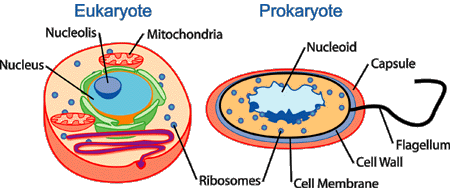
\includegraphics[width=0.6\linewidth]{images/Celltypes.png}
    \caption[Schéma cellules eucaryotes et procaryotes]{Schéma représentant une cellule eucaryote (à gauche) et une cellule procaryote (à droite). La cellule eucaryote est identifiable par un noyau entouré d'une membrane (\textit{Nucleus}), ainsi que par la présence de mitochondries, de petits organites responsables de fournir de l'énergie chimique à la cellule. En revanche, dans la cellule procaryote, le matériel génétique (nucléoïde) est librement dispersé dans le cytoplasme, sans être isolé par une membrane. Crédit image : Creative Commons.}
    \label{fig:cell_types}
\end{figure}

Le développement de la biologie moléculaire a permis d'affiner et de corriger les classifications précédentes en analysant la physiologie et la biochimie des cellules procaryotes, ainsi que les séquences d'ADN des génomes. C'est notamment en étudiant les gènes codant l'ARN 16S, que Carl Woese mis en évidence en 1977, que l'ensemble des procaryotes ne formait pas un groupe monophylétique, mais qu'ils étaient séparés en deux domaines, Bactérie et Archée \cite{woese_phylogenetic_1977}. Longtemps considéré comme des bactéries extrémophiles, il est aujourd'hui clair que les archées représentent un domaine à part entière avec toute sa singularité, comme la composition de leur membrane par exemple \cite{albers_archaeal_2011}. Malgré toute la fascination que nous pouvons avoir pour les archées, et que toutes les méthodes qui seront présentées peuvent s'appliquer aux espèces Archée, nous ne présenterons que très peu de résultats les concernant. C'est pourquoi dans la suite, même si nous parlerons de procaryote, nous considérerons plutôt les bactéries avec un prolongement possible aux archées.

\section{Taxonomie des procaryotes : un problème non résolu ?}

La classification des procaryotes et la définition d'espèce procaryote ne fait pas consensus dans la communauté des microbiologistes. Toutefois, les méthodes de classification se basent sur le même principe de relation entre les individus \cite{aldhebiani_species_2018}. Ces relations peuvent être soit phénétiques, \textit{i.e.}, reposant sur la similarité d'un trait, sans s'intéresser au lien évolutif qui pourrait les relier, soit phylogénétiques, \textit{i.e.}, reposant sur l'hérédité du caractère indépendamment de son état actuel.

Les premières tentatives de classification des bactéries reposaient sur des approches phénétiques, utilisant des critères basés sur les caractéristiques observables de ces organismes : morphologie, physiologie et biochimie.
D'un point de vue morphologique, les microbiologistes examinaient des paramètres tels que la taille des cellules, leur mode de croissance et leur capacité à former des agrégats spécifiques (\autoref{fig:morpho}). La présence ou l'absence de structures spécialisées, telles que les flagelles, était également un critère de différenciation. 
Les caractéristiques physiologiques permettaient, quant à elles, de classer les bactéries selon leur mode de vie, leurs mécanismes métaboliques (anabolisme et catabolisme) et leurs réponses aux conditions environnementales.
L'étude de la composition cellulaire offrait par ailleurs de nouveaux outils pour affiner ces classifications sur le plan biochimique. Par exemple, la coloration de Gram, méthode emblématique, permet de différencier les bactéries en deux grands groupes : les Gram-positives, caractérisées par une paroi épaisse de peptidoglycane, et les Gram-négatives, qui présentent une paroi plus fine associée à une membrane externe lipidique.
Enfin, selon le contexte d’étude, d'autres critères peuvent être intégrés. Dans le domaine médical, la pathogénicité (capacité à induire une maladie) et le sérogroupage (basé sur la composition antigénique de la capsule bactérienne) sont particulièrement utilisés pour identifier et classifier les bactéries d'intérêt clinique.

\begin{figure}[htbp]
    \centering
    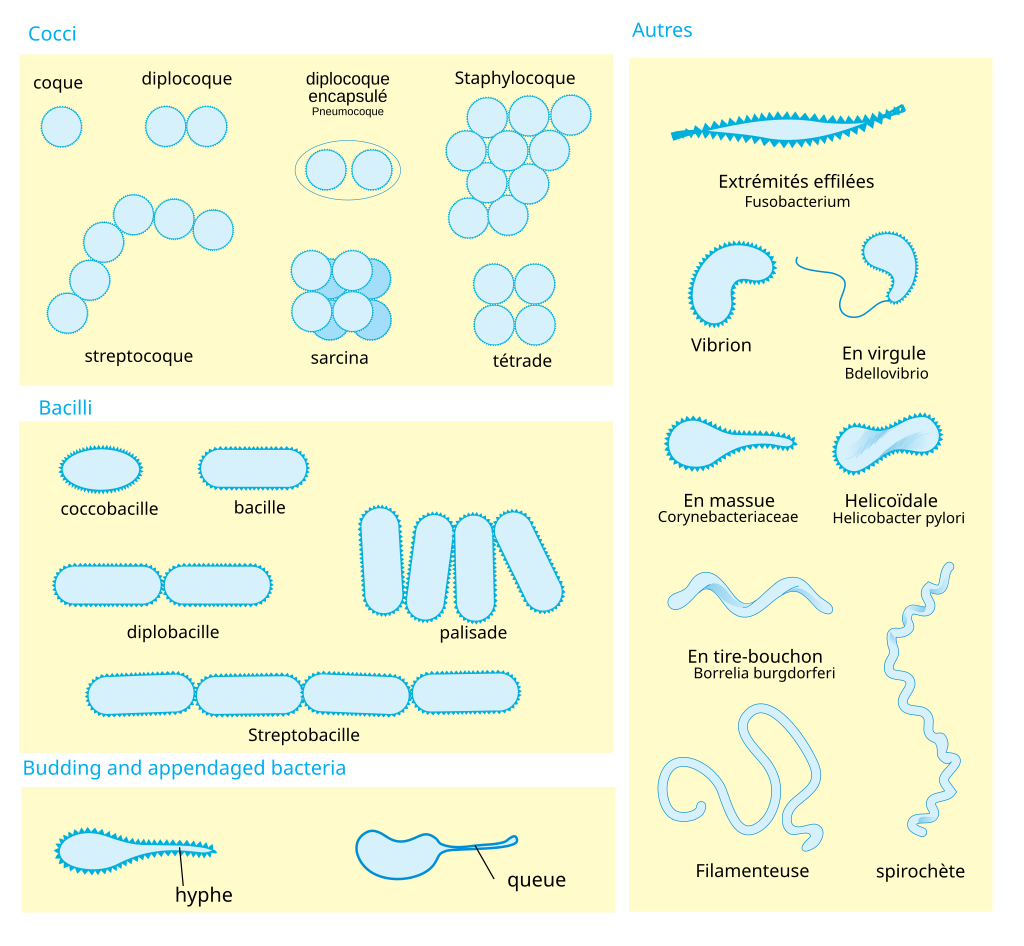
\includegraphics[width=0.75\textwidth, keepaspectratio]{images/Bacterial_morphology_diagram-fr.png}
    \caption[Morphologie et arrangement cellulaire procaryote]{Diversité morphologique des cellules procaryotes et leur arrangement. Par Mariana Ruiz Villarreal \url{https://commons.wikimedia.org/w/index.php?curid=9908634}}
    \label{fig:morpho}
\end{figure}

Avec l'arrivée de la génomique, du séquençage et de la bioinformatique, ces classifications ont peu à peu laissé leur place à des classifications basées sur la phylogénie. Néanmoins, l'ADN a aussi été utilisé comme un critère phénétique définissant des critères biochimiques comme similarité entre les souches. 
Dans ces critères, il y a d'abord le pourcentage de guanine-cytosine (GC) qui permet de différencier 2 souches appartenant à 2 genres différents si elles possèdent plus de 10 mol \%\footnote{1 équivalent molaire équivaut à 100 \% en mole, donc 10 \% en mole équivaut à 0,1 équivalent molaire.}, mais il faut noter qu'une composition en GC proche n'implique pas forcément que les souches soient proches. 
Une approche visant à définir formellement une espèce procaryote a été adoptée en 1987 par un comité d'expert \cite{moore_report_1987}. Il propose que des souches appartiennent à une même espèce si l'ADN s'hybride\footnote{Appariement de 2 brins d'ADN par complémentarité des bases} a plus de 70 \% et que le $\Delta T_m$\footnote{température à laquelle la moitié de l'ADN est dénaturés} diffère de 5 degrés ou moins.

Toutes ces approches ont permis de classer les procaryotes en taxons et dans la nomenclature actuelle, il reste des traces de ces méthodes. Elles sont d'ailleurs toujours utilisées et font partie des traits visibles dans les classifications. Il faut d'ailleurs souligner qu'il n'est pas toujours possible d'obtenir des génomes de bonne qualité pour réaliser des phylogénies.

\section{Espèce procaryote : génomique et phylogénie peuvent-elles trancher ?}

Les approches phénétiques présentées précédemment ont l'intérêt de s'appliquer au laboratoire et donc de regrouper et d'identifier les souches directement. Néanmoins, elles restent relativement approximatives et sont parfois coûteuses (en temps et en moyens). De plus, même si elles répondent aux problèmes de la taxonomie, et donc de ranger les bactéries dans des taxons, elles ne répondent pas à la question du lien entre les différents taxons et comment représenter ce lien, \textit{i.e.}, à la question de la systématique. 

Pour pallier les limites des approches précédentes, une nouvelle méthode a été développée et reste encore largement utilisée en routine aujourd'hui : la comparaison des souches à partir d'un gène marqueur. Il s'agit d'un gène présentant des variations spécifiques parmi les différentes souches d'intérêt, toutes dérivant d'une forme ancestrale commune ayant évolué différemment au fil du temps. Ainsi, le gène marqueur reflète à la fois la similarité entre les souches, permettant leur regroupement, et les événements dits de spéciation ayant conduit à leur séparation en espèces distinctes. On va privilégier l'utilisation de gènes hautement exprimés qui assurent une fonction essentielle à la vie de l'organisme : les gènes de ménage (\textit{house-keeping genes}). Un gène marqueur en particulier est utilisé : l'ADNr 16S, qui a la particularité d'être présent chez tous les procaryotes. En 2007, un arbre du vivant de toutes les espèces a été reconstruit à partir d'un arbre d'ADNr 16S comprenant toutes les souches types séquencées d'espèces de bactéries et d'archées publiées jusqu'à la fin de l'année 2007 \cite{yarza_all-species_2008}. 
En allant encore plus loin, des analyses \textit{multilocus sequence analysis} MLSA ont été proposées \cite{glaeser_multilocus_2015}. Ces analyses prennent en compte plusieurs gènes marqueurs pour réaliser la taxonomie. L'utilisation de plusieurs gènes augmente le niveau d'information et réduit les biais. Toutefois, il n'y a pas de recommandation universelle pour réaliser l'analyse et chaque MLSA est réalisé en fonction des souches de départ. La sélection des gènes et leur nombre sont des paramètres qui ont un impact encore peu évalué sur la taxonomie. Il en va de même pour la taille des fragments considérés pour chaque gène, qui ne représente qu'une partie de la séquence du gène. Enfin, expérimentalement, il est souvent difficile, voire impossible, de concevoir des amorces facilitant l'amplification des gènes dans toutes les souches prises en compte. Malgré ces critiques, l'utilisation de gènes marqueurs est encore aujourd'hui utilisée, mais est peu à peu remplacée par des méthodes prenant en compte l'ensemble du génome.

Le développement des techniques de séquençage d'ADN, initié par F. Sanger en 1977 et sa méthode éponyme \cite{sanger_dna_1977}, ont permis de séquencer les premiers génomes\footnote{le premier génome séquencé est celui du virus de bactérie MS2 \cite{fiers_complete_1976}}. Le premier génome complet procaryote (aussi le premier génome complet d'un organisme cellulaire), celui de la bactérie \textit{Haemophilus influenza}\footnote{Bactérie pathogène, responsable de maladie respiratoire ou de méningites et bactériémie.}, est séquencé en 1995 \cite{fleischmann_whole-genome_1995}. Au début des années 2000 et avec les nombreux projets autour du séquençage et de l'analyse des génomes, comme le projet génome humain \cite{lander_initial_2001}, les technologies de séquençage sont de plus en plus précises et de moins en moins coûteuses, amenant dans la génomique "moderne" : une augmentation exponentielle du nombre de séquences et des séquences plus longues et de meilleure qualité \cite{hugenholtz_prokaryotic_2021,hu_next-generation_2021}. C'est l'arrivée du \textit{Whole Genome Sequencing} (WGS) et de l'analyse de génomes complets de procaryote. Bien que les technologies de séquençage progressent, il faut aussi que les technologies et les algorithmes bioinformatiques se développent à leur tour (vitesse de calcul, gestion des données\dots), pour les utiliser en génomique comparée et en phylogénie, c'est pourquoi les méthodes présentées précédemment étaient privilégiées.

Grâce aux nouvelles méthodes de génomique comparée, que nous présenterons dans le \autoref{chap:comp}, il est désormais possible de considérer le génome complet dans les approches d'assignation taxonomique d'organismes. Une de ces approches est l'\textit{Average Nucleotide Identity} (ANI), qui rend compte de la similarité entre 2 séquences nucléotidiques. Le score d'ANI va d'ailleurs remplacer celui de l'hybridation, où un ANI inférieur 95 \% permet de différencier les espèces à la place d'une hybridation à 70 \% \cite{goris_dnadna_2007}. Plus récemment, le seuil de 95 \% a été confirmé par les auteurs de FastANI \cite{jain_high_2018}, utilisant plus de 90 000 génomes. Ils ont montré l'existence d'un \textit{gap}, espace où l'ANI diminue fortement avant 95 \% (\autoref{fig:ANI_gap_sp}).


\begin{figure}[htbp]
    \centering
    % Première image
    \subfloat{%
        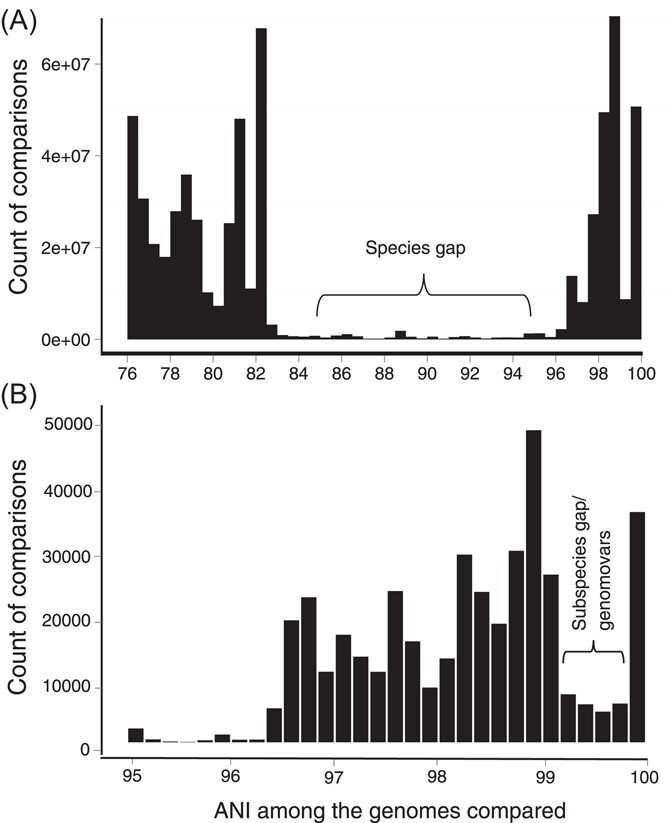
\includegraphics[width=0.5\textwidth]{images/ANI_gap.jpg}
    }
    \hfill % Espace flexible entre les deux images
    % Deuxième image
    \subfloat{%
        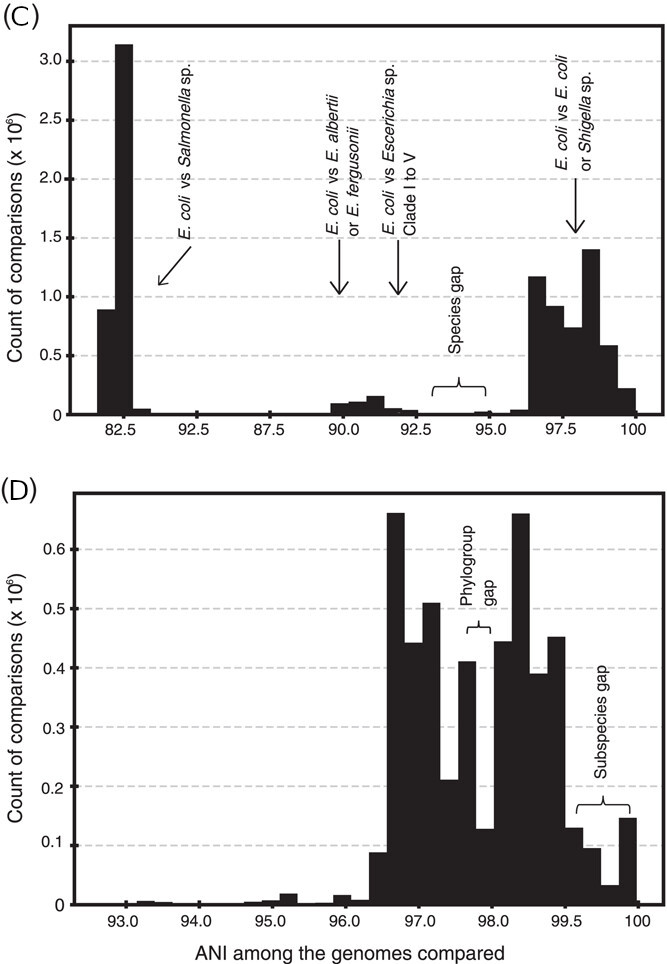
\includegraphics[width=0.44\textwidth]{images/ANI_sp.jpg}
    }
    \caption[Variation du score d'ANI au niveau de l'espèce]{Variation du score d'ANI au niveau de l'espèce. (A-B) Les histogrammes sont basés sur des comparaisons par paire effectuées avec FastANI. (A) Le Score d'ANI représenté au niveau de l'espèce se base sur les données de Jain \textit{et al}. On y retrouve un \textit{gap} entre 84 et 95 \% d'ANI. (B) Score d'ANI représenté au niveau intra-espèce sur les données de Rodrigues-R \textit{et al}. On retrouve un \textit{gap} entre 99,2 et 99,8 \% d'ANI. (C-D) Score d'ANI au niveau du groupe \textit{Escherichia coli}. Le nombre de génomes utilisés est le suivant : \textit{E. coli} : 2815 ; \textit{Salmonella enterica} : 1351 ; \textit{Escherichia fergusonii} : 57 ; \textit{Escherichia albertii} : 70 ; et \textit{Shigella flexneri} : 93 (tous les génomes complets disponibles au NCBI en juillet 2023). (C) Comparaison de l'ANI entre \textit{E.Coli} et d'autres espèces. Le seuil de 95 \% délimitant l'espèce est retrouvé. Un \textit{gap} à 97 \% existe entre \textit{E.coli} et \textit{Shigella flexneri} (une espèce d'\textit{E.Coli} particulière pour ces propriétés infectieuse). (D) Analyse de l'ANI au sein des génomes de \textit{E.Coli}. L'écart d'ANI de 99,5 \% est aussi prononcé, par rapport aux barres adjacentes, que l'écart d'ANI de 98 \%-97 \% qui correspond à l'écart entre les phylogroupes d'\textit{E. coli}, un groupe distinct et bien reconnu au sein d'\textit{E. coli}. Figures et légende adaptées de \cite{konstantinidis_sequence-discrete_2023}}
    \label{fig:ANI_gap_sp}
\end{figure}


Pourtant, la communauté n'est toujours pas arrivée à un consensus sur la classification des procaryotes en espèces et même sur l'existence d'espèces procaryotes. On peut d'abord critiquer l'approche et les résultats des études utilisant l'ANI, qui se limitent aux génomes de bonne qualité et complets, ce qui \textit{de facto} limite le nombre de génomes et d'espèces potentielles pris en compte, tout en augmentant la redondance et limitant la diversité et la variabilité. De plus, la démarche apporte le biais d'utiliser une taxonomie déjà existante. Il faut aussi prendre en compte que la dynamique évolutive des procaryotes, que nous détaillerons dans le chapitre suivant (\autoref{sec:dyn_evo}), n'est pas linéaire et héréditaire, mais que les procaryotes sont capables de recevoir et d'échanger de l'ADN. C'est pourquoi des auteurs soutiennent une définition plus écologique de l'espèce procaryote \cite{luo_genome_2011}, prenant en compte ces échanges agissant sur la \textit{fitness} des organismes dans leur environnement.


On peut donc convenir qu'il n'est pas encore communément admis de parler d'espèce procaryote. Il existe toutefois des caractéristiques communes et spécifiques aux procaryotes ainsi que des traits propres à chaque taxon. De nombreuses méthodes et démarches scientifiques parviennent à construire une phylogénie des procaryotes, mais celle-ci doit être replacée dans son contexte d'étude pour prendre sens. Notamment dans les travaux de recherches que j'ai réalisés, où il était nécessaire de se baser sur une classification des génomes en espèce. Dans le contexte de nos travaux, la similarité des séquences l'emporte comme critère de classification, nous utiliserons donc des génomes provenant de bases de données utilisant des critères comme l'ANI ou des gènes marqueurs pour construire des pangénomes.

%Enfin, avec l'explosion du nombre de séquences disponible, nous voyons l'émergence d'un paradoxe : de plus en plus de données sont disponibles, mais alors que l'on pensait pouvoir ranger les procaryotes dans des boites bien précises qui se verraient valider au cours du temps, une nouvelle exception vient renverser l'ordre actuel et la phylogénie doit être revue.

\section{Systématique : l'homologie et ses déclinaisons}

Les méthodes présentées ci-dessus, sont  des aides précieuses pour convenir d'une taxonomie des procaryotes, mais aussi pour étudier leur évolution au cours du temps et retracer l'origine et l'histoire des gènes. Il reste donc à lier et à représenter le lien entre les gènes. 

Une première approche intuitive est de rechercher une origine commune entre les gènes, appelé gène ancestral. Si un tel gène existe, on dit que les gènes issus de ce gène ancestral sont homologues. Dans un second temps, il convient d'étudier les évènements évolutifs qui ont conduit à la séparation des gènes pour préciser le type d'homologie (\autoref{fig:homologue}). 
Le premier évènement est un évènement dit de spéciation et conduit à l'émergence d'une espèce. Dans ce cas, si les gènes sont uniquement séparés par des spéciations, on dit qu'ils sont orthologues. Le second évènement est une duplication des gènes sur le même génome (cf. \autoref{sec:rearragement}). Les gènes sont alors dits paralogues et vont évoluer de façon indépendante dans le génome. Un autre évènement évolutif, fréquent chez les procaryotes, est celui du transfert horizontal, \textit{i.e.}, l'échange de matériel génétique entre organismes (cf. \autoref{sec:evo_hz}). Lorsque des gènes sont transférés horizontalement, ils sont dits xenologue.

\begin{figure}[htbp]
    \centering
    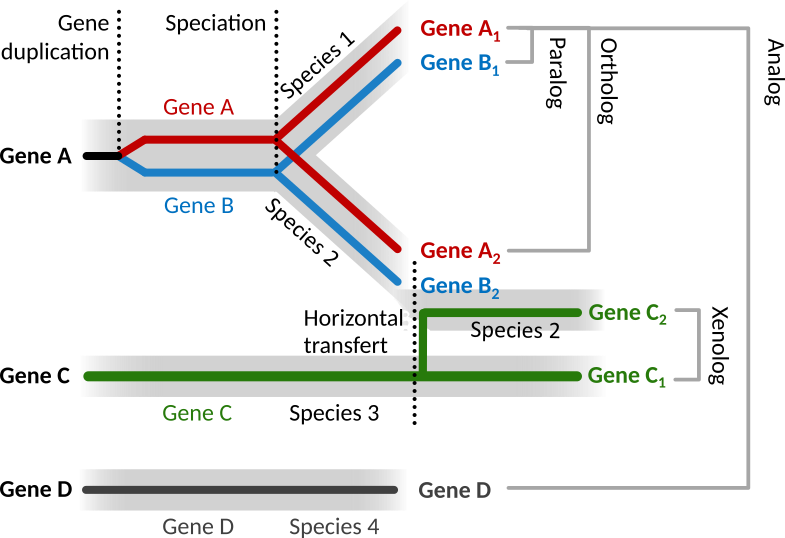
\includegraphics[width=.9\textwidth]{images/homologs.png}
    \caption[Schéma représentatif des différents types d'homologie]{Schéma représentatif des différents types d'homologie. Figure extraite et adaptée de \url{https://en.m.wikipedia.org/wiki/Sequence_homology} sous licence Creative Common}
    \label{fig:homologue}
\end{figure}

Toutes ces notions sont essentielles pour poser des hypothèses de travail qui seront utilisées dans les analyses de génomique comparée \cite{koonin_orthologs_2005,stamboulian_ortholog_2020}. Une de ces hypothèses que nous utiliserons dans nos analyses est celle que des gènes homologues vont coder pour des fonctions similaires\footnote{\textit{N.B} : 2 gènes codant pour la même fonction ne sont pas nécessairement homologues. Il existe des cas de convergence évolutive, \textit{i.e.}, une fonction similaire sans origine commune. Il est aussi possible que des séquences courtes ou peu complexe semble homologue, mais cette apparente homologie serait liée au hasard.}. Plus précisément, on suppose que des gènes orthologues vont coder pour une même fonction et vont donc faire également partie du même processus. Les gènes paralogues peuvent avoir des fonctions différentes, mais qui reste proche, par exemple pour des enzymes, le substrat va changer, mais la réaction rendra un produit chimiquement proche \cite{mirny_using_2002}.
\chapter{Génomique des procaryotes : organisation, évolution et fonctions}

Les génomes procaryotes sont souvent décrits comme plus simples et plus faciles à étudier que les génomes eucaryotes. La simplicité apparente de ces génomes cache en réalité des mécanismes complexes. Dans cette partie, je décrirai les mécanismes les plus connus et les plus répandus.

\section{Structure et organisation des génomes procaryotes}
\label{sec:structure_org}

%Le génome correspond à l'ensemble du matériel génétique, c.-à-d., des éléments qui seront hérités par les cellules de la génération suivante. Le génome, c'est aussi la structure de base qui va contenir l'ensemble des informations nécessaires au fonctionnement et à la survie de la cellule. Ces informations sont contenues dans la molécule d'ADN, ce qui nous amène à la structure primaire du génome, la séquence nucléotidique. Cette séquence est souvent circulaire chez les procaryotes et est de petite taille, quelques centaines de milliers de bases, mais certains génomes peuvent atteindre plusieurs millions de bases\footnote{En bioinformatique, on utilise l'unité base (b) ou paire de base (pb), pour mesurer la taille d'un génome. Un génome procaryote sera donc compris entre 100 kb et 10 Mb. Pour comparaison, le génome humain mesure environs 3 Gb.} (\autoref{fig:genome_size}).

Le génome procaryote correspond à la séquence de nucléotides qui composent la molécule d'ADN qui est bicaténaire, \textit{i.e.}, composée de deux brins antiparallèles reliés par complémentarité des bases (A$\leftrightarrow$T, C$\leftrightarrow$G). Le génome est souvent circulaire et de petite taille, quelques centaines de milliers de bases, mais certains génomes peuvent atteindre plusieurs millions de bases\footnote{En bioinformatique, on utilise l'unité base (b) ou paire de base (pb), pour mesurer la taille d'un génome. Un génome procaryote sera donc compris entre 100 kb et 15 Mb. Pour comparaison, le génome humain mesure environs 3 Gb.} (\autoref{fig:genome_size}). Enfin, le génome se divise en deux grandes catégories : l'ADN codant et l'ADN non codant.

\begin{figure}[htbp]
    \centering
    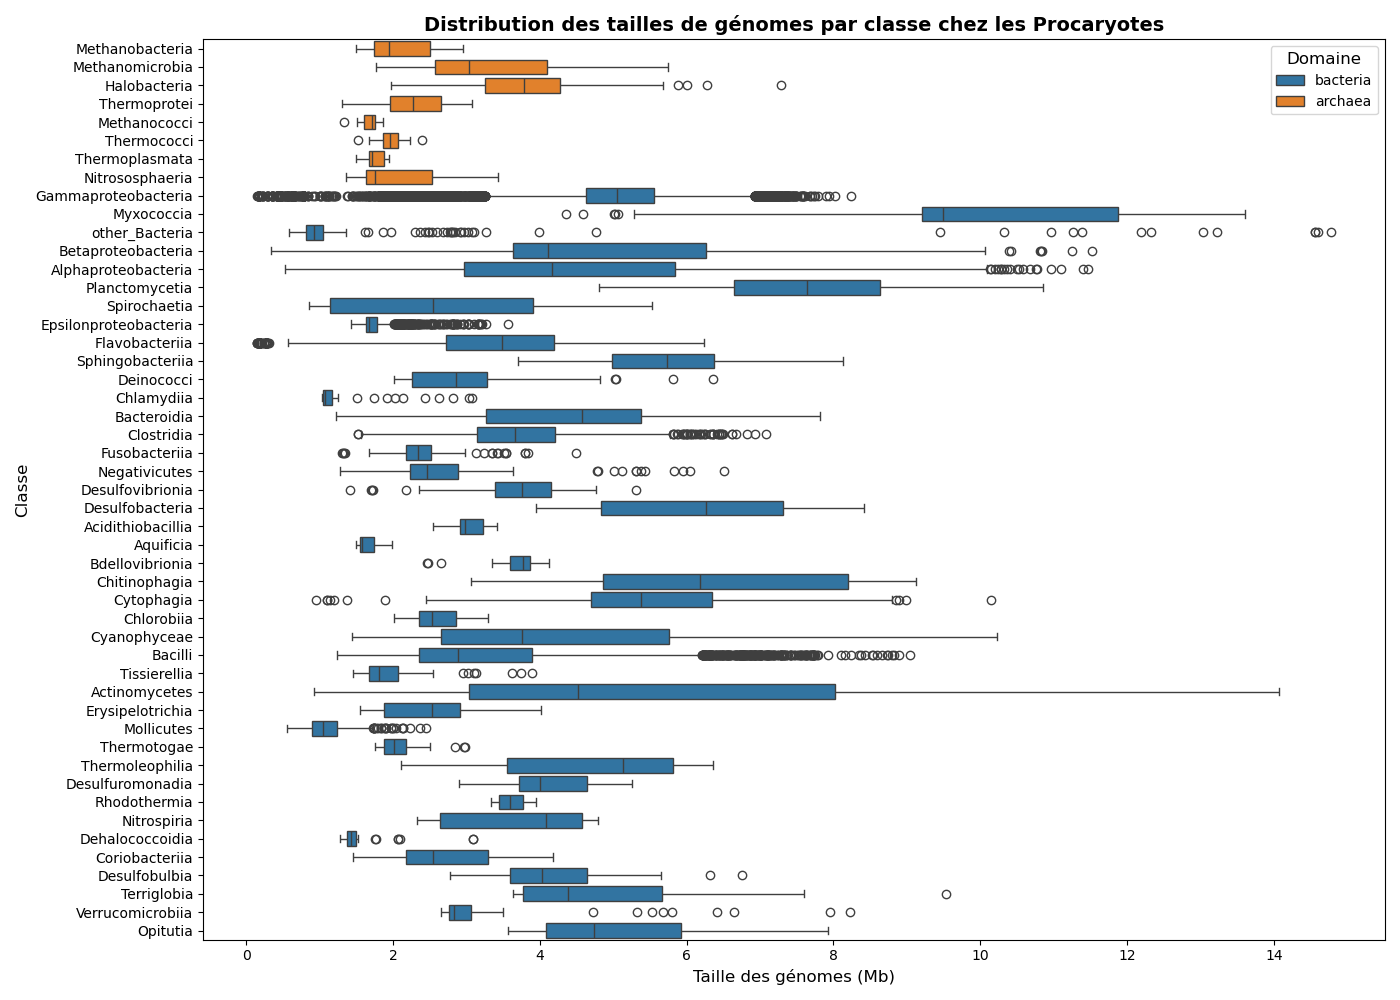
\includegraphics[width=\textwidth]{images/genome_sizes_boxplot.png}
    \caption[Distribution de la taille des génomes chez les procaryotes]{Distribution de la taille des génomes (en base) par classe chez les procaryotes. Les données utilisées proviennent de RefSeq version 28 janvier 2025.}
    \label{fig:genome_size}
\end{figure}

\newpage
\subsection{Constituant du génome : le codant et le non codant}
\label{sec:gene}
%\subsection{Organisation génique des procaryotes}
Chez les procaryotes, le génome est majoritairement constitué de séquences codantes (entre 85 et 90 \%), ce qui compense leur petite taille. 
L'ADN codant correspond à des blocs de nucléotides d’environ 1 kb. Ces blocs codants sont appelés gènes et ils jouent un rôle essentiel puisqu’ils contiennent l’information nécessaire à la production des protéines impliquées dans toutes les réactions cellulaires (cf. \autoref{sec:fn_reg}). De plus, l’ADN procaryote étant bicaténaire, chaque gène peut alors être lu dans les deux directions (sur le brin direct ou complémentaire), doublant ainsi la quantité d'information sur une position précise du génome (locus). 

Dans le génome, les gènes ne sont pas répartis aléatoirement. Ceux qui codent une fonction biologique similaire sont souvent regroupés dans un  contexte génomique. La conservation de l'ordre des gènes, appelé aussi synténie, peut varier entre les génomes, mais les gènes restent dans le même contexte \cite{lathe_gene_2000}, on parle alors de contexte conservé ou de synténie conservée. De plus, la position des gènes par rapport à l'origine de réplication (Ori: région où commence la réplication de l'ADN) à aussi son importance. Il a été montré que chez les bactéries avec un fort taux de division, les gènes ayant un rôle essentiel sont plus proches de l'Ori afin d'être plus fortement exprimés \cite{sharp_chromosomal_1989,vieira-silva_systemic_2010}.
%Les gènes sont soumis à des mécanismes de régulation communs (cf. \autoref{sec:fn_reg}).

Pour finir, les gènes peuvent être classés selon l’importance de leur fonction pour la survie de la cellule. Les gènes indispensables au cycle de vie d'une cellule, par exemple la réplication de l’ADN, la transcription, ou la traduction, sont dits "essentiel" et se distinguent des gènes "accessoires", qui codent pour des fonctions d'adaptation à des conditions particulières, comme la résistance aux antibiotiques, la défense contre les virus ou des transformations métaboliques spécifiques.



%Le génome est divisé en sous-unité que l'on appelle gène. Le gène contient l'information nécessaire pour produire une protéine qui réalisera une fonction dans la cellule (\autoref{fig:gene2prod}), on dit que le gène code pour une protéine. Pour ça, l'ADN est d'abord transcrit en une molécule d'ARNm, qui sera traduite en protéine (gène A sur la \autoref{fig:genome_size}) par des complexes protéine/ARN, les ribosomes. Ces protéines correspondent à une chaîne d'acides aminés, que l'on peut représenter sous forme de séquence. Pour passer d'un gène à une protéine, on utilise une table de correspondance que l'on appelle code génétique où 3 nucléotides correspondent à 1 acide aminé. En moyenne, une protéine contient 300 acides aminés, ramenant la taille des gènes à environ 1 kb. Enfin, comme indiqué sur la partie haute de la \autoref{fig:genome_size}, les génomes procaryotes sont majoritairement codants, ce qui veut dire que presque tout l'ADN peut être divisé en gènes, et donc qu'il y a environ entre 100 et 10 000 gènes dans les génomes en fonction de leur taille. En mettant toutes ces informations en perspective, on comprend que la petite taille des génomes procaryotes est compensée par son fort taux de gènes, et qu'ainsi, il contient l'ensemble des protéines nécessaires à la survie de la cellule. 


\begin{figure}[htbp]
    \centering
    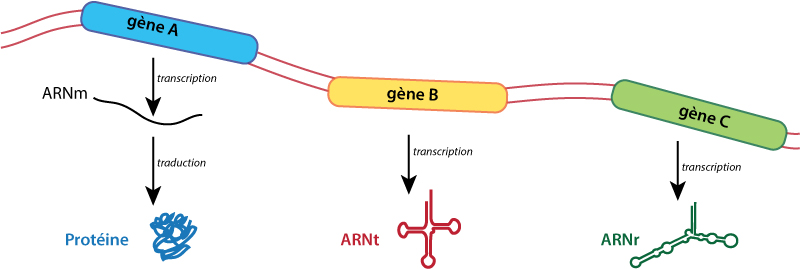
\includegraphics[width=\linewidth]{images/gene2prot.jpg}
    \caption[Produit d'un gène]{Produit d'un gène dans la cellule. Un gène est d'abord transcrit en ARN. Si l'ARN transcrit est dit messager (ARNm), il sera ensuite traduit en protéine, sinon l'ARN produit (ARNt, ARNr, miARN, ....) aura un rôle spécifique dans des processus cellulaire. Copié de RNBio, Sorbonne université. \url{https://rnbio.sorbonne-universite.fr/genetique_genotype1}}
    \label{fig:gene2prod}
\end{figure}

L'ADN non codant constitue une part tout de même importante du génome et selon l'adage "la nature a horreur du vide"\footnote{Citation d'Aristote qui, répondant à Démocrite, dit que l'univers ne pouvait être rempli de vide. On sait aujourd'hui que Démocrite avait raison, mais dans le cas des génomes procaryote, l'idée fonctionne.}. Cet ADN non codant, n'est donc pas inutile et renferme également des fonctions essentielles à la vie de la cellule.
Tout d'abord, on retrouve les séquences d'ADN qui seront transcrits en ARN ribosomiques (ARNr) ou ARN de transfert (ARNt). Ces ARN sont indispensables pour la construction de la chaîne d'acide aminée de la protéine. Ces séquences d'ADN sont considérée aussi comme des gènes et selon les sources comme faisant partie du codant. Cependant, d'un point de vue sémantique et biologique ces gènes ne code pas, les nucléotides sont copiés d'une forme d'acide désoxyribonucléique en une forme d'acide ribonucléique. L'ADN non codant renferme d'autres formes d'ARN, comme les microARN et les ARN interférents (miARN et siARN). Ces ARN sont aujourd'hui considérés comme des acteurs clés dans la régulation des fonctions biologiques \cite{backofen_bioinformatics_2014,watkins_regulatory_2019}, mais aussi dans d'autres processus comme le système immunitaire \cite{bobadilla_ugarte_argonaute_2023}.

L'ADN non codant n'a pas uniquement le rôle de contenir les séquences transcrites en ARN, il contient aussi d'autres éléments régulateurs de l'expression des gènes contenus dans l'espace intergénique (cf. \autoref{sec:fn_reg}). On retrouve aussi dans l'ADN non codant des séquences répétées, comme les séquences d'insertion (IS) qui se déplace dans le génome, ou les séquence CRISPR (Régions composées de répétitions palindromiques et d’espacers, impliquées dans le système immunitaire adaptatif des bactéries) \cite{jansen_identification_2002,bolotin_clustered_2005}. Il existe tout de même une partie d'ADN non codant qui n'a aucun rôle, ces séquences sont des vestiges d'anciens gènes qui au cours de l'évolution ont perdu leur fonction (cf. \autoref{sec:dyn_evo}). Pour terminer, c'est aussi dans le non-codant que l'on va retrouver des éléments essentiels dans la réplication et l'évolution des génomes procaryotes : l'origine de réplication (Ori) et les éléments génétique mobile (MGE). 
%Tous les gènes ne sont pas traduits en protéine, une partie de ces gènes seront transcrit dans des formes d'ARN ayant un rôle dans la régulation et le fonctionnement de la cellule. Les ARN ribosomiques (ARNr), sont les constituants fondamentaux de la structure et du fonctionnement des ribosomes. Ils vont interagir avec les ARN de transfert (ARNt), qui acheminent les acides aminés vers les ribosomes pour traduire l'ARNm en protéine. D'autres ARN, comme les microARN et les ARN interférents (miARN et siARN), interviennent dans la régulation de l'expression des gènes. Cette liste non exhaustive montre la diversité des ARN et beaucoup étaient encore considérés il y a peu comme des produits secondaires sans réelle fonction. Aujourd'hui, ils sont considérés comme des acteurs clés dans la régulation des fonctions biologiques \cite{watkins_regulatory_2019,backofen_bioinformatics_2014}, mais aussi dans d'autres processus comme le système immunitaire \cite{bobadilla_ugarte_argonaute_2023}

\subsection{Réplicons et mécanismes de réplication dans les génomes procaryotes}
\label{sec:replicons}
La multiplication des cellules procaryotes s'effectue par division, où une cellule mère donne naissance à deux cellules filles. Afin de transmettre l’information génétique aux cellules nouvellement formées, l’ADN doit être répliqué, \textit{i.e.}, copié de manière exacte. Le terme réplicon désigne l’ensemble des molécules d’ADN capables de se répliquer de façon autonome. Un réplicon contient ainsi tous les éléments nécessaires à l’exécution et à la régulation de la réplication. Chaque réplicon contient une séquence d’ADN spécifique, appelée origine de réplication (Ori), où commence le processus de réplication.

La forme principale de réplicon dans la cellule procaryote est le chromosome. Le chromosome, souvent circulaire et replié, constitue le plus grand réplicon en termes de paires de bases. Chez les procaryotes, le chromosome est généralement unique, bien que d'autres réplicons puissent coexister au sein de la cellule.

Une seconde forme de réplicon, connue pour son rôle dans l’évolution (voir \autoref{sec:evo_hz}), est le plasmide \cite{lederberg_gene_1946,lederberg_sex_1953}. Les plasmides, souvent circulaires et de taille inférieure à celle du chromosome, sont indépendants de ce dernier. En tant que réplicons, ils se répliquent de manière autonome et peuvent être présents en grand nombre dans une cellule. L’origine de réplication des plasmides diffère de celle des chromosomes. Par ailleurs, les plasmides peuvent accumuler de nouvelles séquences et augmenter en taille, prenant alors la forme de mégaplasmides (\autoref{fig:replicon}).

Chez la majorité des procaryotes, le chromosome contient les gènes essentiels, tandis que les plasmides portent des gènes accessoires. Cependant, certaines formes de réplicons oscillent entre chromosome et plasmide. Par exemple, chez \textit{Rhodobacter sphaeroides}\footnote{Bactérie présente dans les lacs profonds et les eaux stagnants. Elle est capable de réaliser la photosynthèse et son métaolisme est très diversifié et donc très utilisé en biotechnologie} et \textit{Vibrio cholerae}\footnote{Bactérie responsable du choléra, on la retrouve dans l'eau et peut se propager entre humain en utilisant la transpiration}, un second chromosome a été identifié \cite{suwanto_physical_1989,trucksis_vibrio_1998}. Aujourd'hui, ces chromosomes secondaires sont distingués d'une forme de réplicons proche, le chromide \cite{harrison_introducing_2010}. Les chromides, de taille intermédiaire entre un plasmide et un chromosome principal, contiennent des gènes essentiels à la cellule. Ces gènes présentent une proximité phylogénétique avec les espèces du même genre, contrairement à ceux du chromosome principal, qui sont conservés au-delà du genre. En revanche, en termes de mécanismes de réplication et de séquences Ori, les chromids utilisent des systèmes de type plasmidique.

L’usage des termes chromosome secondaire, chromid et mégaplasmide demeure actuellement peu standardisé dans la littérature \cite{hall_what_2021}. Plusieurs critères permettent néanmoins de les distinguer. Le premier repose sur le contenu génétique : les mégaplasmides n’abritent pas de gènes essentiels, contrairement aux chromosomes secondaires et aux chromids. Le second critère est la composition en nucléotides, qui est plus proche de celle du chromosome principal pour les chromids et les chromosomes secondaires. Enfin, leur origine évolutive les différencie : le chromosome secondaire résulte de la scission d’un chromosome ancestral en un chromosome principal et un secondaire, tandis que le chromid dérive d’un ancien mégaplasmide ayant perdu sa capacité de mobilité (voir \autoref{sec:evo_hz}) et qui a intégré des gènes essentiels (\autoref{fig:replicon}). Les chromides auraient donc plutôt un rôle de réservoir de gènes d'intérêt et d'adaptation améliorant la \textit{fitness} des organismes. Cette vision vertueuse de l'accumulation de gènes s'oppose directement à la vision plus ancienne des plasmides non mobilisable décrits comme parasitant la cellule \cite{levin_accessory_1993,lili_persistence_2007}.

\begin{figure}[htbp]
    \centering
    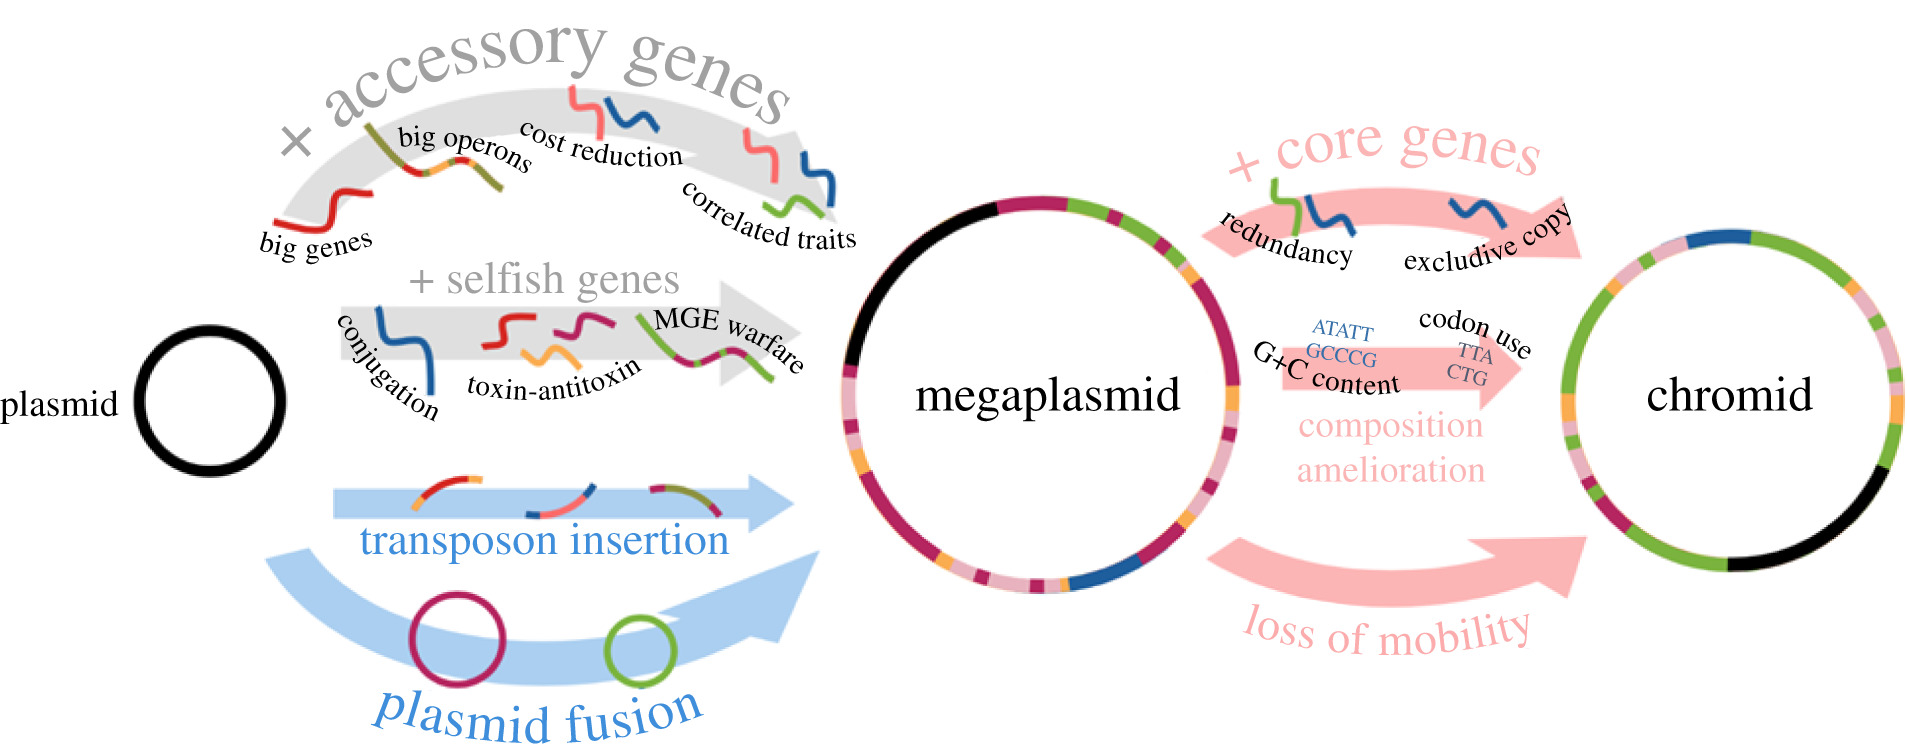
\includegraphics[width=0.8\linewidth]{images/replicon.jpg}
    \caption[Évolution d'un plasmide en chromid]{Schéma simplifié de l'évolution d'un plasmide en megaplasmide et de megaplasmide à chromid. Figure extraite de \cite{hall_what_2021}}
    \label{fig:replicon}
\end{figure}



\newpage
\section{Dynamique évolutive des génomes}
\label{sec:dyn_evo}

La dynamique évolutive des procaryotes est caractérisée par des processus continus de gain, perte et modification de gènes (\autoref{fig:dyna_evo}). La taille des génomes étant restreinte, la perte de gènes peut optimiser le génome en éliminant les séquences redondantes ou non essentielles, favorisant ainsi une efficacité accrue dans des environnements spécifiques. Les modifications génétiques, quant à elles, jouent un rôle crucial dans l'adaptation fine des procaryotes face aux pressions sélectives variées. L'acquisition de nouveaux gènes introduit une diversité génétique, pouvant conférer des traits avantageux, tels que la résistance aux antibiotiques ou la capacité à métaboliser de nouvelles sources de nutriments.

\begin{figure}[htbp]
    \centering
    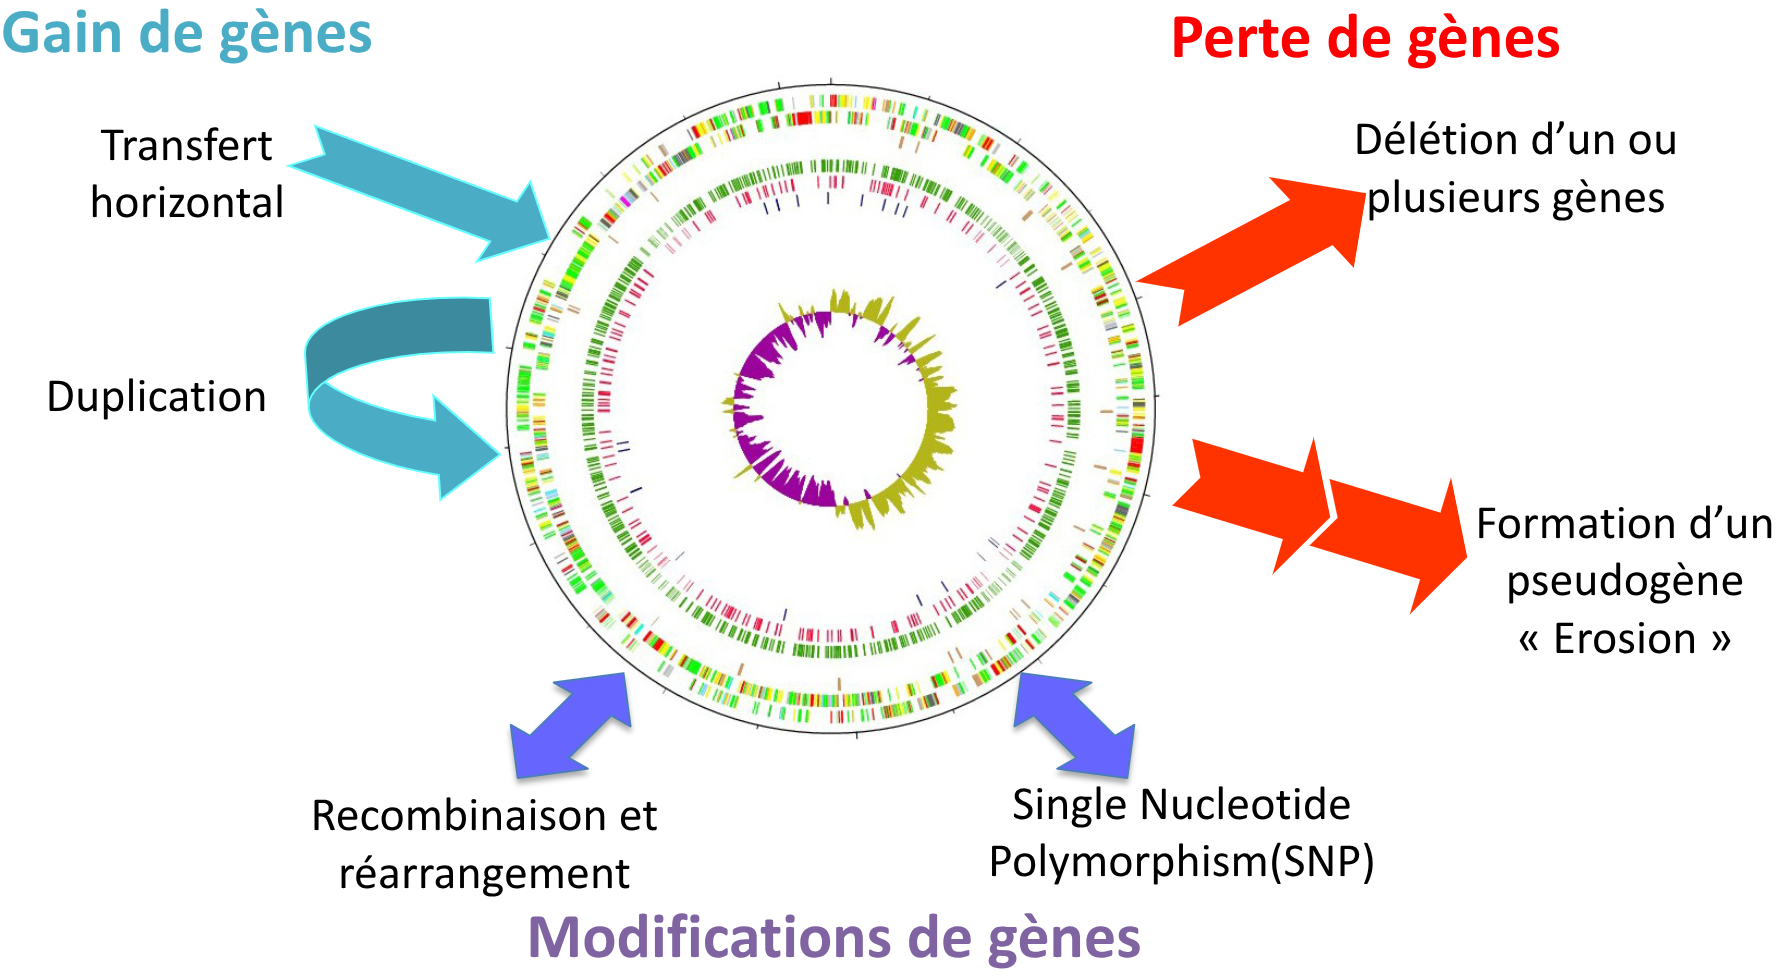
\includegraphics[width=\linewidth]{images/DynamiqueEvo.png}
    \caption[Schéma de la dynamique évolutive des génomes procaryotes]{\textbf{Schéma résumant la dynamique évolutive des génomes procaryotes.} Source LABGeM}
    \label{fig:dyna_evo}
\end{figure}

 Les gènes doivent ensuite être transmis dans la population. Les \textbf{transferts verticaux} permettent de transférer les gènes de génération en génération, assurent la continuité et la stabilité des traits essentiels. Les \textbf{transferts horizontaux} permettent l'échange de gènes entre les organismes, favorisant une diversification rapide des génomes, qui peut radicalement transformer les capacités adaptatives des lignées procaryotes. Cette dynamique complexe façonne la biodiversité procaryote et témoigne de la capacité évolutive exceptionnelle de ces organismes à coloniser une multitude d'écosystèmes.

\subsection{Mécanismes d'évolution par transfert vertical}
\label{sec:evo_ver}
Les mécanismes d'évolution par héritage regroupent les processus menant à une modification du génome entre la cellule mère et la cellule fille. Théoriquement, lors de la division cellulaire, la cellule mère se divise en 2 cellules filles possédant exactement la même information génétique qu'elle. Pourtant, malgré un ensemble de mécanismes de protection et de correction de l'ADN, le génome peut différer entre les cellules mère et fille. Ce sont ces "erreurs" qui vont nous intéresser, car ce sont elles qui sont à l'origine de l'innovation et de la diversité génétique.

\newpage

\subsubsection{Impact des mutations génétiques : SNPs, Indels et pseudogènes}
\paragraph{\textit{Single Nucleotid Polymorphism}}

Un \textit{Single Nucleotide Polymorphism} (SNP) correspond à une modification de la séquence induite par la mutation d'un nucléotide en un autre.
Étant donné que le code génétique est dégénéré\footnote{Un acide aminé peut être codé par plusieurs codons différents.}, la mutation peut ne pas avoir d'impact sur la séquence de la protéine, on dit alors que la mutation est silencieuse ou même sens. Si la modification entraîne un changement d’acide aminé dans la séquence protéique, on parle de mutation faux-sens. Enfin, une mutation est qualifiée de non-sens lorsqu'elle introduit prématurément un codon STOP, interrompant ainsi la traduction et conduisant à une perte de fonction de la protéine. Une telle mutation peut également affecter un site fonctionnel clé (comme un site actif), compromettant l’activité de la protéine. Lorsque l’introduction d’un codon STOP précoce rend un gène non fonctionnel, ce dernier devient un \textbf{pseudogène}, un vestige génomique dépourvu de rôle biologique actif, un phénomène appelé pseudogénisation.

Sur la \autoref{fig:mec_evo}, la première mutation implique un changement de glutamine en histidine, des acides aminés aux propriétés de polarité et de charge différentes. Il s’agit donc d’une mutation faux-sens, qui aura probablement un impact significatif sur la structure de la protéine. En revanche, les deux autres SNPs ne modifient pas l’acide aminé codé, ils sont donc silencieux.

\begin{figure}[htbp]
    \centering
    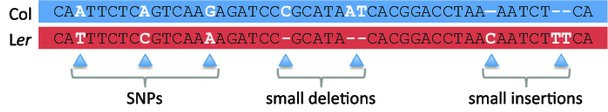
\includegraphics[width=.65\textwidth]{images/Mec_evo.jpg}
    \caption[Identification des SNP et indels entre 2 génomes]{\textbf{SNP et InDels entre deux génomes.} On suppose que le premier codon commence par le premier nucléotide. Figure extraite et adaptée de \cite{qi_detection_2014}}
    \label{fig:mec_evo}
\end{figure}

\paragraph{Indels: insertion, délétion et pseudogènes}

Un indel correspond à l'insertion (In) ou la délétion (del)\footnote{On regroupe l'insertion et la délétion, car sans une analyse phylogénétique, il est impossible de les différencier par comparaison de séquence.} d'un ou plusieurs nucléotides dans la séquence d'un gène. Lorsque la taille de l'indel est un multiple de 3 (insertion ou délétion d'un codon), la séquence protéique peut soit être allongée, soit raccourcie d'un acide aminé, soit coupée de façon précoce si le codon est un codon STOP.

Si la taille de l'indel n'est pas un multiple de 3, il y aura un décalage du cadre de lecture ou \textit{frameshift}. Ce décalage va induire un changement de tous les acides aminés de l'indel à la fin du gène, provoquant avec lui un changement dans la fonction de la protéine ou une inactivation de la fonction. La partie du gène qui n'est pas décalée est alors considérée comme un fragment du gène initial, il est alors qualifié de pseudogène. À nouveau, cette mutation peut être délétère pour la cellule. Sur la \autoref{fig:mec_evo}, les indels sont de taille 1 et 2, elles ne provoquent pas l'apparition d'un codon STOP précoce, mais l'ensemble des acides aminés est modifié.

Les indels vont donc transformer la séquence protéique traduite, pouvant nuire à la fonction de cette dernière et être délétère pour l'organisme. Pour éviter les problèmes liés aux \textit{frameshifts}, il a été montré qu'il existe un fort taux de codon STOP hors du cadre de lecture \cite{tse_natural_2010}. Cette adaptation permettrait de limiter la traduction des protéines mutantes et d'ainsi limiter le coût énergétique pour la cellule. Il a aussi été montré que les \textit{frameshifts} pourraient être à l'origine d'un réservoir d'adaptation à l'environnement \cite{koch_catastrophe_2004}. Lors d'un changement dans l'environnement créant une nouvelle pression de sélection, un \textit{frameshift} pourrait produire une protéine qui permet à l'organisme de s'adapter à son environnement et donc d'améliorer sa \textit{fitness}\footnote{Le \textit{fitness} correspond à la capacité d'un individu de survivre dans son environnement et à se reproduire}. Une fois que l'élément perturbateur de l'environnement disparaît, un nouveau \textit{frameshift} pourrait ramener le cadre de lecture à sa place d'origine. Ce mécanisme, en accord avec la petite taille des génomes, aurait l'intérêt de ne pas perdre des gènes d'adaptation à l'environnement, même s'ils ne sont nécessaires que ponctuellement.

\subsubsection{Réarrangement génomique : un moteur de l'évolution}
\label{sec:rearragement}

Les génomes évoluent également suite à des événements de réarrangement. Ils impliquent des segments d'ADN plus importants. La forme du génome obtenue, appelée variant structural (SV pour \textit{Structural variant} en anglais), est plus difficile à détecter que les SNP et les indels \cite{periwal_insights_2015}.

Le mécanisme de recombinaison est à l'origine des réarrangements. Une recombinaison implique l'échange de 2 portions d'ADN entre 2 molécules ou 2 régions d'ADN. La recombinaison peut être homologue, se produisant entre des séquences similaires, ou non-homologue, impliquant des séquences différentes. Elle est souvent médiée par des enzymes spécialisées comme RecA ou des intégrases, qui permettent l'intégration, la réparation ou le réarrangement précis des séquences. La recombinaison homologue est cruciale pour la réparation des cassures de l'ADN, les réarrangements et également dans l'acquisition de nouveaux gènes par transfert horizontal (cf. \autoref{sec:evo_hz}) \cite{eisenstark_genetic_1977}.

Les réarrangements de l'ADN correspondent donc à un échange entre 2 segments du génome, induisant une insertion, une délétion ou une modification de l'ordre des nucléotides (\autoref{fig:rearrangement}). Les réarrangements sont fréquents dans les génomes procaryotes \cite{sun_genome-wide_2012} et peuvent être spontanés ou facilités par la présence d'éléments mobiles, tels que les transposons, qui sont des séquences d'ADN capables de se déplacer au sein du génome. Ils sont composés de gènes codant pour une transposase, l'enzyme responsable de son déplacement, ainsi que de séquences répétées aux extrémités, nécessaires à la reconnaissance et à l'excision du transposon. 

L'ordre des gènes étant important dans l'expression des gènes et la fonction des protéines, le SV résultant peut conduire à une modification de l'expression génique ou à un changement dans la fonction de la protéine. Il existe 3 formes de réarrangement : symétrique, asymétrique et au sein d'un réplicon. Ces formes ne sont pas toutes équiprobables, car elles affectent plus ou moins la structure du génome. Aussi, les réarrangements proches de l'Ori sont plus fréquents que ceux proches du site de terminaison \cite{darling_dynamics_2008}. 

\begin{figure}[htbp]
    \centering
    \subfloat{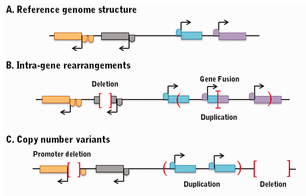
\includegraphics[width=0.5\textwidth,keepaspectratio]{images/rearrangement1.png}}
    \subfloat{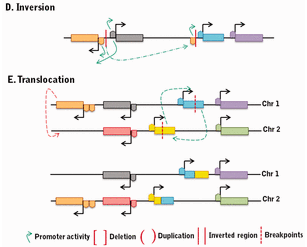
\includegraphics[width=0.4\textwidth,keepaspectratio]{images/rearrangement2.png}}
    \caption[Réarrangement et implication]{\textbf{Réarrangement et conséquences des variants structuraux.} (A) Région génomique sans SV. Les rectangles représentent les gènes et les petits connecteurs à côté représentent le promoteur du gène concerné. (B) Réarrangement intragénique illustrant la délétion et la fusion de gènes à la suite d'une duplication partielle du gène. Les régions codantes modifiées produisent des transcrits aberrants. La délétion ou la duplication peut entraîner une modification du nombre des gènes dans des régions par ailleurs fonctionnellement intactes. (C) Délétion du promoteur, la régulation est modifiée et une duplication/délétion qui modifie le nombre de copies des gènes. (D) Inversions affectant la structure du gène, le gène est inversé, retourné et réarrangé, ce qui éloigne l'un des promoteurs du premier gène (orange). (E) Translocations affectant le contexte génique. Figure extraite et adaptée de \cite{periwal_insights_2015}}
    \label{fig:rearrangement}
\end{figure}

Les recombinaisons peuvent également conduire à la duplication de gènes ou de régions génomiques, un mécanisme clé dans l’évolution des procaryotes en générant une redondance génétique. Cette redondance offre une opportunité évolutive : tandis qu’une copie du gène conserve sa fonction initiale, l’autre peut accumuler des mutations, potentiellement aboutissant à une nouvelle fonction, sans compromettre la survie de l’organisme. En outre, la duplication peut jouer un rôle dans la régulation de l’expression génique. Par exemple, les gènes codant pour les pompes à efflux, impliquées dans l’évacuation des antibiotiques hors de la cellule, sont fréquemment dupliqués, favorisant ainsi une meilleure résistance aux traitements \cite{maddamsetti_duplicated_2024}. Toutefois, les événements de duplication restent moins fréquents que les transferts horizontaux de gènes dans les génomes procaryotes \cite{tria_gene_2021}. Cette rareté s’explique en partie par les mécanismes d’élimination de la redondance, qui optimisent la compacité et l’efficacité des génomes bactériens.

Les mécanismes qui viennent d'être décrits apportent de l'innovation dans les génomes procaryotes, qui doit ensuite être transmise dans la population. Avec le transfert vertical, cette transmission se fait uniquement d'une génération à l'autre, un processus limité par le temps de génération, qui varie selon l'espèce (\textit{E. coli} : 20 min, \textit{Lactobacillus acidophilus} : 80 min, \textit{Mycobacterium tuberculosis} : 800 min). Un temps de génération plus long semble aussi réduire le taux de mutation spontanée de l'ADN \cite{weller_generation-time_2015}. Pour contourner ces contraintes, les procaryotes échangent de l’ADN avec leur environnement (autres bactéries, virus, eucaryotes, ADN libre\dots), par un ensemble de processus regroupé sous le terme de \textbf{transfert horizontal}, qui leur permet d’acquérir de nouvelles fonctions génétiques.

\subsection{Mécanismes d'évolution par transfert horizontal}
\label{sec:evo_hz}

Les transferts horizontaux de gènes (\textit{Horizontal Gene Transfert} en anglais, HGT) constituent un phénomène central dans l'évolution des procaryotes, permettant l'échange de matériel génétique entre organismes sans nécessiter une relation de lignage directe. La proportion de gènes acquis par transfert horizontal varie considérablement selon les espèces et les environnements, mais elle peut représenter une part significative du génome procaryote. On estime que 20 \% des gènes en moyenne ont été acquis par HGT, certaines études montent même jusqu'à 25 \% pour certaines bactéries \cite{ochman_lateral_2000,popa_directed_2011}. Cette proportion élevée témoigne de l'importance des HGT dans l'évolution et l'adaptation des procaryotes.

Les gènes sont transférés via des éléments génétiques mobiles (MGE), incluant les plasmides, les transposons et les phages (virus de bactérie, cf. \autoref{sec:phage}), chacun possédant des capacités uniques pour mobiliser les gènes. Ces vecteurs facilitent le transfert et l'intégration de l'ADN étranger dans le génome hôte. Les séquences répétées, telles que les insertions et les répétitions en tandem, jouent également un rôle, en servant de sites d'intégration pour les MGE. 

Il existe 3 grands mécanismes de HGT : la \textbf{transformation}, la \textbf{conjugaison} et la \textbf{transduction}, chacun facilitant le mouvement de gènes entre cellules de manière distincte.

\subsubsection{Conjugaison : la sexualité des procaryotes}

La conjugaison a été découverte en 1946 par Joshua Lederberg et Edward L. Tatum \cite{lederberg_sex_1953}, qui décrivent ce mécanisme comme la manière sexuée des bactéries d'échanger de l'ADN. En effet, par analogie, la conjugaison demande un contact direct entre une cellule donneuse et une cellule receveuse pour l'échange de matériel génétique\footnote{N.B : Le transfert est unidirectionnel, la cellule donneuse ne peut recevoir de l'ADN et la receveuse ne peut en donner.}. Il existe 2 catégories d'éléments génétiques mobiles conjugatifs : les plasmides et les éléments intégratifs et conjugatifs (ICEs, \textit{Intergrative and Conjugative elements} en anglais). Sur la \autoref{fig:conjugaison} est représenté l'échange d'un plasmide par conjugaison. Les ICEs \cite{johnson_integrative_2015}, contrairement aux plasmides, sont directement intégrés au chromosome, ce qui rend leur réplication dépendante  de celui-ci. Toutefois, cette intégration favorise un transfert vertical plus stable au cours des générations. Les ICEs pour être échangés doivent suivre un schéma circulaire : excision du chromosome, circularisation, réplication, transfert et réintégration dans le chromosome. Lors de l'étape d'excision, il peut arriver que des gènes flanquant l'ICEs soient excisés aussi, apportant une nouvelle forme à l'ICE \cite{gibbons_genomic_2011}.

\begin{figure}[htbp]
    \centering
    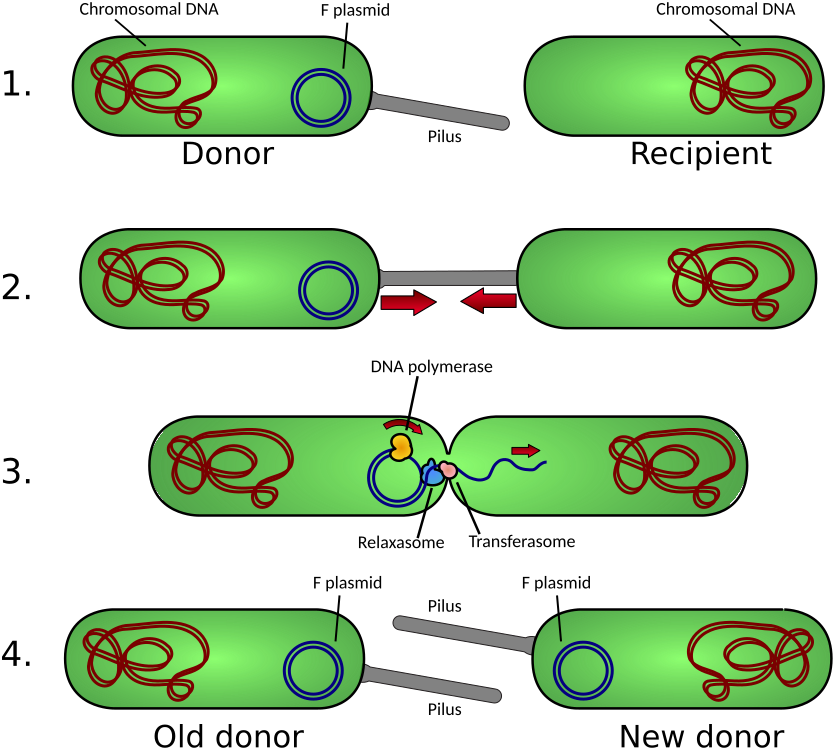
\includegraphics[width=0.7\linewidth]{images/Conjugation.png}
    \caption[Schéma du fonctionnement de la conjugaison]{\textbf{Schéma du fonctionnement de la conjugaison, dans le cas d'un plasmide conjugatif.} (1) Formation d'un pili sexuel par la bactérie donneuse. (2) Contact direct entre les 2 bactéries via le pili. (3) Réplication de l'ADN plasmidique et transfert à la bactérie donneuse. (4) Terminaison de la conjugaison et nouvelle formation d'un pili pour la receveuse devenue donneuse. Image sous licence Creative Commons 3.0 \url{https://commons.wikimedia.org/wiki/File:Conjugation.svg}}
    \label{fig:conjugaison}
\end{figure}

Plasmides et ICEs sont généralement de petite taille, mais ils contiennent des gènes clés d'adaptation à l'environnement. La présence de ces gènes dans les éléments mobiles permet à des colonies de répondre efficacement et rapidement aux nouvelles conditions environnementales, comme la présence de métaux lourds ou d'antibiotiques \cite{botelho_role_2021}. Toutefois, tous les MGEs ne sont pas forcément conjugatifs \cite{valentine_mobilization_1988}, ils vont profiter de la conjugaison codée par un autre élément pour se transférer. Dans ces conditions, la bactérie receveuse ne devient pas conjugative à son tour, même si elle reçoit l'élément mobile. Ces éléments mobilisables sont appelés des IMEs (élément intégratif mobilisable). Il est d'ailleurs à noter que tous les plasmides ne sont pas mobilisables, il y aurait d'ailleurs autant de plasmides conjugatifs que de plasmides non mobilisables \cite{smillie_mobility_2010}.

La conjugaison est un mécanisme majeur de transfert horizontal de matériel génétique, qui a la caractéristique de rapidement répandre les éléments mobiles. Il a toutefois le défaut de limiter le transfert de gènes entre cellules procaryotes et donc de limiter le transfert aux innovations génétiques déjà intégrées par un autre organisme procaryote. De plus, tous les organismes ne sont pas capables de réaliser la conjugaison, ce qui réduit d'autant plus la capacité de transfert au niveau des communautés.

\newpage
\subsubsection{Transformation : recycler l'ADN environnant}

La transformation correspond à l'intégration d'un fragment d'ADN étranger dans le génome de l'organisme. Les bactéries pouvant réaliser la transformation sont dites compétentes. Ce qui  différencie la transformation de la conjugaison, c'est que l'ADN intégré est libre dans l'environnement
\footnote{La découverte de la transformation en 1928 par Fred Griffith \cite{griffith_significance_1928}, précède de nombreuses années celle qui a mis en évidence que l'ADN est le porteur de l'information génétique \cite{avery_studies_1944}. La transformation est donc une preuve anticipée et un socle pour démontrer le rôle de l'ADN.}. De plus, la transformation est la seule forme de HGT, totalement contrôlée par la cellule receveuse \cite{huang_activation_2021}. Assez peu d'espèces sont connues pour être capables de réaliser la transformation de manière naturelle, toutefois un nombre plus important contient  la machinerie nécessaire à sa réalisation \cite{johnston_bacterial_2014}. De plus, au sein d'une espèce, le taux d'individu compétent peut varier, par exemple chez \textit{S. pneumoniae}, 66 \% des individus sont capables de la réaliser \cite{evans_significant_2013}.
Pour terminer, les mécanismes de la transformation, notamment l’incorporation de l’ADN dans la cellule (\autoref{fig:transformation}), sont bien décrits dans la littérature \cite{johnston_bacterial_2014,dubnau_mechanisms_2019}. Toutefois, ils varient d’une espèce procaryote à l’autre, tout comme la proportion d’individus capables de réaliser cette transformation \cite{stewart_biology_1986}. Nous ne reviendrons donc pas sur les mécanismes, mais seulement sur des exemples d'application.

\begin{figure}[htbp]
    \centering
    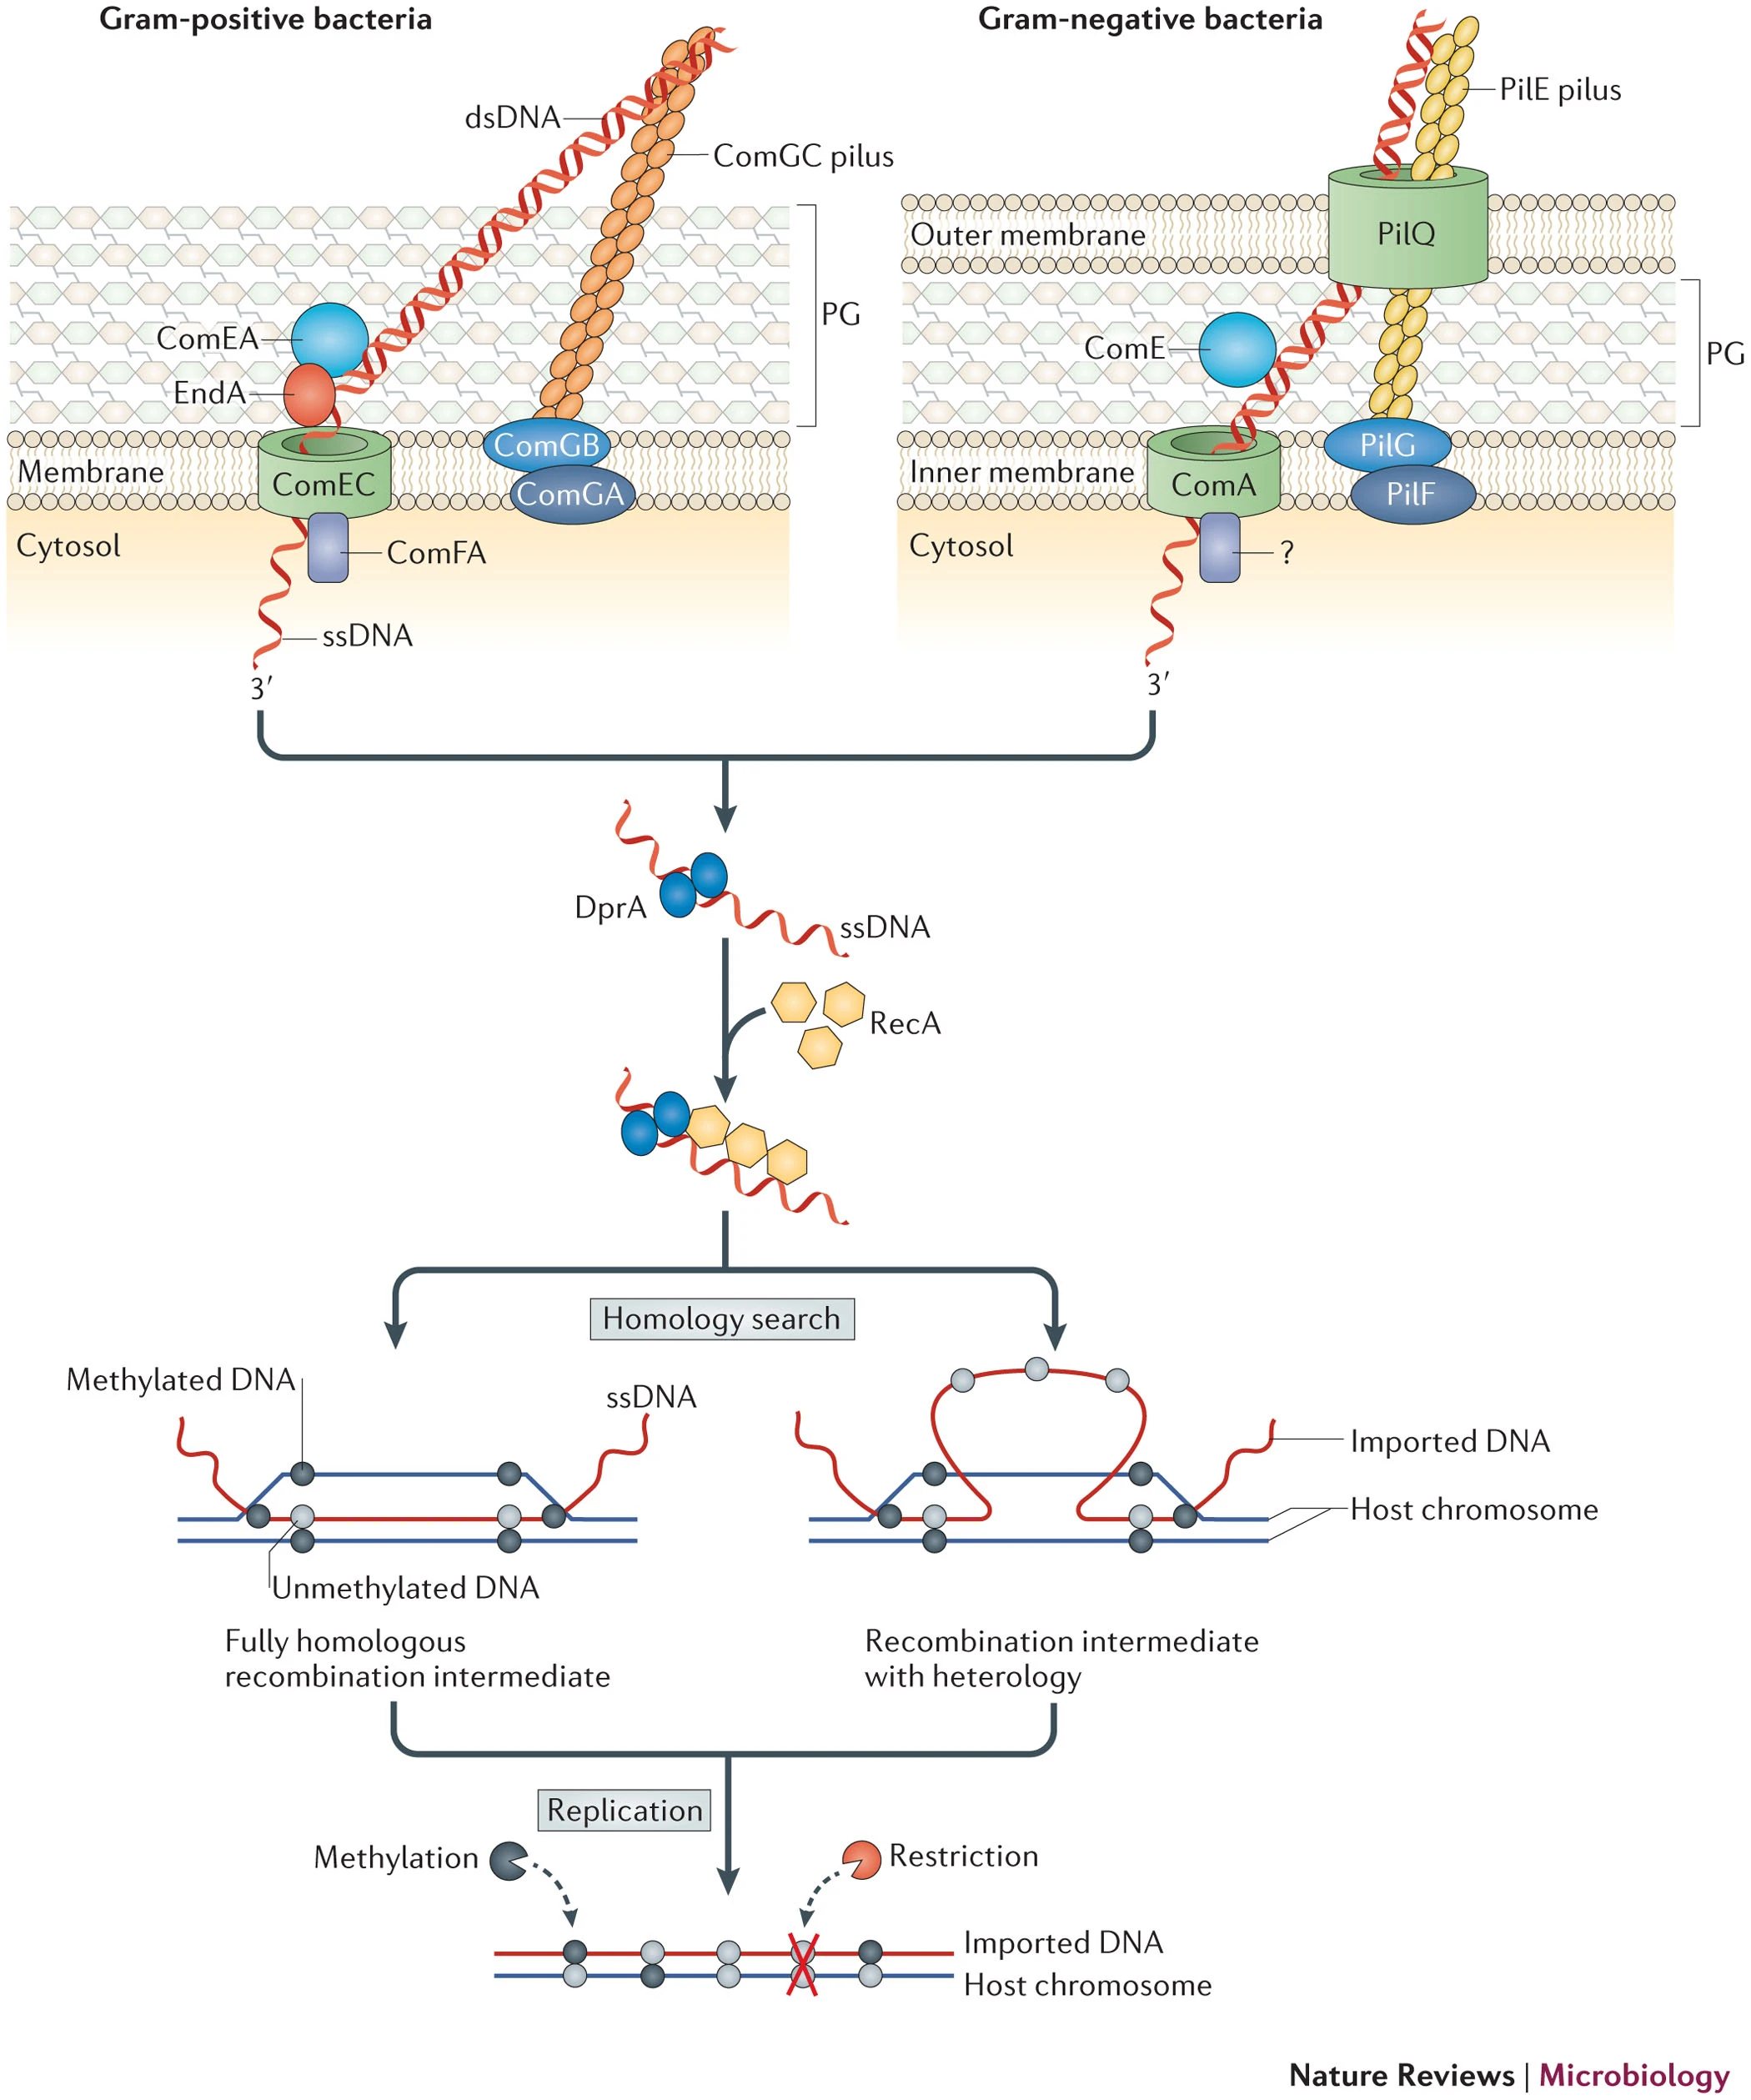
\includegraphics[width=0.625\linewidth]{images/transformation.png}
    \caption[Schéma du mécanisme de transformation]{\textbf{Schéma du mécanisme de transformation.} Extrait de \cite{johnston_bacterial_2014}}
    \label{fig:transformation}
\end{figure}

Les bactéries du genre \textit{Nesseria} et particulièrement \textit{N. gonorrhoeae}\footnote{Ce genre bactérien, vivant dans les muqueuses des mammifères, est non pathogène à l'exception de \textit{N. meningitidis}, impliqué dans la méningite et \textit{N. gonorrhoeae}, responsable de la gonorrhée, une infection sexuellement transmissible.} reconnaissent préférentiellement une séquence d'ADN non palindromique de leur propre ADN \cite{goodman_identification_1988,duffin_dna_2010}. Ce système permet d'intégrer uniquement l'ADN de souches proches, ainsi que des gènes d'adaptation, comme des gènes de résistance aux antibiotiques \cite{centers_for_disease_control_and_prevention_cdc_update_2007}. Ainsi, les gènes d'adaptation d'intérêt sont préférentiellement distribués dans l'espèce.

\textit{Streptococcus pneumoniae}\footnote{Bactérie connue pour son rôle d'agent pathogène dans les pneumonies et responsable de co-infection pendant la grippe espagnole} utilise la transformation comme mécanisme de réparation de l'ADN, car cette espèce ne possède pas de système de réparation SOS \cite{gasc_lack_1980}. Les souches de \textit{S. pneumoniae} s'engagent alors dans une "guerre fratricide" pour récupérer l'ADN des autres souches de leur espèce \cite{claverys_cannibalism_2007}.

Pour terminer, chez \textit{Bacillus subtilis}\footnote{Bactérie du sol, mais qu'on retrouve dans de nombreux habitat dû à ses capacités d'adaptation. Elle est utilisée comme modèle d'étude des bactéries Gram+.}, la transformation entre individus de la même espèce, mais de souche éloignée, est privilégiée \cite{lyons_combinatorial_2016}. Les bactéries vont sécréter dans l'environnement des antibiotiques, auxquels elles sont résistantes, pour tuer les autres individus de l'espèce. L'ADN récupéré est donc différent de celui de la bactérie et donc potentiellement source de nouvelles fonctions.

Ces exemples montrent aussi une opposition dans la philosophie des mécanismes de conjugaison et de transformation. La transformation demande que l'ADN soit libre dans l'environnement et donc que les bactéries environnantes soient détruites, alors que la conjugaison laisse les 2 cellules en vie. 

\subsubsection{Transduction : les virus mis à profit}

La transduction est un mécanisme reposant sur l'intervention d'un virus pour transporter et transférer le matériel génétique d'une cellule procaryote à l'autre (\autoref{fig:transduction}). Les virus de bactéries, surnommés (bacterio)phages, vont infecter la cellule donneuse pour répliquer leur ADN. Lors de la réplication, de l'ADN de la cellule donneuse peut se trouver intégré à celui du phage. Lorsqu'il infectera une cellule receveuse, la portion d'ADN de la donneuse pourra reprendre une forme plasmidique (si c'est un plasmide qui a été transféré) ou être intégrée au génome de la cellule par recombinaison homologue. La transduction est aujourd'hui largement utilisée en génétique et microbiologie pour transférer de l'ADN et modifier les génomes \cite{wang_phage-based_2024}. 

\begin{figure}[htbp]
    \centering
    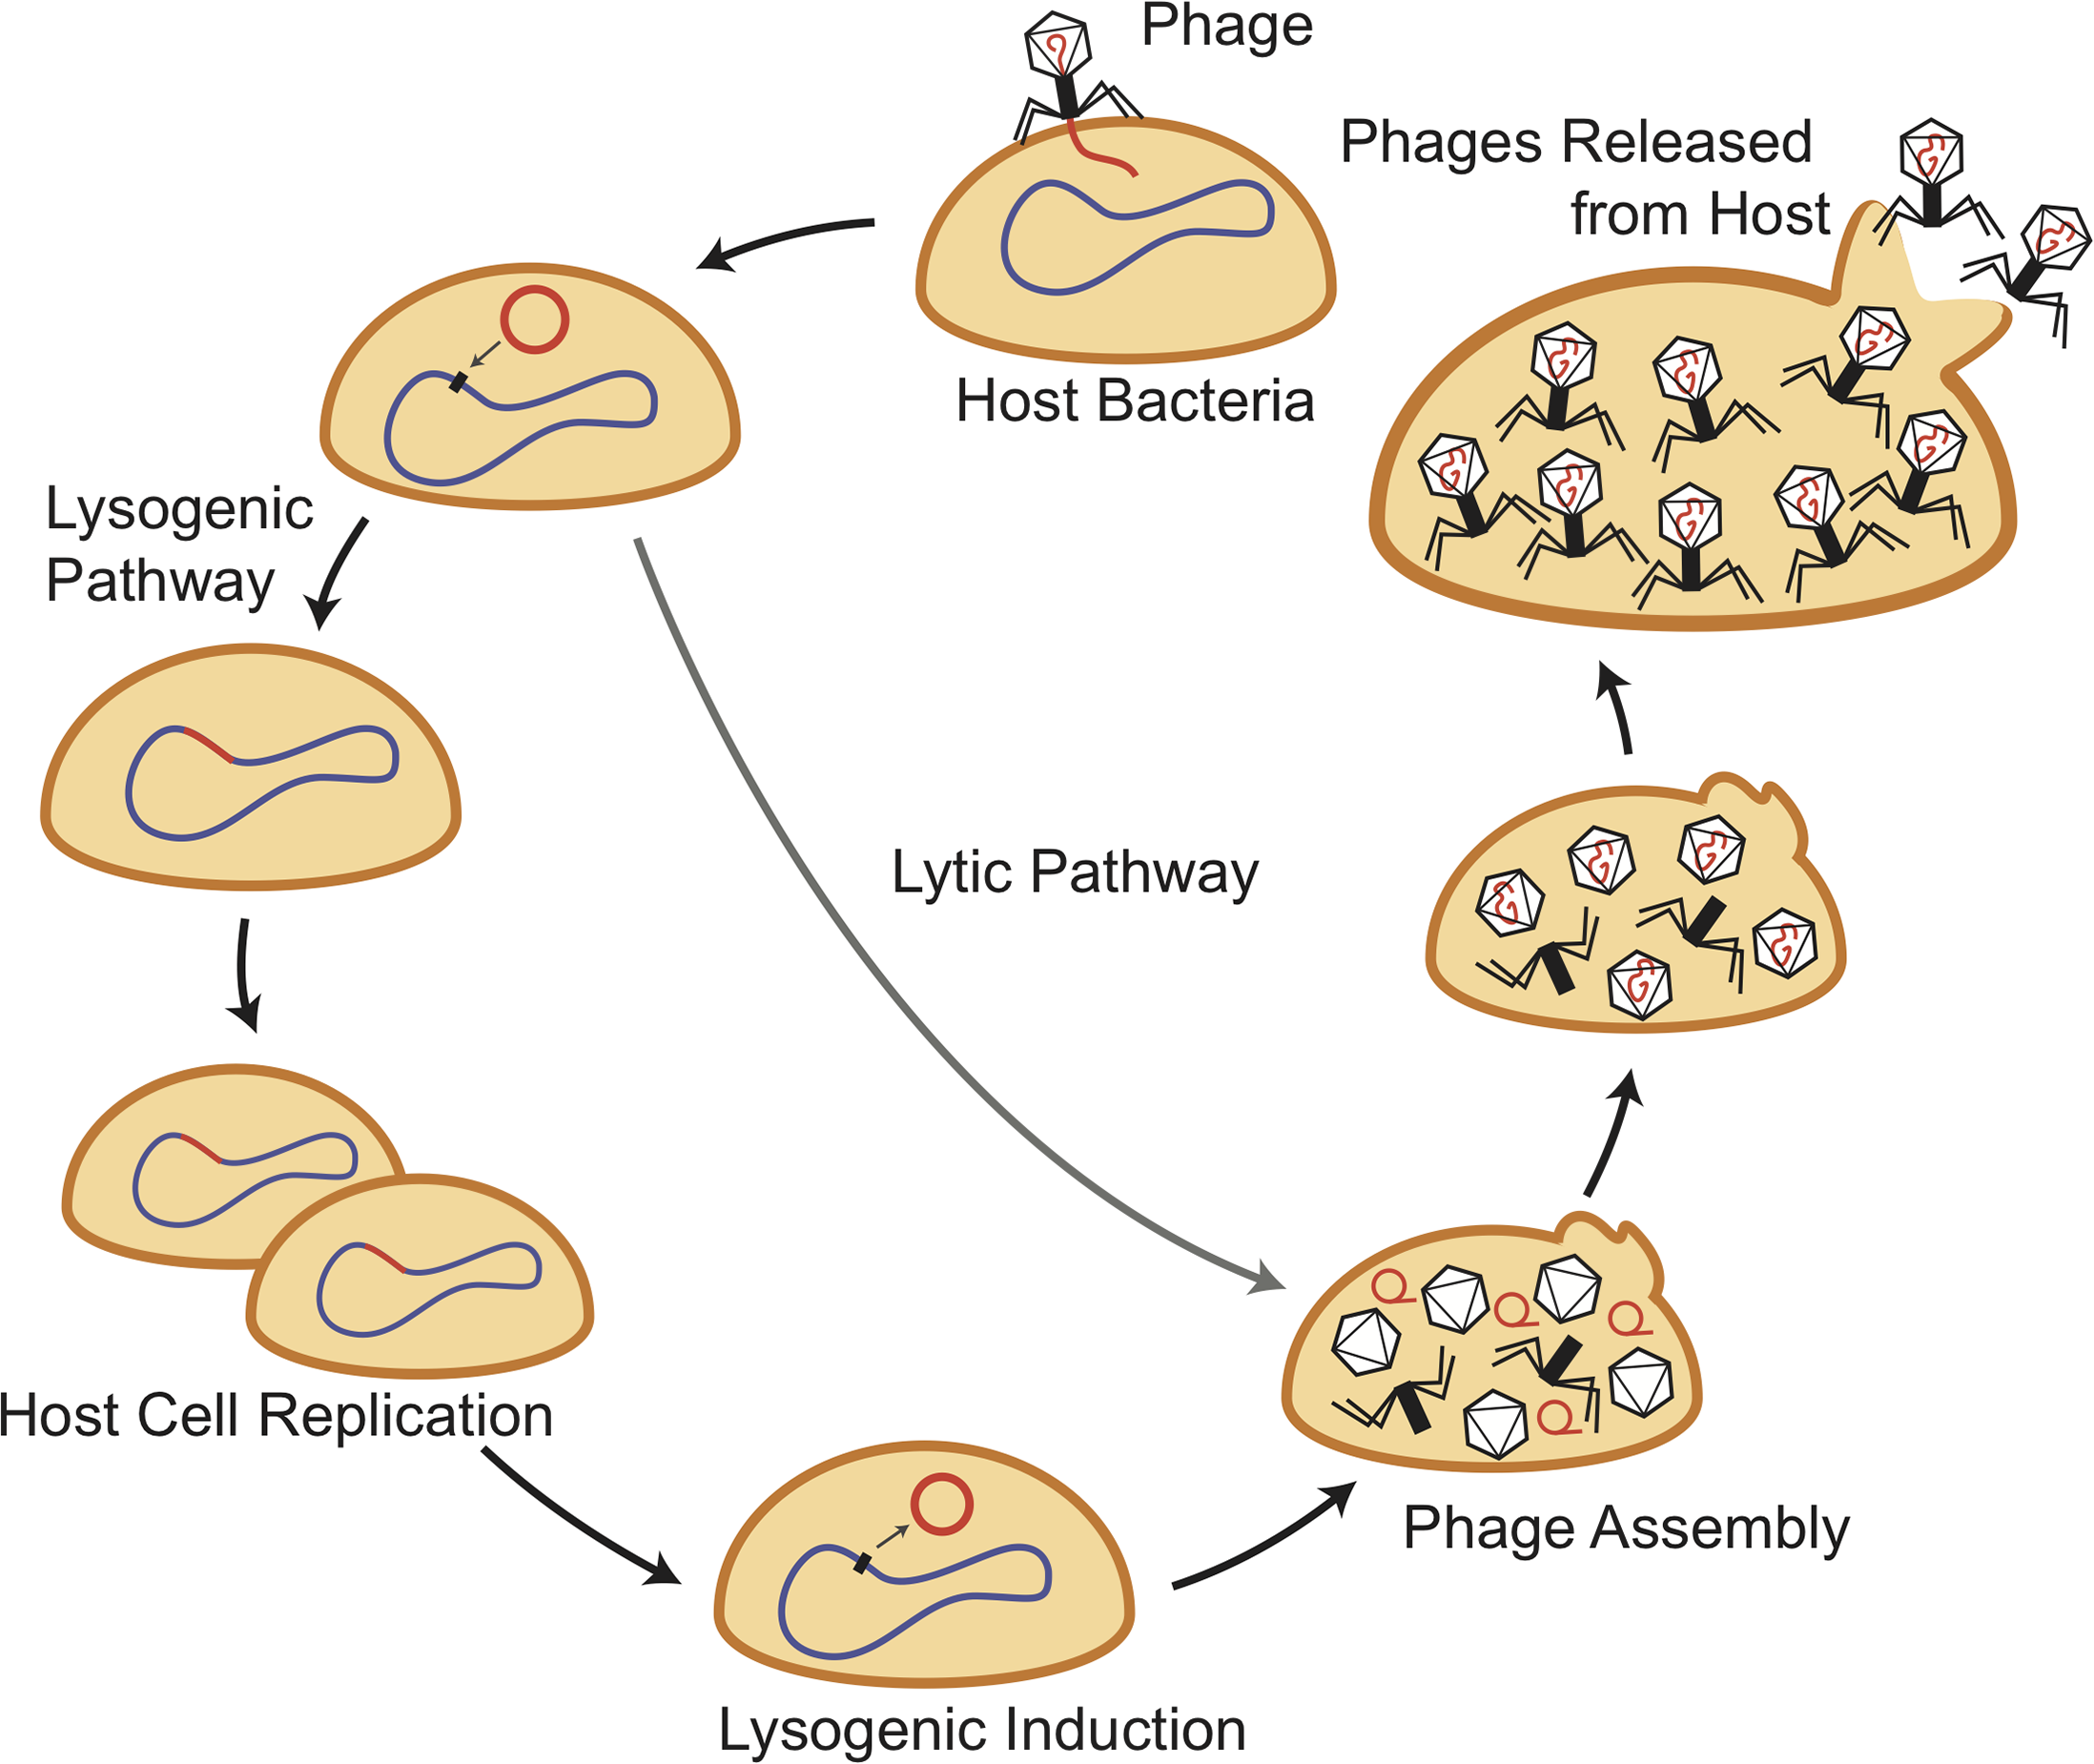
\includegraphics[width=0.65\linewidth]{images/transduction.png}
    \caption[Schéma synthétique de la transduction]{\textbf{Schéma représentant les étapes de transduction.} Extrait de \cite{chiang_genetic_2019}}
    \label{fig:transduction}
\end{figure}

La première forme de transduction identifiée décrivait le transfert de n'importe quel gène de la donneuse à la receveuse par le phage. Cette forme a donc été nommée transduction généralisée \cite{zinder_genetic_1952}. Une seconde forme dite spécifique a été découverte en étudiant le phage $\lambda$ infectant les \textit{E. coli} \cite{morse_transduction_1956}. Le transfert se limite à un ensemble de gènes définis. Enfin, une dernière forme, la transduction latérale, a récemment été découverte \cite{chen_genome_2018}. Là où les formes générale et spécifique peuvent être vues comme une erreur et un événement lié au hasard, la transduction latérale fait partie du cycle de vie du phage, menant à un taux de transfert beaucoup plus important. 

\newpage
\section{Du génome aux processus cellulaires}

\subsection{Gènes : Régulations et fonctions}
\label{sec:fn_reg}

Les réactions qui se produisent dans les cellules procaryotes sont souvent complexes et impliquent une multitude de réactifs et de produits. Toutes ces réactions nécessitent la présence de protéines spécifiques pour être réalisées. Ces protéines sont produites et dégradées par la cellule en fonction des conditions rencontrées. C'est pourquoi l'information est stockée dans une structure durable et transmissible, le gène. Chaque gène sera transcrit en une molécule d'ARN messager (ARNm) par l'ARN polymérase, qui sera traduite en protéine par le ribosome (impliquant l'ARNr et l'ARNt). 


Dans une cellule, les protéines ont un temps de "vie" allant de quelques minutes à quelques heures. Il est donc nécessaire de produire les protéines régulièrement, toutefois cette production a un coût pour la cellule. C'est pourquoi il existe des mécanismes de régulation de l'expression des gènes et donc de la production des protéines. Dans la \autoref{sec:gene}, nous avons vu qu'il existait notamment des petits ARN régulateurs de l'expression. Dans l'ADN non codant, on retrouve également une séquence promotrice (ou promoteur) près d'un gène qui permet la fixation de l'ARN polymérase. La fixation et l'activation de l'ARN polymérase au niveau du promoteur sont régulées par des facteurs de transcription qui se lient spécifiquement à des séquences régulatrices en amont du promoteur, les \textit{enhancer} et \textit{silencer}.


Les protéines peuvent agir en collaboration, soit dans des réactions successives (cas des systèmes biologiques, cf. \autoref{sec:sys_bio}), soit en formant des complexes protéiques interagissant pour métaboliser un produit. Les gènes codant pour des protéines impliquées dans les mêmes processus cellulaires sont situés dans le même contexte génomique (cf. \autoref{sec:gene}). Ils vont alors être régulés par les mêmes éléments de régulation. L'opéron, une structure spécifique des procaryotes découverte par François Jacob et Jacques Monod en 1960\footnote{Découverte qui leur a valu le prix Nobel de médecine en 1965}\cite{jacob_genetic_1961}, permet de produire un seul ARNm pour un ensemble de gènes codant pour des protéines impliquées dans le même processus cellulaire. Dans l'opéron, se trouve une nouvelle séquence de régulation, l'opérateur, où va se lier une molécule régulatrice qui va activer ou inhiber la transcription (\autoref{fig:lac_operon}). L'ensemble de l'opéron permet de synchroniser la régulation et l'expression de gènes qui collaborent dans le même processus cellulaire.


\begin{figure}[htbp]
    \centering
    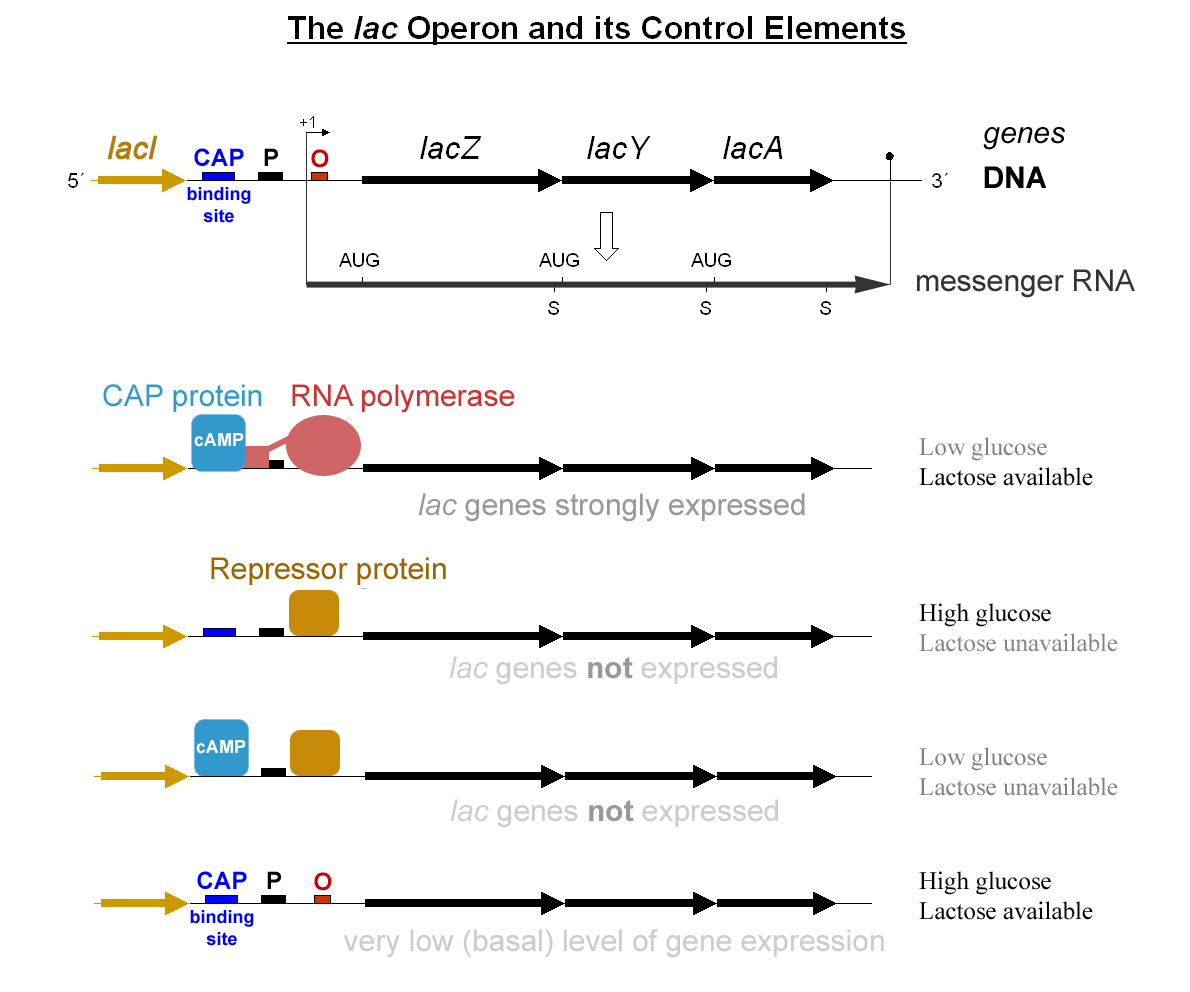
\includegraphics[width=\linewidth]{images/Lac_operon-2010-21-01.png}
    \caption[Exemple de l'opéron lactose]{\textbf{Schéma du fonctionnement de l'opéron lactose.} Sur la partie haute est représenté la structure génétique de l'opéron. Les 4 lignes suivantes représentent chacune une configuration de réponse à des conditions de présence, absence de glucose et de lactose. si le taux de glucose est faible, une protéine activatrice (CAP) va se fixer en amont du promoteur pour aider à la fixation de l'ARN polymérase, et si du lactose est disponible, les gènes seront alors fortement exprimés. Si le lactose n'est pas disponible, une protéine de répression va se fixer à l'opérateur et elle empêchera l'ARN polymérase de se fixer même si le taux de glucose est faible. 
    Auteur : G3pro. Sous licence Creative Commons 2.0. Disponible à l’adresse : \url{https://commons.wikimedia.org/wiki/File:Lac_operon-2010-21-01.png.}
    }
    \label{fig:lac_operon}
\end{figure}

Pour terminer, l'expression des gènes peut aussi être régulée par le niveau de repliement et de condensation de l'ADN. L'ADN est condensé notamment grâce à des protéines spécialisées et à la méthylation de l’ADN. L'ADN replié ne pourra pas être accessible pour la transcription des gènes et donc ils seront inactifs. Les mécanismes liés à la méthylation de l'ADN sont l'affaire de l’épigénétique. Des études récentes ont mis en lumière le rôle de la méthylation dans la régulation de la virulence bactérienne et dans la capacité des procaryotes à coloniser leurs hôtes \cite{oliveira_bacterial_2021}, soulignant ainsi l'importance de ces mécanismes dans la survie et l’adaptation des bactéries.

\newpage
\subsection{Îlots génomiques et points chauds d'insertion}
\label{sec:ilot}
Les îlots génomiques (GI, pour \textit{Genomic Island en anglais}) sont des régions spécifiques du génome qui jouent un rôle clé dans l'évolution, l'adaptation et l'acquisition de fonctions spécifiques. Les GIs sont retrouvés chez quasiment tous les organismes procaryotes. Ils sont généralement acquis par transfert horizontal (cf. \autoref{sec:evo_hz}) et transportent des gènes accessoires. Ils vont conférer à l'organisme de nouvelles fonctions qui impacteront de façon positive sa \textit{fitness}. Le premier îlot génomique décrit était lié à la capacité de la bactérie \textit{E. coli} de provoquer des maladies et a donc été nommé îlot de pathogénicité \cite{hacker_deletions_1990}.  Depuis, d'autres classes d'îlots ont été découvertes : métabolique, résistance, symbiotique\dots (\autoref{fig:GI}).

Les îlots génomiques sont des régions assez larges, entre 5 et 200 kb (mais certaines sont beaucoup plus grandes) et présentent des caractéristiques spécifiques. (\textit{i}) Les GIs ont un taux de GC qui diffère par rapport au reste du génome, résultant en un biais d'usage des codons\footnote{Un biais d'usage des codons, désigne la fréquence d’utilisation préférentielle de certains codons parmi les codons synonymes pour coder un même acide aminé.} (\autoref{fig:GI}). (\textit{ii}) dans les régions flanquantes des GIs, on retrouve des gènes de mobilité : transposases et intégrases, mais aussi d'IS qui peuvent se dégrader rapidement après l'intégration de l'îlot. (\textit{iii}) Dans les gènes flanquants, on retrouve des gènes codant l'ARNt dont l'origine serait à relier à la prévalence des gènes de phages et des ICEs qui utilisent les ARNt comme site d'intégration dans les génomes \cite{dobrindt_genomic_2004}. (\textit{iv}) Les protéines contenues dans les GIs ont souvent des fonctions inconnues. (\textit{v}) Dans la partie flanquante, on trouve des séquences répétées directes\footnote{Séquences identiques présentes en plusieurs copies dans la même molécule d'ADN et ayant la même orientation.}.

\begin{figure}[htbp]
    \centering
    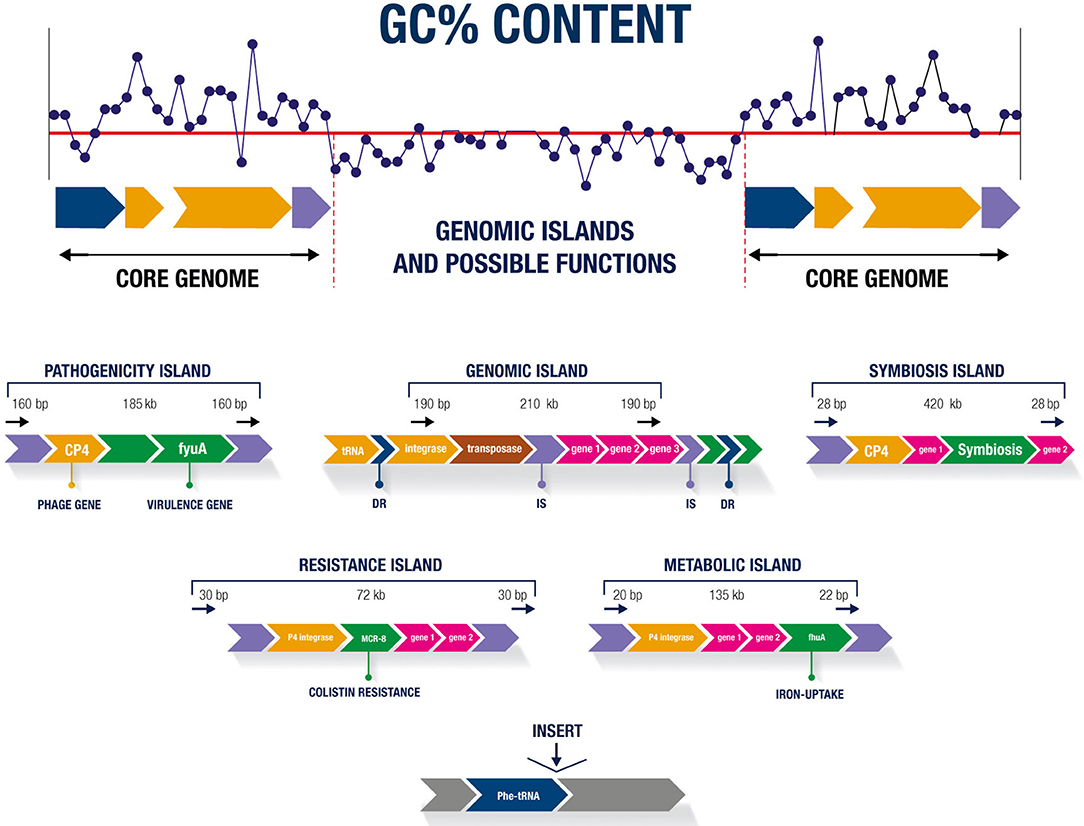
\includegraphics[width=0.8\linewidth]{images/ilot_genomique.jpg}
    \caption[Îlots génomiques et leur caractéristique]{\textbf{Îlots génomiques et leur caractéristique.} Extrait de  \cite{da_silva_filho_comparative_2018}}
    \label{fig:GI}
\end{figure}

\newpage
Ces GIs sont complexes à étudier, car ils concentrent les variations, même entre génomes proches. L'histoire évolutive est souvent difficile à reconstituer, tant des éléments ont été intégrés et éliminés au cours du temps (\autoref{fig:cycle_IG}). En plus de s'échanger avec d'autres organismes \cite{buchrieser_high-pathogenicity_1998}, les GIs peuvent se déplacer au sein du génome \cite{karaolis_bacteriophage_1999}.

\begin{figure}[htbp]
    \centering
    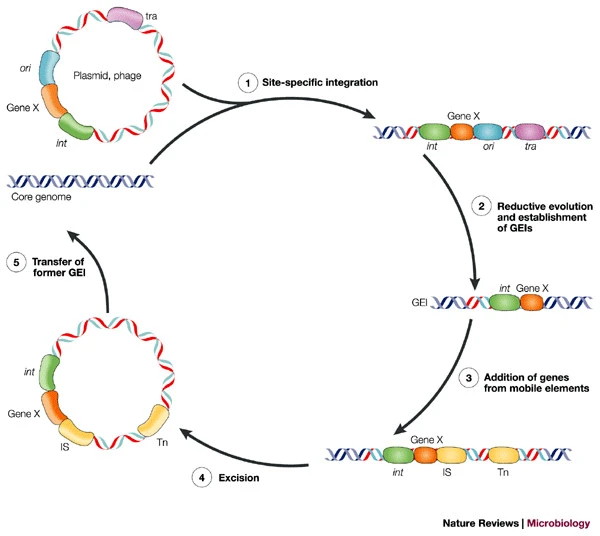
\includegraphics[width=0.65\linewidth]{images/cycle_GI.png}
    \caption[Cycle de vie d'un îlot génomique]{Cycle de vie d'un îlot génomique. Extrait de \cite{dobrindt_genomic_2004}}
    \label{fig:cycle_IG}
\end{figure}

Les GIs ne s'insèrent pas n'importe où dans les génomes. On les retrouve fréquemment dans des zones où de nombreux éléments se sont insérés au cours de l'évolution d'un taxon. Ces régions sont appelées : point chaud d'insertion (\textit{hotspot} en anglais).
À l'intérieur des \textit{hotspots}, on retrouve une grande variabilité du contenu génique entre les génomes. Les \textit{hotspots} sont également caractérisés par des bordures composées de gènes communs à l'ensemble des génomes. 

Ils présentent également une recombinaison homologue accrue dans les gènes flanquant les \textit{hotspots}, avec 50 \% d’événements de recombinaison et 30 \% d’incongruence phylogénétique\footnote{L'incongruence phylogénétique désigne une discordance entre l’arbre phylogénétique d’un gène spécifique et l’arbre phylogénétique global construit à partir d'un grand nombre de gènes conservés.} par rapport à l'arbre des espèces. Ces \textit{hotspots} contiennent 50 \% des gènes acquis par HGT \cite{oliveira_chromosomal_2017}. Ils sont enrichis en gènes liés à la motilité, à la défense, à la transcription, à la réplication et à la réparation de l’ADN \cite{flores_ramos_genomic_2021}.

Le contenu génique du \textit{hotspot} provient d'une accumulation progressive de gènes, comme le suggère le faible pourcentage (8 \%) de \textit{hotspots} composés uniquement de gènes spécifiques à une souche \cite{oliveira_chromosomal_2017}. Cette accumulation peut se faire par bloc de gènes. Ces blocs, conservés dans le \textit{hotspot}, sont appelés modules \cite{lescat_module_2009}. Cette modularité pourrait expliquer l'organisation complexe des îlots génomiques \cite{touchon_organised_2009}.
Les \textit{hotspots}, sont donc communs à un groupe d'organismes, et définis au niveau d'un taxon. Il est donc nécessaire de mener des études de comparaison des génomes pour les identifier.
\chapter{Génomique comparées des procaryotes}
\section{Analyse comparative des génomes : méthodes et applications}
\label{sec:comp_gen}
\subsection{Comparaison des séquences}
\subsection{Statistique et séquence}
\subsection{Utilisation des graphes}
\subsection{Application de la génomique comparée pour l'étude des procaryotes}
\subsection{Intelligence artificielle : machine learning et deep learning}
\section{Système biologique}
\subsection{Définition et intérêt}
\subsection{Méthode de détections}
\subsection{Systèmes de défense aux phages}
\chapter{Pangénomique: état des lieux, enjeux et ambitions}

 La pangénomique est un domaine d'étude en plein essor, qui a permis d'explorer et d'analyser les génomes procaryotes sous un nouveau point de vue. Mon travail de thèse s'est concentré sur l'analyse et la comparaison de pangénomes. Dans cette partie, je reviendrai d'abord sur l'origine, les concepts et les défis que pose la pangénomique.  Je présenterai ensuite les différentes modélisations permettant de représenter les génomes en pangénomique, pour poursuivre sur les méthodes de construction de pangénome. Pour terminer, je développerai les méthodes d'analyse existantes en pangénomique. Cette partie sera aussi l'occasion de faire l'état de l'art des outils en pangénomique et de présenter l'outil PPanGGOLiN sur lequel j'ai pu travailler et que j'ai utilisé dans mes développements de thèse.

\section{Origine, concept et défis}

Bien que le terme "pangénome" soit utilisé dans des articles avant 2005, en microbiologie, on s'accorde sur une origine du concept de pangénome proposé dans 2 articles fondateur \cite{medini_microbial_2005,tettelin_genome_2005}. L'idée est alors de ne pas représenter les génomes individuellement, mais d'utiliser une structure mathématique pour les représenter tous en même temps. Le pangénome représente donc l'union de toutes les séquences présente dans un ensemble de génome. Entre 2006 et 2024, ce n'est pas moins de 3 500 articles qui référencent le terme\footnote{Ce chiffre doit être revue à la baisse dû à l'utilisation erronée du terme dans certaines études et une utilisation parfois abusive pour profiter de l'intérêt croissant pour ces analyses}, dont près de 800 concernant les procaryotes (\autoref{fig:panCite}). En bioinformatique, la structure, les algorithmes, les méthodes d'analyses des pangénomes, ont constitué un nouveau champ de recherche, la pangénomique.

\begin{figure}[htbp]
    \centering
    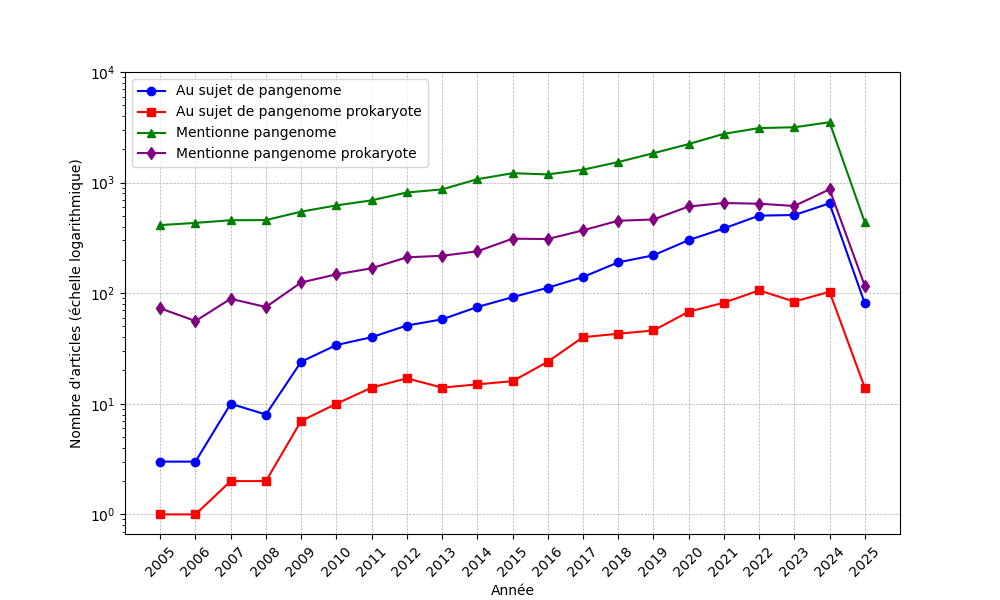
\includegraphics[width=\linewidth]{images/pangenomeCitation.png}
    \caption[Bibliométrie pangénome]{Nombre d'articles, référencé dans PubMed, par année, à propos de pangénome de 2004 au 10 février 2025. La courbe bleue représente le nombre d'articles contenant le terme pangénome dans le titre ou l'abstract : Query=("pan-genome"[Title/Abstract] OR "pangenome"[Title/Abstract] OR "pan-genome"[Title/Abstract]) AND (2004:2025[pdat]). La courbe rouge limite aux publications concernant les procaryotes : Query=("procaryote"[Title/Abstract] OR "bacteria"[Title/Abstract] OR "archeae"[Title/Abstract]) AND ("pan-genome"[Title/Abstract] OR "pangenome"[Title/Abstract] OR "pan-genome"[Title/Abstract]) AND (2004:2025[pdat]). La courbe verte représente tous les articles ou le terme pangénome est trouvé : Query=((pangenome) OR (pan genome)) OR (pan-genome) AND (2004:2025[pdat]). La courbe violette filtre les publications concernant les procaryotes : Query=(((procaryote) OR (bacteria)) OR (archeae)) AND (((pan-genome) OR (pangenome)) OR (pan genome)) AND (2004:2025[pdat]).}
    \label{fig:panCite}
\end{figure}

Le pangénome est une structure de données complexes qui peut contenir un ensemble d'informations. Notamment, à partir du pangénome, Tettelin \textit{et al.} propose de séparer les gènes en 2 catégories, les gènes "\textit{core}" commun à tous les génomes, des gènes "\textit{dispensable}" trouver dans un sous-ensemble de génomes. En généralisant, le pangénome permet de distinguer l'ensemble des séquences communes à tous les organismes, des variations présente chez certains groupes d'individus, voire spécifique à un organisme. De ce postulat a émergé l'idée de remplacer les génomes de références dans les bases de données par des pangénomes de références. Toutefois, ce changement de paradigme n'a pas encore été opéré, car il pose plusieurs questions. La première est la question de la représentation des pangénomes, nous aborderons les modèles et représentations des pangénomes, qui doit être visualisable par l'\oe il humain, tout en intégrant l'ensemble de l'information du pangénome. La seconde question est celle du stockage, les génomes sont généralement stockés sous forme de texte et relié à leurs informations dans des bases de données. Le pangénome est une structure plus complexe, qui n'est pas possible de stocker sous forme de texte. De plus, les bases de données contenant les pangénomes doivent pouvoir être interrogé de façon efficace. Étant donné l'augmentation du volume de données génomique dans les bases, il est également nécessaire que la base de données puissent être mise à jour régulièrement. La dernière question, essentiel, est : quelle méthode utiliser pour construire le pangénome ? Il faut tout d'abord définir les éléments qui constituent le pangénome, \textit{i.e.}, les gènes ou des k-mers pour les variants, ou encore des séquences d'ADN plus longues. Il faut ensuite connecter ces éléments, selon des critères pertinents. Enfin, il faut pouvoir donner un sens au pangénome et donc il faut pouvoir y appliquer des algorithmes pour l'analyser. Toutes ces questions n'ont pas encore trouvé de réponse consensus dans la communauté et aucune méthode n'a encore réussi à s'imposer comme solutions optimales. Trouvé une méthode globale est aussi un défi, car la pangénomique est appliqué dans de nombreux domaines de recherches, pour répondre à une grande diversité de question.

La pangénomique est largement utilisée dans de nombreux domaines. Le "Computational Pan-Genomics Consortium" met en avant son rôle dans le développement de solutions applicatives répondant à des problématiques communes à plusieurs disciplines \cite{the_computational_pan-genomics_consortium_computational_2018}. Elle bénéficie ainsi des avancées en phylogénie, métagénomique et intelligence artificielle.

En phylogénie, les méthodes de comparaison génomique à grande échelle et les techniques de construction d'arbres phylogénétiques ont été intégrées aux approches pangénomiques. En retour, la pangénomique permet une meilleure prise en compte des variations génétiques à l'échelle de l'ensemble des génomes, plutôt que de se limiter à un génome de référence, offrant ainsi une vision plus fine de la dynamique évolutive.

En métagénomique, les outils d’assemblage ont été adaptés pour affiner la reconstruction des pangénomes. Les algorithmes de \textit{binning}\footnote{Procédure de regroupement des contigs assemblé et d'assignation à un génome d'origine.} et de profilage génétique facilitent l’identification de clusters de gènes conservés et variables. En retour, la pangénomique enrichit l’analyse de la diversité génétique au sein des communautés microbiennes, dépassant ainsi la seule représentation de la diversité des génomes au sein d’un taxon.

L’intelligence artificielle joue également un rôle clé en améliorant l’annotation et la prédiction fonctionnelle des gènes. L’apprentissage automatique est appliqué à la pangénomique pour détecter des motifs génétiques pertinents, prédire des phénotypes et identifier des associations entre mutations et traits phénotypiques.

Ces méthodes, souvent développées pour d’autres disciplines, ont donc favorisé l’essor de la pangénomique en optimisant l’analyse des données, la reconstruction des génomes et l’interprétation des résultats.

La pangénomique se présente donc comme une solution à l'analyse de grand volume de données, à l'heure où le nombre de génomes disponible dans les banques augmentent de façon exponentielle, mais apporte aussi son lot de défis.

\subsection{Modélisation de la croissance des pangénomes}
\label{sec:croissance_pan}

Dans l'article original de Tettelin \textit{et al.}, les auteurs s'intéresse à la distribution \textit{core/dispensable} en fonction du nombre de génomes de \textit{Streptococcus agalactiae}\footnote{Bactérie du microbiote intestinale humain et animal, qui est également associé à des infections graves.} que contient le pangénome. Ils observent que lorsque le nombre de génomes augmente, la part de \textit{core genome} décroît de façon exponentielle. Ce résultat les amène à modéliser la croissance du \textit{core genomes} selon une équation exponentielle décroissante. Le modèle permet alors d'estimer la taille du \textit{core genome} pour un nombre de génomes en théorie infinie. Il est alors possible d'estimer la taille du \textit{core genome} d'une espèce à partir d'un échantillon de génome. 

À partir de ce modèle, il est également possible d'estimer la taille du pangénome, \textit{i.e.}, le nombre de gènes unique que contient le pangénome. Ils définissent alors 2 types de pangénomes en fonction de l'estimation de la taille : les pangénomes ouvert et les pangénomes fermés. Les pangénomes sont considérés comme ouverts lorsque le nombre de gènes ajouté au pangénome lors de l'ajout d'un nouveau génome, ne diminue pas avec l'ajout de nouveaux génomes. Le nombre de gènes est donc théoriquement infini pour un pangénome ouvert avec une infinité de génomes. Les pangénomes fermé quant à eux voit le nombre de nouveaux gènes progressivement diminué lors de l'ajout de nouveaux génomes. La courbe de prédiction permet d'identifier un plateau théorique du nombre maximal de familles que contiendra le pangénome avec un nombre de génomes infinis. Biologiquement, le pangénome ouvert est attendu pour les espèces sympatriques\footnote{Espèces vivant dans le même environnement que d'autres espèces.} et qui présentent un fort taux de transfert horizontaux, tandis que les espèces vivant dans des niches écologiques ou qui ont une faible capacité d'acquisition de gènes extérieurs vont avoir un pangénome fermé.

\begin{figure}[htbp]
    \centering
    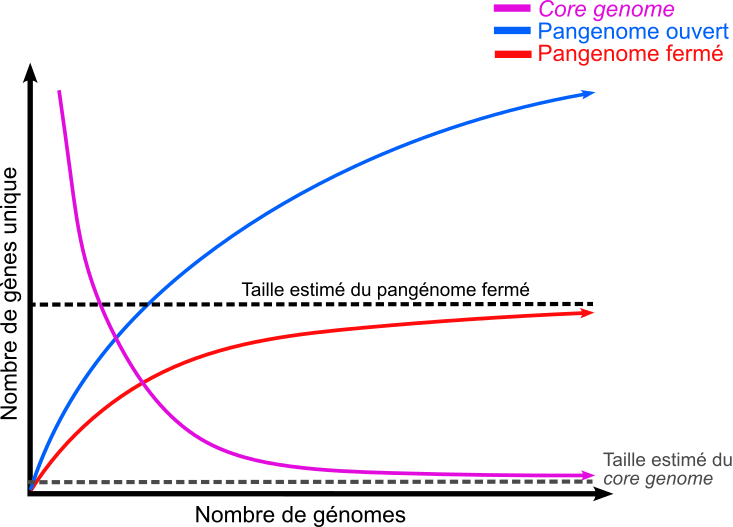
\includegraphics[width=0.7\linewidth]{images/panOpenClose.png}
    \caption[Schéma de croissance du pangénome]{Schéma de croissance du pangénome.}
    \label{fig:panOpenClose}
\end{figure}

Le modèle proposé par Tettelin \textit{et al.}, repose sur l'hypothèse que pour un nombre suffisant de génomes, le nombre de nouveaux gènes apporté par un génome devient constant à partir d'un certain nombre de génomes. Cette hypothèse implique alors que la taille du pangénome est infinie. Cette hypothèse sera questionnée par Hogg \textit{et al.} dans leur étude du pangénome de \textit{Haemophilus influenzae} \cite{hogg_characterization_2007}. Ils vont alors proposer une modélisation basée sur l'hypothèse que le pangénome est fini. Dans leur modèle, chaque gène est associé à une variable aléatoire de Bernoulli, dont la probabilité correspond à la fréquence du gène dans les génomes. Un génome est ainsi généré en observant ces variables : un gène est présent si l’essai est un succès, sinon il est absent. Bien que certains gènes ne soient pas indépendants en raison de structures comme les îlots génomiques, cette hypothèse est conservée pour simplifier le modèle. Les fréquences réelles des gènes étant inconnues, elles sont modélisées de manière probabiliste en répartissant les gènes en $K$ classes distinctes, chacune ayant une fréquence de présence spécifique. À partir de ce modèle, sur le pangénome de \textit{H. influenzae} avec $K=7$, la taille du pangénome est estimé à 5 000 gènes (contre 2 800 gènes dans les 13 génomes de bases). Ce modèle sera ensuite amélioré par Snipen \textit{et al.} \cite{snipen_microbial_2009}, qui proposeront une détermination automatique du nombre de classes $K$ et de la fréquence théorique des gènes pour chaque classe. Les modèles binomiaux propose une perspective dans laquelle la diversité en gènes est finie et qu'il existe un nombre de génomes suffisamment grand pour que tout le répertoire génique soit connu. Cette vision semble de prime abord logique, car le nombre de combinaisons possible de nucléotide ou d'acide aminé est fini. Pourtant, on peut y opposer que ce nombre, sans le calculer, semble démesuré et qu'il peut être considéré comme infini. De plus, les génomes évoluent continuellement et que de nouveaux gènes apparaissent sans cesse. L'utilisation des modèles binomiaux semble alors plus approprié à des espèces de niche, isolé et présentant un faible taux de transfert horizontaux.

En 2008, Tettelin \textit{et al.} vont proposer une nouvelle modélisation basée sur la loi de Heaps\footnote{Définit de manière empirique en linguistique, cette loi permet de décrire le nombre de mots d'une langue à partir d'un ensemble de documents.} \cite{tettelin_comparative_2008}. On estime le nombre $n$ de gènes distincts, en fonction du nombre $N$ de génomes étudiés, selon la relation :
\begin{equation}
    n=kN^\gamma, 0<\gamma<1,k\geq1
\end{equation}

Le paramètre $k$ est une constante de proportionnalité tandis que $\gamma$ reflète la tendance de la fonction. Ainsi, plus $\gamma$ est proche de 0 plus la croissance en gène distinct est lente, et plus $\gamma$ est proche de 1 plus la croissance est rapide (\autoref{fig:HeaplawGamma}).

\begin{figure}[htbp]
    \centering
    \subfloat[]{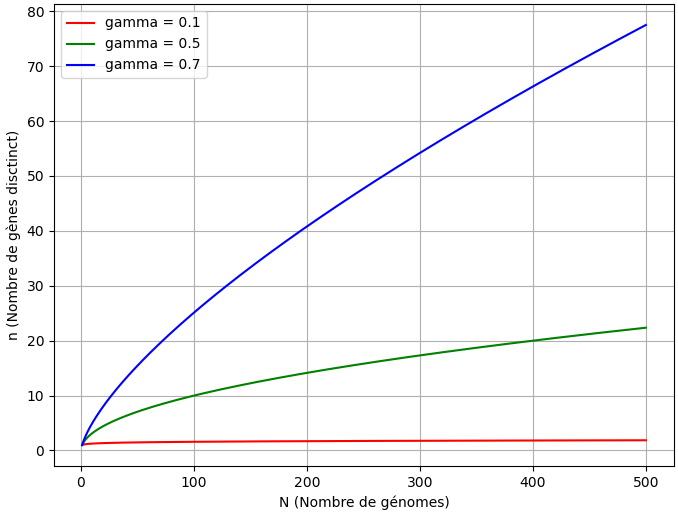
\includegraphics[width=0.48\linewidth]{images/HeapsLawgamma.png}
    \label{fig:HeaplawGamma}}
    \hfill
    \subfloat[]{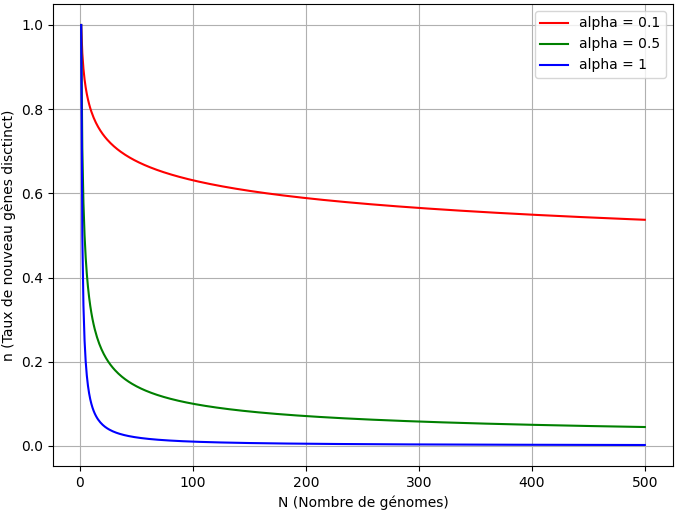
\includegraphics[width=0.48\linewidth]{images/HeapsLawAlpha.png}
    \label{fig:HeaplawAlpha}}
    \caption{Caption}
    \label{fig:Heaplaw}
\end{figure}

Selon la loi de Heap, le nombre de nouveau gènes découvert diminue à mesure que l'on ajoute des génomes. On peut formuler ceci selon l'équation : 

\begin{equation}
    p(n)=kN^{(\gamma-1)}=kN^{-\alpha}, \alpha=1-\gamma
\end{equation}

Ainsi, sur la \autoref{fig:HeaplawAlpha}, lorsque $0<\alpha<1$, le taux de nouveaux gènes décroit en ajoutant des génomes, sans jamais être nulle. Dans ce cas, le nombre de gènes distinct est croissant. Ce qui implique que si $0<\alpha<1$, le pangénome est ouvert. À partir d'un ensemble de génome, il est possible d'estimer k et $\alpha$ (ou $\gamma$) et donc de caractériser si le pangénome est ouvert. Si $\alpha\geq1$, alors le taux de nouveaux gènes atteint 0, ce qui correspond à un pangénome fermé. 

\subsection{Les différents types de pangénomes}

Les pangénomes peuvent être divisés en 2 catégories en fonction de l'unité choisit pour les construire. Le premier type, celui présenté par Tettelin \textit{et al.} \cite{tettelin_genome_2005}, utilise les gènes comme unité de base du pangénome (\autoref{fig:panType}.B). En regroupant les gènes par homologie (appelé famille de gènes, cf. \autoref{sec:fam}), il est possible d'obtenir la présence/absence de gènes similaire dans les génomes. Ces pangénomes ont l'avantage d'être moins couteux en ressources de calcul pour être construit. De plus, ils sont faciles à interpréter, car les gènes sont des unités déjà bien définies et parfois, ils sont même annotés fonctionnellement. Néanmoins, en utilisant les gènes, la méthode d'annotation à un impact important sur le pangénome et il est sensible aux erreurs d'annotation. De plus, les régions non codantes ne sont pas prises en compte dans cette approche. Enfin, les SNPs peuvent passer inaperçu après le regroupement, ainsi que les variants structuraux (SV).

L'autre type de pangénome est basé sur les séquences brutes des génomes. Cette approche plus récente, qui peut être associé à l'outil GenomeMapper \cite{schneeberger_simultaneous_2009}, permet d'identifier les parties similaires des parties variables à partir d'un alignement complet des séquences découpé en k-mers (\autoref{fig:panType}.C,D). Cette approche a l'intérêt de prendre en compte toute la diversité des génomes (codant, non codant, SNPs et SV). Toutefois, la construction de ces pangénomes est plus coûteuse en ressources. De plus, l'interprétation est plus complexe, car le pangénome n'est pas annoté au départ. Pour terminer, certaines méthodes de construction, utilise un génome de référence comme séquence de base (\autoref{fig:panType}.C), ce qui peut aussi introduire un biais.

\begin{figure}[htbp]
    \centering
    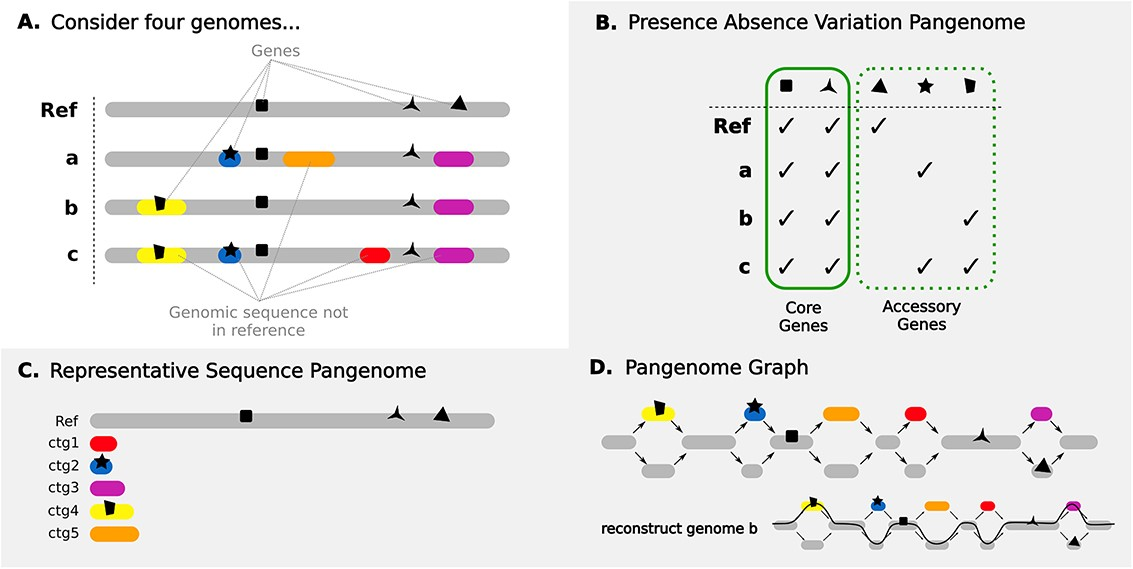
\includegraphics[width=0.8\linewidth]{images/pangenomeTypes.jpeg}
    \caption[Différents types de pangénomes]{Différents types de pangénomes. Extrait de \cite{matthews_gentle_2024}}
    \label{fig:panType}
\end{figure}

\newpage
\section{Pangénome de séquences}

\subsection{Pangénome basé sur une séquence représentative}

Un pangénome basé sur les séquences correspond à un ensemble de génomes dont l'alignement minimise le nombre de régions homologues tout en rendant compte de toute la diversité. L'objectif derrière ces pangénomes est d'obtenir une séquence pangénomique de référence. De façon contre-intuitive (par rapport à la définition "sans-référence" des pangénomes), pour construire ces pangénomes, on utilise une séquence représentative comme base. Toutes les séquences seront alignées à partir de cette base, et les segments non redondants détectés dans au moins un génome seront intégrés à la référence non redondante (NRR, Non-Redundant Reference en anglais). L'ensemble, séquence représentante et NRRs, forme alors la séquence pangénomique de référence.

\subsubsection{Méthode de construction}

Pour construire ces pangénomes, il faut d'abord identifier une séquence représentative. Les autres séquences, en général des séquences non assemblées (lectures ou \textit{reads} en anglais), sont alignées contre la représentante et les séquences non alignables sont considérées comme des NRRs potentiels. Les NRRs de taille inférieure à 500 pb sont exclues, ainsi que celles dont la similarité avec la représentante est supérieure à un seuil (90 \% en général). Les NRRs restantes sont comparées à des bases de données pour retirer tous les contaminants potentiels. De ce schéma général, on peut identifier 4 méthodes différentes pour l'identification des NRRs potentiels :
\begin{itemize}
    \item \textbf{Assemblage de type métagénomique} : les lectures non alignées sur la référence sont regroupées et assemblées \textit{de novo}. Les contigs obtenus sont ajoutés à la séquence représentante. Cette méthode est efficace même avec une faible couverture des lectures.
    \item \textbf{Assemblage itératif} : Dans un premier temps, les lectures non alignées du premier échantillon sont assemblées et ajoutées au génome de référence. Ce génome mis à jour sert ensuite de base pour l’assemblage des échantillons suivants. Ce processus est répété pour tous les échantillons.
\end{itemize}
\newpage
\begin{itemize}
    \item \textbf{Assemblage indépendant des \textit{reads} non alignés} : Toutes les lectures non alignées sont séparées par échantillon\footnote{Ensemble de lectures obtenues simultanément} et assemblées \textit{de novo} indépendamment. Les contigs obtenus sont regroupés selon leur similarité. Dans chaque groupe, un contig référent est identifié et est intégré à la séquence référente. Cette méthode nécessite une couverture d’au moins 10×, pour obtenir des contigs de taille suffisante.
    \item \textbf{Assemblage génomique indépendant} : chaque échantillon est assemblé indépendamment, et les contigs obtenus sont alignés à la référence. Les contigs non alignés sont regroupés par similarité et un contig référent est ajouté à la séquence référente.
\end{itemize}

Le choix de la méthode dépend du type et de la quantité des données disponibles. Avec une faible couverture (<10×) et un grand nombre d’échantillons, l’approche métagénomique est recommandée, bien qu’elle puisse produire des contigs chimériques. Avec une couverture plus élevée (>10×), l’assemblage indépendant ou l’approche itérative sont préférables. Cette dernière est plus lente, mais facilite l’ajout de nouveaux échantillons. Enfin, si plusieurs assemblages de haute qualité existent déjà, l’assemblage génomique indépendant est la meilleure option. Ces méthodes peuvent être combinées pour optimiser l’utilisation des données disponibles.
 
\subsubsection{Domaines d'application des pangénomes basés sur une séquence représentative}

Ces pangénomes sont particulièrement utiles lorsque les données de départ sont des \textit{lectures}. En utilisant ces modèles, il est possible de revenir à une séquence linéaire qui peut être utilisée dans les outils classiques de génomique. De plus, il peut également être utilisé comme étape préliminaire à la construction d'autres types de pangénomes, en réduisant rapidement la redondance dans un sous-ensemble proche de génomes. 

L'outil NGSPanPipe \cite{kulsum_ngspanpipe_2018} est un pipeline intégré conçu pour l'identification du pangénome à partir de lectures courtes (short reads) issues du séquençage de nouvelle génération (NGS). Contrairement à d'autres méthodes nécessitant des prétraitements des lectures, NGSPanPipe permet une analyse directe des reads bruts pour identifier le pangénome. Il ne génère pas de séquence pangénomique linéaire, mais il permet de reconstruire des contigs à partir des lectures en utilisant un génome de référence. Les contigs obtenus à partir des lectures alignées, permettent de calculer la couverture du génome par rapport au pangénome. Les lectures non alignées sont comparées à des bases de données de \textit{reads} pour identifier de nouveaux \textit{reads}, puis ils sont assemblés en contigs. L'ensemble des contigs (de lectures alignées et non alignées) sont annotés et utilisés pour construire une matrice binaire représentant la présence ou l'absence des gènes dans la séquence de référence.

\subsection{Pangénome graphe}

Les graphes de séquences sont un modèle de pangénome permettant de visualiser la diversité génomique, qu’elle soit basée sur une séquence de référence ou non. Dans tous les cas, des segments de séquences vont constituer les n\oe uds du pangénome et les arêtes seront étiquetées par des informations permettant de retrouver le lien entre les segments (comme l'organisation dans les génomes). Ce modèle pangénomique a l'intérêt de représenter toute la diversité, codant et non codant. 

\subsubsection{Méthodes et outils de construction}

\paragraph{Graphe de variant prédéterminé}

La première méthode de construction des graphes de pangénome se base sur l'utilisation d'une séquence référente et d'un fichier contenant les variations connues dans les autres séquences par rapport à cette référence. Cette méthode a l'intérêt de demander peu de ressources, car les variations sont prédéterminées et données en entrée. Toutefois, pour obtenir un graphe fiable et précis, un génome complet de bonne qualité est requis.

L'outil VG (\textit{Variation Graph toolkit}) \cite{garrison_variation_2018}, contient un ensemble d'outils permettant de générer un graphe de variants. À partir de ce graphe, qui peut être assimilé à un graphe de pangénome, il est possible de détecter les variants structuraux (SVs) et les SNPs rapidement. Le graphe est indexé, rendant les recherches et l'alignement plus efficaces, notamment dans l'alignement de lectures ou dans la recherche de variants génétiques (\textit{variant calling}). L'outil a d'abord été développé pour la génomique humaine, mais il est tout à fait possible de l'utiliser avec des génomes procaryotes.

L'outil Minigraph \cite{li_design_2020}, lui aussi développé pour le variant calling sur le génome humain, propose une méthode demandant moins de ressources que VG. Le graphe est plus léger, sans annotation, permettant de construire des graphes de pangénome de grande taille, en utilisant peu de mémoire de calcul et de stockage. Minigraph permet de capturer les grandes variations génomiques, mais est moins performant sur la détection des SNPs par rapport à VG.

\paragraph{Graphe d'alignement multiple}

Une méthode, proche de la précédente, est celle basée sur l'alignement multiple des séquences (MSA\footnote{cf. \autoref{paragraph:MSA}}) entre elles. Cette méthode n'est pas dépendante d'une séquence référente. Le MSA permet de déterminer les variations entre les séquences, ce qui augmente le coût en ressources par rapport au graphe de variants prédéterminé. Toutefois, cette méthode est plus adaptée dans le cas où plusieurs séquences de bonne qualité sont disponibles pour construire le pangénome. En effet, le MSA permet de se passer du biais de la séquence référente dans la construction du graphe et d'ainsi mieux représenter la diversité génomique.

L'outil Harvest \cite{treangen_harvest_2014}, permet de comparer des génomes étroitement apparentés. Pour optimiser l'étape d'alignement, il utilise l'outil progressiveMauve \cite{darling_progressivemauve_2010}, qui fait un alignement progressif des séquences. Après l'alignement, il identifie le \textit{core genome} dans le pangénome et génère une phylogénie basée sur une matrice des SNPs. Bien qu'étant rapide et efficace, il n'est pas adapté aux génomes très divergents et il ne permet pas d'analyser les éléments mobiles (MGE).

PGGB \cite{garrison_building_2024}, utilise des algorithmes de graphes de préfixes minimaux (MPHF\footnote{Minimal Perfect Hash Function (MPHF) est une fonction qui associe de manière unique chaque élément d’un ensemble sans collisions et avec un espace mémoire minimal}), pour compresser le graphe et optimiser l'alignement. Il est capable d'identifier et de représenter les SNPs, SV, et les MGEs de manière efficace. PGGB est conçu pour mener des études pangénomiques à grande échelle, prenant en compte de grandes quantités de séquences, ce qui demande des ressources disponibles importantes. De plus, c'est un outil assez complet pour les analyses, ce qui peut le rendre difficile d'accès.

\paragraph{Graphe de De Bruijn}

Les graphes de De Bruijn (De Bruijn Graph : DBG) sont des graphes orientés dont les n\oe uds représentent des k-mers et les arêtes le chevauchement entre le suffixe et le préfixe (de taille k-1) des k-mers (\autoref{fig:deBruijn}). Ainsi, en suivant un chemin, il est possible de reconstituer une séquence. C'est pourquoi les DBG sont utilisés dans de nombreuses applications en bioinformatique (assemblage, correction des erreurs de séquençage, métagénomique\dots) et notamment en pangénomique.

\begin{figure}[htbp]
    \centering
    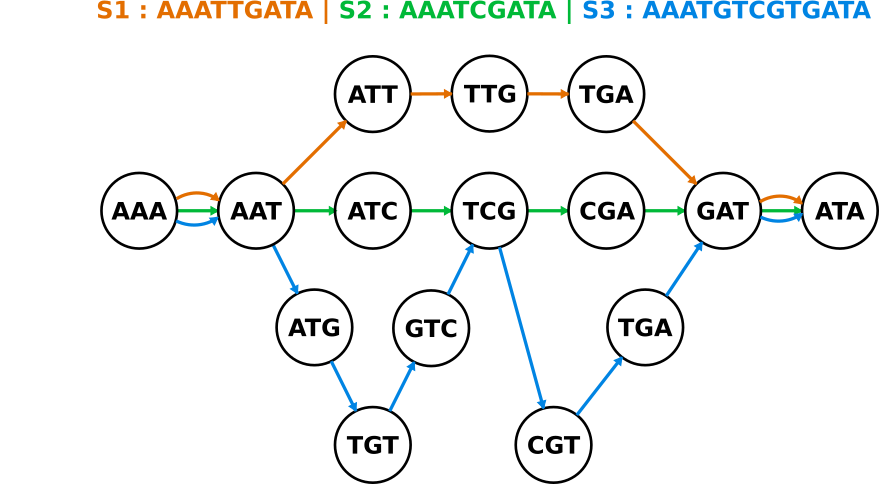
\includegraphics[width=.9\linewidth]{images/DBG.png}
    \caption[Exemple d'un graphe de De Bruijn]{\textbf{Exemple d'un graphe de De Bruijn.} Ici $k=3$, ce graphe permet de représenter et de reconstruire 3 séquences.}
    \label{fig:deBruijn}
\end{figure}

Les DBG, permettent d'avoir une structure compacte des séquences du pangénome. Les n\oe uds et les arêtes sont colorées en fonction des génomes dans lesquels ils sont retrouvés. Les DBG peuvent être compactés en cDBG, en fusionnant chaque région \textit{core}, \textit{i.e.} chaque suite de n\oe uds avec une seule arête entre chaque n\oe ud. Ces nouveaux n\oe uds fusionnés sont appelés "\textit{unitig"} et seront étiquetés avec la séquence combinée des k-mers.

L'une des premières méthodes développées utilisant des DBG est la méthode Cortex \cite{iqbal_novo_2012}, qui construit un DBG "coloré" (les arêtes et les n\oe uds sont étiquetés par les échantillons dans lesquels ils sont trouvés). À partir de ce DBG coloré, il est possible d'identifier les variants et de les associer à un génotype. Des outils plus récents, comme Bifrost \cite{holley_bifrost_2020}, améliorent les méthodes de coloration de DBG, permettant d'augmenter le volume de données pris en compte et supportant la mise à jour du graphe. Les auteurs de Bifrost ont notamment appliqué leur méthode sur une collection de plus de 100 000 génomes de \textit{Salmonella} \cite{luhmann_blastfrost_2021}, leur permettant d'identifier des gènes reliés à des îlots de pathogénicité et à une résistance aux fluoroquinolones\footnote{Classe d'antibiotique utilisée pour traiter les infections bactériennes graves.}.

\newpage
SplitMEM \cite{marcus_splitmem_2014}, permet de construire rapidement et efficacement des cDBG en intégrant une méthode appelée "saut de suffixe"\footnote{Le cDBG est relié à des arbres de suffixes, un saut de suffixe permet depuis un suffixe à l'extrémité d'une branche de l'arbre de sauté vers un même suffixe plus proche de la racine. Les sauts se poursuivent jusqu'à atteindre le suffixe le plus proche de la racine. Le chemin restant correspond au chemin le plus court sans ramification, entre la racine et le suffixe.}, qui permet de construire le cDBG sans passer par un DBG. L'outil permet ensuite de détecter dans l'ensemble des génomes ou dans un sous-ensemble de génomes les régions compressées (appelées \textit{Maximum Exact Matches} : MEMs), correspondant au \textit{core genome}. Cet outil est linéaire en temps et en espace pour identifier le \textit{core genome}, mais ne permet pas de mener d'autres analyses. De plus, la méthode a été testée sur un jeu de 62 génomes de \textit{E. coli}, le caractère linéaire est donc à vérifier sur de plus grands jeux de données.

PanTools \cite{sheikhizadeh_pantools_2016}, est un outil complet qui a largement évolué depuis sa publication. Il permet la construction de pangenomes basés sur des cDBG généralisés. PanTools est robuste à l'utilisation de grands volumes de données, que ce soit en temps, en mémoire ou en stockage. Il intègre également des méthodes d'annotation structurale et fonctionnelle, de partitionnement, d'alignement, de phylogénie, d'identification du \textit{core genome} et de visualisation. 

DBGWAS \cite{jaillard_fast_2018}, construit également les pangénomes avec des cDBG. Son originalité réside dans l'association de phénotypes (\textit{Genome Wild Association Study} : GWAS). L'intérêt d'utiliser le graphe de pangénome est qu'il n'est pas nécessaire d'utiliser une séquence de référence, contrairement aux approches classiques de GWAS. De plus, les phénotypes ne sont pas associés à des SNPs mais à des sous-graphes, permettant d'extraire des variants plus longs ou plus complexes. DBGWAS intègre une partie visualisation, permettant d'explorer les variants associés au phénotype dans leur contexte génomique pour identifier des régions variables plus larges comme les îlots génomiques. 

Le DBG (et ses dérivés) est une structure de données puissante, permettant de calculer, analyser et stocker, rapidement et efficacement, de grandes quantités de données. Néanmoins, ce qui fait la force de cette approche (l'utilisation de k-mer) est aussi sa faiblesse. Le choix de la taille du k-mer va influencer le graphe et donc la découverte des variations. De plus, cette structure est limitée dans l'identification et l'étude des régions répétées. C'est pourquoi des auteurs proposent des méthodes pour lier des informations au DBG \cite{turner_integrating_2018}.

\subsubsection{Application des graphes de pangénome.}

L'utilisation de pangénomes de séquence est très utile à partir de lectures courtes pour améliorer le génotypage. En utilisant le pangénome, contenant des variants connus, on améliore la couverture des lectures et donc on améliore le génotypage de ces lectures. Par rapport aux méthodes utilisant un génome de référence, le pangénome réduit le biais en faveur de la séquence de référence, particulièrement pour les grandes insertions/délétions et les SV. Le pangénome améliore aussi le \textit{variant calling} (VC) en augmentant sa précision, et à partir des DBG de faire du VC sans référence.

Les graphes de séquences sont également utilisés en métagénomique. L'outil MetaKallisto \cite{schaeffer_pseudoalignment_2017} utilise notamment une base de données de séquences représentantes qu'il représente sous forme de DBG coloré afin de faire de l'assignation taxonomique et de la quantification de séquences métagénomiques.

L'utilisation des graphes de séquences pour les GWAS permet de détecter finement des variations dans les populations associées à un phénotype. Chaguza \textit{et al.} \cite{chaguza_bacterial_2020} ont mené une étude sur 909 échantillons de souche hyper virulente de \textit{Streptococcus pneumoniae} (serotype 1). Ils ont pu identifier, grâce à l'outil DBGWAS, des mutations de certaines protéines associées à des phénotypes spécifiques (âge de l'hôte, géographie, structure des populations\dots). L'utilisation de graphes de pangénome a permis de mener une étude à large échelle, tout en prenant en compte toute la diversité sans nécessiter de référence.

\begin{table}[htbp]
    \centering
    \begin{tabular}{|p{.25\textwidth}|p{.3\textwidth}|p{.35\textwidth}|}
        \hline
        Nom & Méthode & Référence \\
        \hline
        NGSPanPipe & Séquence représentative & \cite{kulsum_ngspanpipe_2018} \\
        \hline
        Spine & Séquence représentative & \cite{ozer_characterization_2014}\\
        \hline
        VG toolkit & Variant prédéterminé & \cite{garrison_variation_2018} \\
        \hline
        Minigraph & Alignement sur graphe & \cite{li_design_2020} \\
        \hline
        PanVC & Variant prédéterminé & \cite{norri_founder_2021} \\
        \hline
        Minigraph-Cactus & MSA & \cite{hickey_pangenome_2024}\\
        \hline
        Harvest & MSA & \cite{treangen_harvest_2014} \\
        \hline
        PGGB & MSA & \cite{garrison_building_2024}\\
        \hline
        Cortex & graphe de De Bruijn & \cite{iqbal_novo_2012} \\
        \hline
        Bifrost & graphe de De Bruijn & \cite{holley_bifrost_2020} \\
        \hline
        SplitMEM & graphe de De Bruijn & \cite{marcus_splitmem_2014} \\
        \hline
        PanTools & graphe de De Bruijn & \cite{sheikhizadeh_pantools_2016} \\
        \hline
        twoPaCo & graphe de De Bruijn & \cite{minkin_twopaco_2017}\\
        \hline
        DBGWas & graphe de De Bruijn & \cite{jaillard_fast_2018}\\
        \hline
        PanVA & Visualisation & \cite{van_den_brandt_panva_2024} \\
        \hline
    \end{tabular}
    \caption[Outils de pangénomique basés sur les séquences]{\textbf{Liste non exhaustive d'outils de pangénomique basés sur les séquences.}}
    \label{tab:pangenomicToolsSeq}
\end{table}
\newpage
\section{Pangenome de gènes}

\subsection{Généralités et concepts}

Les outils basés sur des pangénomes de gènes, aussi appelés \textit{Presence-absence variation pangenome}s (en anglais, PAV), représentent une grande part des outils de pangénomique procaryote. Le génome des procaryotes étant majoritairement codant, et ce type de pangénome étant plus facile à manipuler et à interpréter, de nombreuses études utilisent les gènes comme unité pour construire les pangénomes. Pour construire ces pangénomes, on commence par regrouper les gènes en familles de gènes, puis on partitionne\footnote{N.B : Dans la suite, pour ne pas faire de confusion entre le partitionnement des familles et le partitionnement des gènes en famille de gènes, nous utiliserons le terme clustering pour parler de la construction des familles de gènes.} les familles en fonction de leur présence dans les génomes (\textit{core}, \textit{accessory}\dots).

% \newpage
\paragraph{Construction des familles de gènes}

La construction des familles de gènes consiste à appliquer une méthode de clustering des gènes par similarité, que nous avons vue en \autoref{sec:clustering}. Le choix de la méthode et des seuils appliqués dans le clustering auront un impact important sur le pangénome. L'outil de clustering influencera aussi l'interprétation. Tout d’abord, les outils d’analyse peuvent s’appuyer sur différents niveaux d’information, tels que la séquence nucléotidique ou protéique, la structure tridimensionnelle des protéines ou encore la fonction biologique associée. Le choix de cette base de comparaison influence de manière déterminante le calcul de la similarité, et par extension, l’inférence du caractère homologue. De plus, en utilisant un outil qui construit des clusters (et donc des familles) d'orthologues, comme orthoMCL \cite{li_orthomcl_2003} ou la base de données COG (cluster of orthologous genes), on retrouvera dans la même famille les gènes ayant suivi les mêmes événements de spéciation. Si l'outil permet de différencier les paralogues des orthologues comme InParanoïd \cite{remm_automatic_2001}, il y aura plus de familles que si on prenait en compte uniquement l'homologie. Le choix de la méthode de clustering est donc essentiel.

\paragraph{Partitionnement du pangénome}

Une fois que les génomes ont été annotés et les familles de gènes construites, les familles de gènes sont partitionnées en fonction de leur présence/absence dans les génomes. Dans les premières analyses, les familles étaient séparées en 2 parties (\autoref{fig:pangenome2}), les familles qui sont présentes dans tous les génomes sont dites "c\oe ur" (\textit{core} en anglais) et les autres sont dites "accessoire" (\textit{accessory} ou \textit{dispensable} en anglais). Cette dichotomie en \textit{core genome} et \textit{accessory genome} est liée au caractère essentiel ou non des fonctions codées par les gènes. Les familles "\textit{core}" sont impliquées dans les processus cellulaires vitaux, ce qui crée une forte pression de sélection de leurs gènes et une forte conservation dans l'ensemble des génomes. À l'inverse, les familles accessoires sont plutôt liées à des adaptations à l'environnement, à un mode de vie\dots. Leurs gènes sont donc moins soumis à la pression de sélection et donc moins conservés dans les génomes.

\begin{figure}[htbp]
    \centering
    \subfloat[Pangénome bipartie]{
        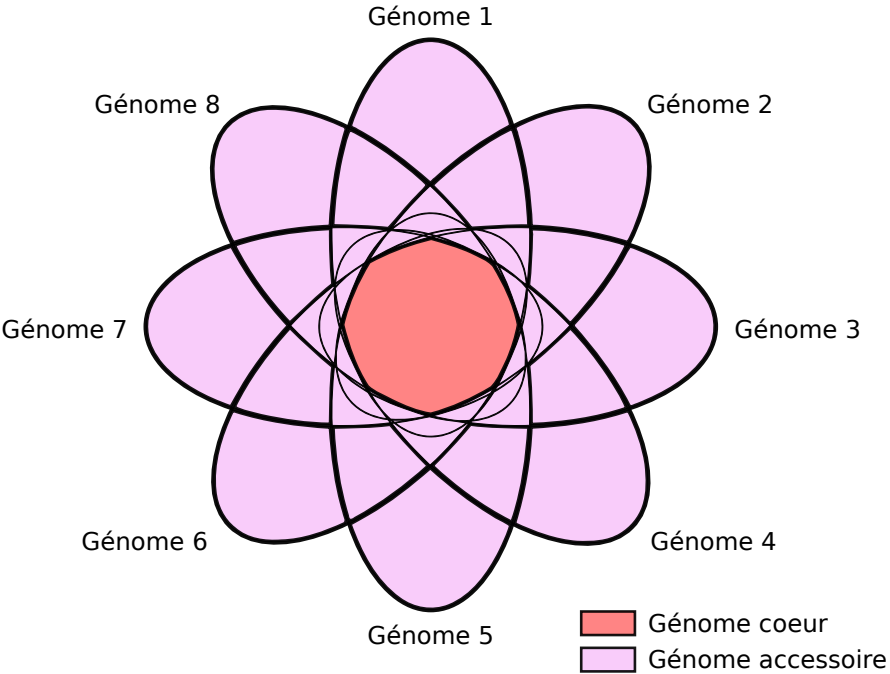
\includegraphics[width=0.48\linewidth]{images/pangenome2.png}
        \label{fig:pangenome2}
    }
    \hfill
    \subfloat[Pangénome tripartie]{
        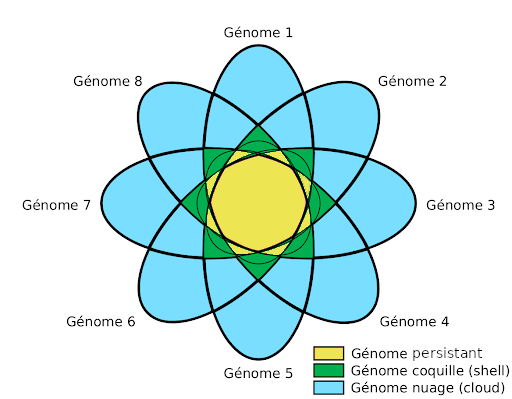
\includegraphics[width=0.48\linewidth]{images/pangenome3.png}
        \label{fig:pangenome3}
    }
    \caption[Partitionnement des pangénomes.]{\textbf{Partitionnement des pangénomes.} Extrait et adapté de \cite{gautreau_conceptualisation_2020}}
    \label{fig:pangenomeVenn}
\end{figure}

\newpage
Ce partitionnement du pangénome en 2 parties, bien que largement utilisé, est une vision très limitée de la distribution des gènes dans les génomes, qui peut amener à des erreurs d'interprétation. Il faut d'abord prendre en compte que même si le nombre de génomes disponibles est de plus en plus conséquent, il n'est toutefois pas possible d'avoir l'ensemble des génomes d'une espèce (cf. \autoref{sec:croissance_pan}), ce qui implique qu'il est plus que probable que des gènes soient identifiés comme accessoires alors qu'ils sont \textit{core} et inversement. 
De plus, les techniques de séquençage et les outils bioinformatiques ne sont pas infaillibles, et donc une erreur d'assemblage, d'annotation, de regroupement en familles, ou encore l'utilisation de génomes partiels, peut entraîner le mauvais classement d'une famille. Pour répondre à ce problème, Lapierre et Gogarten \cite{lapierre_estimating_2009} suggèrent de définir un c\oe ur relâché (\textit{soft-core} en anglais), qui contient les familles présentes dans 95 \% des génomes\footnote{ce pourcentage peut varier en fonction des études.}. Une autre proposition, de Snippen \textit{et al.} \cite{snipen_microbial_2009} raffinant un modèle proposé par Hogg \textit{et al.} \cite{hogg_characterization_2007}, rendrait le nombre de partitions variable en fonction du contenu du pangénome. Cette dernière proposition permet de ne pas utiliser de seuil fixe pour partitionner les familles.
En parallèle, Koonin \textit{et al.}, dans une analyse de l'ensemble des génomes procaryotes disponibles en 2008 \cite{koonin_genomics_2008}, et Makarova \textit{et al.}, en étudiant l'ensemble des génomes d'archées disponibles en 2007 \cite{makarova_clusters_2007}, proposent une vision tripartie du pangénome (\autoref{fig:pangenome3}). Les 2 articles suivent une méthodologie similaire : après une annotation fonctionnelle des génomes, ils comptabilisent le nombre de génomes associés à chaque fonction (COGs pour Makarova et EggNOGs \cite{jensen_eggnog_2008} pour Koonin). Les résultats obtenus révèlent une distribution en forme de courbe en U, où chaque extrémité correspond à une catégorie spécifique de fonctions, tandis que la base regroupe une autre catégorie distincte. Ils redéfinissent alors le core genome comme l’ensemble des gènes présents dans la quasi-totalité des génomes. Ce \textit{core genome} relâché et flexible (sans seuil) est aussi appelé \textit{soft-core genome}, ou encore \textit{persistent genome}, dans certains articles pour le différencier du \textit{core genome} strict défini en premier. L'\textit{accessory genome} sera lui divisé en 2, le \textit{cloud genome} correspondant aux gènes partagés par un faible nombre de génomes, et le \textit{shell genome} correspondant aux gènes ayant une fréquence intermédiaire dans les génomes. Ces différents partitionnements, qui ne sont pas incompatibles, sont de plus en plus utilisés, dû au nombre croissant de génomes disponibles. 

\paragraph{Modélisation et représentation des pangénomes de gènes}

Pour représenter les pangénomes de gènes, il est possible d'utiliser une matrice de présence/absence des gènes (\autoref{fig:panType}B). Cette représentation permet de rapidement identifier le \textit{core genome} ou de trouver les gènes spécifiques à un génome d'intérêt par exemple. Une seconde représentation est celle du diagramme de Venn (\autoref{fig:pangenomeVenn}). À partir du diagramme, on peut rapidement avoir une idée de la proportion de chaque partie, et aussi de la "croissance" du pangénome. Ces 2 représentations ont l'intérêt d'être simples à calculer et à interpréter, néanmoins, lorsque le nombre de génomes devient trop important, il n'est plus possible de les visualiser correctement. De plus, elles se focalisent exclusivement sur le contenu en gènes des génomes, sans fournir d’informations sur leur arrangement ou leur structure organisationnelle.

Afin d’intégrer l’organisation des gènes en plus de leur simple présence, une approche alternative repose sur une représentation où les gènes et leurs relations sont modélisés sous forme de graphe. Dans ce graphe, les familles de gènes constituent les n\oe uds et les relations de voisinage entre les gènes correspondent aux arêtes. Sur la \autoref{fig:graphPanFam}, on peut voir que dans cette représentation, plus les familles ont des gènes voisins, plus le poids de l'arête (épaisseur) augmente. Le graphe de pangénome permet alors d'identifier des structures ou des chemins de familles conservées, ou à l'inverse des régions fortement variables.

\begin{figure}[htbp]
    \centering
    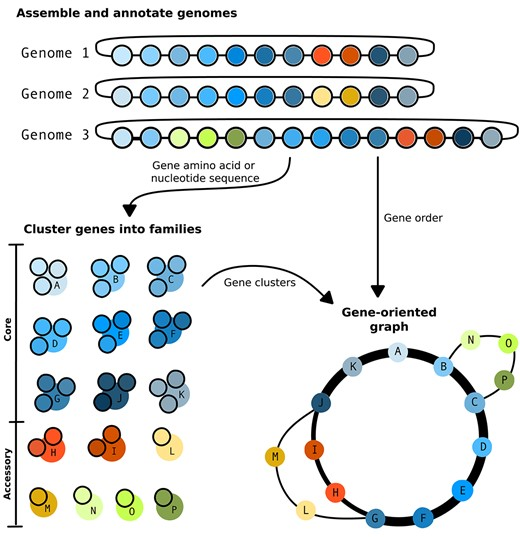
\includegraphics[width=0.8\linewidth]{images/graphePanFam.jpeg}
    \caption[Représentation d'un pangénome de gènes sous forme de graphe]{\textbf{Représentation d'un pangénome de gènes sous forme de graphe.} Extrait de \cite{matthews_gentle_2024}}
    \label{fig:graphPanFam}
\end{figure}

\subsection{Méthodes et outils de pangénome de gènes}

Le premier outil dédié à la construction de pangénomes de famille de gènes est Edgar \cite{blom_edgar_2009}. Disponible en ligne, ce n'est pas un outil à proprement parler, mais plutôt une ressource de résultats d'analyse de pangénome. Dans sa méthode, Edgar clusterise les gènes en familles d'orthologues, en utilisant le BBH\footnote{\textit{Bidirectional Best Hit}}. Les génomes étant relativement proches dans les analyses, les paralogues récents pourraient être regroupés avec des orthologues. Les familles sont donc raffinées en utilisant un système de score pour valider les BBH. Dans sa version actuelle, l'outil permet d'identifier le \textit{core genome} et l'\textit{accessory genome}, rechercher des synténies conservées, de construire des arbres phylogénétiques, ou encore d'annoter fonctionnellement les gènes à partir de bases de données de référence.

Le premier outil permettant la construction de pangénome en ligne de commande est PGAP \cite{zhao_pgap_2012}. Le premier intérêt de PGAP, est qu'il permet à l'utilisateur de construire un pangénome avec ses propres génomes. PGAP construit lui aussi des familles d'orthologues. À partir de ces familles, il propose différentes analyses, comme la courbe de raréfaction, le profil du pangénome\footnote{Le nombre de gènes (y) présents dans x génomes.}, l'identification du \textit{core genome}, l'analyse de variants. Une interface PGAP-X \cite{zhao_pgap-x_2018} rend l'outil plus accessible et améliore la visualisation des résultats.

PanOCT \cite{fouts_panoct_2012} est un autre outil disponible en ligne de commande. Il propose aussi un clustering en famille orthologues, similaire à EDGAR, mais améliore l'algorithme en ajoutant l'information de contexte conservé (\textit{Conserved Gene Neighborhood}, CGN). Les gènes orthologues ont tendance à conserver leur organisation génomique dans les espèces proches contrairement aux espèces éloignées et aux gènes paralogues \cite{huynen_measuring_1998,rocha_organization_2008}. En combinant le BBH et le CGN, les familles de gènes orthologues sont de meilleure qualité. L'outil PanACEA \cite{clarke_panacea_2018} récupère les familles de PanOCT et permet de visualiser le pangénome, mais aussi de l'annoter, notamment avec des informations liées à l'antibiorésistance. 

PanFunPro \cite{lukjancenko_panfunpro_2013}, propose une méthode originale pour construire des familles de gènes homologues, en se basant sur l'annotation fonctionnelle des protéines. Pour annoter les protéines, il utilise des profils HMM de différentes bases de données de domaines protéiques. En définissant l’homologie selon la fonction plutôt que la séquence, cette approche propose un cadre d’analyse alternatif, privilégiant les similarités fonctionnelles des protéines et offrant ainsi une vision complémentaire aux méthodes traditionnelles.

Roary \cite{page_roary_2015} est l'outil de pangénomique certainement le plus utilisé et le plus célèbre. Sa popularité vient de sa capacité à générer des pangénomes de façon rapide en demandant peu de ressources par rapport à ses concurrents de l'époque. Pour ça, il utilise un algorithme CD-Hit pour grouper les séquences proches avant d'aligner les séquences représentantes entre elles avec BLASTP. Les familles sont construites avec l'algorithme MCL et raffinées en utilisant les informations de colocalisation. Roary est aussi un des premiers programmes à représenter les pangénomes de gènes sous forme d'un graphe dans lequel les n\oe uds sont les gènes et les arêtes représentent une relation de voisinage dans les génomes.

\newpage
D'autres outils vont reprendre ce modèle de graphe de gènes, comme Panaroo \cite{tonkin-hill_producing_2020}. À partir du graphe, il corrige les erreurs d'annotation et d'assemblage. Il dispose également de plusieurs modules d'analyse : GWAS, SV, phylogénie et visualisation du pangénome. Panaroo est un outil performant, mais demande des ressources de calcul relativement importantes et une expertise bioinformatique plus importante que d'autres outils. De plus, en nettoyant le graphe, il est possible qu'il élimine des évènements évolutifs récents, et donc ne pas être adapté à des taxons dans lesquels les taux de HGT sont élevés par exemple. Panakeia \cite{beier_panakeia_2022} est un outil reposant aussi sur un modèle de graphe de pangénome, mais propose une analyse plus "universelle". L'outil propose entre autres l'identification de chemins particuliers dans le graphe, correspondant à des structures biologiques, comme les îlots génomiques.

Les outils présentés jusqu'ici, bien que non limités théoriquement, sont généralement appliqués à la construction de pangénomes au niveau de l'espèce. Des méthodes, comme RIBAP \cite{lamkiewicz_ribap_2024}, proposent de construire des pangénomes au niveau du genre. RIBAP construit un pangénome en utilisant ROARY à 95 \% d'identité. En parallèle, il utilise MMSeqs2 pour aligner l'ensemble des gènes. Le résultat de l'alignement est ensuite utilisé pour raffiner les familles pour construire des familles homologues au niveau du genre. De cette manière, la partie de \textit{core genome} est plus importante. Avec ce nouveau partitionnement, RIBAP propose de construire un arbre phylogénétique des souches présentes dans le pangénome. 

L'utilisation de pangénomes de gènes est bien adaptée à la génomique comparée des procaryotes. Leur simplicité de calcul et d'interprétation les rend accessibles pour tous les utilisateurs. Néanmoins, cette simplicité est liée à une vision gène centrée, qui ne prend pas en compte les régions non codantes. Des outils, comme Piggy \cite{thorpe_piggy_2018}, permettent de pallier ce problème en proposant une analyse complémentaire à un pangénome de gène généré par Roary. Ainsi, la complémentarité des outils permet d'avoir une étude plus complète. 

En 2020, PPanGGOLiN \cite{gautreau_ppanggolin_2020} introduit une stratégie de partitionnement, s’appuyant sur un algorithme de \textit{machine learning} pour classifier les gènes du pangenome. Cette approche repose sur une analyse des relations de voisinage et du clustering, éliminant ainsi la nécessité de fixer des seuils stricts. Par conséquent, PPanGGOLiN permet d’identifier de manière dynamique les trois composantes du pangenome — \textit{persistent genome}, \textit{shell genome} et \textit{cloud genome} — sans présupposer de leur répartition.

\subsection{Analyses à partir de pangénomes de gènes}

Les pangénomes de gènes sont utilisés pour mener des études de phylogénomique. En 2020, Gaba \textit{et al.} \cite{gaba_pan-genome_2020} s'intéressent aux archées de la classe des Halobacteria, des archées extrêmement halophiles\footnote{Capable de vivre dans des milieux à haute concentration en sel}. Ils vont construire un pangénome à l'aide de l'outil GET\textunderscore HOMOLOGUE \cite{contreras-moreira_get_homologues_2013}, un outil similaire à EDGAR. À partir de ce pangénome, ils ont pu identifier les gènes \textit{core} des gènes \textit{accessory}. Sur la base de ce partitionnement, ils ont pu mettre en évidence un fort taux de transferts horizontaux au sein de la classe des Halobacteria. Ils ont alors construit une phylogénie basée sur le pangénome et sa partition, mettant en évidence une évolution étroite entre l'ordre des Natrialbales et celui des Halobacteriales, suggérant alors l'existence d'un superordre les regroupant. Plusieurs méthodes permettent d’ailleurs d'identifier les régions où les transferts horizontaux de gènes se produisent préférentiellement. Parmi elles, la méthode panRGP\cite{bazin_panrgp_2020} permet de détecter les régions de plasticité génomique (RGP), \textit{i.e.} des segments du génome échangés entre différentes souches par transfert horizontal ou perdus de manière différentielle selon les lignées. Cette approche repose sur l’analyse du graphe de pangénome et de sa partition pour identifier les régions variables. Elle permet également d’identifier des spots, en repérant les familles de gènes persistantes flanquant les RGP. Une autre méthode, panModule\cite{bazin_panmodule_2021}, vise quant à elle à détecter des groupes de familles de gènes variables dans le pangénome, qui sont organisés en blocs de synténie au sein des génomes. Ces deux méthodes sont intégrées à la suite logicielle PPanGGOLiN et exploitent le graphe de pangénome généré par cette dernière.

Dans les exemples cités, les études étaient centrées sur des groupes taxonomiques et donc les génomes appartenaient au même taxon. Pourtant, comme nous l'avons déjà vu, l'étude d'environnements et les données métagénomiques sont étroitement liées aux études pangénomiques. Vera-Ponce de León \textit{et al.} \cite{vera-ponce_de_leon_genomic_2024}, produisent un atlas génomique du microbiote des saumons. Pour caractériser les espèces présentes et construire le pangénome, ils utilisent l'outil mOTUpan \cite{buck_motupan_2022}. mOTUpan permet de clusteriser les métagénomes à un fort niveau d'identité (95 \%), définissant ainsi des unités taxonomiques opérationnelles métagénomiques (mOTUs, \textit{metagenomic Operational Taxonomic Unit} en anglais). Chaque mOTU peut être associé à une espèce (ou un taxon) et donc permettre de séparer les gènes appartenant à la même espèce dans une même mOTU. L'intérêt de mOTUpan est qu'il utilise un modèle bayésien pour estimer le génome \textit{core} et le génome accessoire. Ce modèle prend en compte la complétion (souvent faible) des métagénomes et améliore la qualité du partitionnement sur ces données. À partir du pangénome, les auteurs ont pu identifier 14 ordres bactériens différents, représentant 35 genres distincts, ils ont également identifié 29 nouvelles espèces encore non répertoriées.

Les méthodes de machine learning peuvent aussi être utilisées pour analyser les pangénomes. Dans leur article, Kavvas \textit{et al.} \cite{kavvas_machine_2018} proposent d'utiliser des méthodes de machine learning pour identifier des gènes de résistance aux antibiotiques dans 1 595 souches de \textit{Mycobacterium tuberculosis}. Le pangénome est construit à partir de familles homologues, et les gènes connus pour être des gènes de résistance aux antibiotiques sont annotés. En utilisant des méthodes de machine learning (SVM, MI, ANOVA\dots), les auteurs ont pu identifier 24 nouveaux gènes de résistance, de plus le signal de certains gènes déjà connus est plus fort que mesuré précédemment. Les auteurs ont poursuivi en analysant la structure des nouveaux gènes et de leurs protéines, ainsi qu'en menant une étude géographique de la répartition des gènes pour établir des liens entre population hôte et résistance. Il faut néanmoins rappeler une nouvelle fois que la découverte de ces nouveaux gènes doit être vérifiée et que leur identification n'est possible que sur la base d'une base de données de gènes connus.

\begin{table}[htbp]
  \centering
  \footnotesize
  \begin{tabular}{|p{.2\textwidth}|p{.38\textwidth}|p{.35\textwidth}|}
    \hline
    Nom & Méthode & Référence \\
    \hline
    EDGAR & matrice présence/abscence & \cite{blom_edgar_2009}\\
    \hline
    PGAP & matrice présence/abscence & \cite{zhao_pgap_2012}\\
    \hline
    PanOCT & Clustering d'orthologue & \cite{fouts_panoct_2012}\\
    \hline
    GET\textunderscore HOMOLOGUES & Clustering d'orthologue & \cite{contreras-moreira_get_homologues_2013} \\
    \hline
    PanACEA & Visualisation & \cite{clarke_panacea_2018}\\
    \hline
    PanFunPro & Familles de profil fonctionnelle & \cite{lukjancenko_panfunpro_2013}\\
    \hline
    Roary & Graphe de famille de gène & \cite{page_roary_2015}\\
    \hline
    Piggy & Analyse région intergénique & \cite{thorpe_piggy_2018}\\
    \hline
    Ptolemy & Graphe de famille de gène & \cite{thorpe_piggy_2018}\\
    \hline
    PIRATE & Graphe de famille de gène & \cite{bayliss_pirate_2019}\\
    \hline
    Panaroo & Graphe de famille de gène & \cite{tonkin-hill_producing_2020}\\
    \hline
    PPanGGOLiN & Graphe de famille de gène & \cite{gautreau_ppanggolin_2020}\\
    \hline
    PanACoTA & Graphe \& Phylogénie & \cite{perrin_panacota_2021} \\
    \hline
    Panakeia & Graphe de famille de gène & \cite{beier_panakeia_2022}\\
    \hline
    PanPhlAn & Graphe de données métagénomique & \cite{scholz_strain-level_2016}\\
    \hline
    MSPminer & Graphe de données métagénomique & \cite{plaza_onate_mspminer_2019}\\
    \hline
    mOTUpan & Graphe de données métagénomique & \cite{buck_motupan_2022}\\
    \hline
    Pan-Tetris & Visualisation & \cite{hennig_pan-tetris_2015}\\
    \hline
    PanViz & Visualisation & \cite{pedersen_panviz_2017}\\
    \hline
    Panache & Visualisation & \cite{durant_panache_2021}\\
    \hline
    
  \end{tabular}
  \caption[Outils de pangénomique basés sur les familles de gènes]{\textbf{Liste non exhaustive d'outils de pangénomique basés sur les familles de gènes}}
  \label{tab:pangenomicToolsFam}
\end{table}

\newpage
\section{Conclusion sur les pangénomes et éléments de réflexions}

Nous avons présenté une grande variété de méthodes et d'outils de pangénomique (\textit{cf.} tableaux \ref{tab:pangenomicToolsSeq} et \ref{tab:pangenomicToolsFam}) et exploré plusieurs champs d'application des pangénomes. Cependant, plusieurs défis majeurs restent à relever en pangénomique.

Un premier défi concerne la représentation et la visualisation des pangénomes. En effet, ceux-ci doivent être visualisables par l'\oe il humain tout en intégrant l’ensemble de l’information génomique. Différentes approches ont été développées pour répondre à cette problématique, notamment des outils de visualisation interactifs. À titre d’exemple, Pan-Tetris\cite{hennig_pan-tetris_2015} permet de visualiser et de modifier la composition des groupes de gènes grâce à une technique inspirée du jeu Tetris. PanViz\cite{pedersen_panviz_2017} facilite la comparaison des génomes individuels aux pangénomes avec une navigation basée sur l'ontologie des gènes. PanVa\cite{van_den_brandt_panva_2024}, utilisant les pangénomes de PanTools\cite{sheikhizadeh_pantools_2016}, propose une approche centrée sur la variabilité structurale, permettant une analyse flexible des pangénomes en tenant compte des variations génomiques complexes. Enfin, PANACHE\cite{durant_panache_2021} propose une visualisation linéarisée des pangénomes, affichant la présence ou l’absence des blocs de séquences sous forme de navigateur génomique.

Un second défi crucial est celui du stockage et de la gestion des données pangénomiques. Contrairement aux génomes individuels, généralement stockés sous forme de texte et reliés à des bases de données, les pangénomes sont des structures plus complexes qui ne peuvent être stockées sous un format linéaire. Les BD doivent donc permettre un accès rapide et efficace aux informations, tout en étant mises à jour régulièrement pour suivre l’augmentation du volume des données génomiques. Des BD comme panKB \cite{sun_pankb_2025}, permettent d'avoir accès à des informations sur des pangénomes précalculés, reliés à des métadonnées comme : les publications de référence, les informations sur l'origine des génomes\dots 
Cependant, le pangénome en lui-même n'est pas disponible et seuls les résultats d'analyse sont disponibles.

Enfin, un défi essentiel concerne la construction du pangénome. Le choix des méthodes influence fortement le résultat final, mais les données d’entrée jouent également un rôle fondamental. L’objectif étant de représenter au mieux la diversité génomique, il est important de maximiser cette diversité tout en évitant les biais, tels que la surreprésentation de génomes pathogènes dans les bases de données. Un équilibre est nécessaire : trop de variations dans les données d’entrée peuvent complexifier l’analyse, en rendant par exemple les graphes de pangénome difficilement exploitables. La qualité des génomes, des annotations et des bases de données, sont également des facteurs déterminants pour garantir la robustesse des analyses pangénomiques.

Pour répondre à ces défis, les méthodes et les outils de pangénomique sont en constante évolution. Avec ces progrès, divers domaines de la microbiologie voient progressivement s'intégrer des analyses pangénomiques en routine. Cette intégration repose en partie sur des plateformes qui rendent ces outils accessibles et exploitables par la communauté scientifique. Par exemple, MicroScope\cite{vallenet_microscope_2020} permet de construire des pangénomes procaryotes à l’aide de PPanGGOLiN \cite{gautreau_ppanggolin_2020} et d’identifier les régions de plasticité génomique (RGP) grâce à la méthode panRGP\cite{bazin_panrgp_2020}. MicroScope constitue alors un point d'intersection entre les données génomiques, la production de pangénomes et leur utilisation effective, contribuant ainsi à relever progressivement les défis liés à la visualisation, au stockage et à la construction des pangénomes.
\chapter{Génomique à l'ère du BigData}
\section{Base de données génomiques : ressources et exploitation}
\label{sec:db}
\section{La pangénomique}
\section{Base de données orienté graphe et données biologiques}
\part{Du génome au pangénome}
\part{De la génomique comparée à la pangénomique comparée}
\label{part:PANORAMA}

Avec l’augmentation du nombre de génomes disponibles, les approches traditionnelles basées sur l’analyse de génomes individuels montrent leurs limites. Le concept du pangénome s'est peu à peu imposé et la construction de graphes est de plus en plus répandue pour étudier leur diversité génétique. Il est désormais possible de générer un grand nombre de pangénomes, offrant pour chaque espèce une vision complète de la variabilité génétique. La comparaison de ces pangénomes offre alors l’opportunité d’identifier leurs similarités et spécificités respectives, en considérant simultanément l’ensemble des gènes.

Dans cette perspective, nous avons développé PANORAMA, un outil dédié à l’intégration de méthodes de pangénomique comparée, facilitant ainsi l’analyse systématique des variations génétiques inter-pangénomiques.

\chapter{PANORAMA : un nouvel outil pour la pangénomique comparée}
\section{Prédiction des systèmes biologiques dans les pangénomes}

L’annotation des pangénomes est essentielle pour donner du sens aux analyses pangénomiques, que ce soit le partitionnement, la recherche de structures (comme les modules) ou des arbres phylogénétiques. Certains outils, tels que Panaroo \cite{tonkin-hill_producing_2020} et PanTools \cite{sheikhizadeh_pantools_2016}, offrent la possibilité d’importer des annotations externes directement dans le graphe de pangénome. D’autres, comme PanGraph \cite{noll_pangraph_2023}, intègrent des méthodes d’alignement des éléments du pangénome (gènes ou familles de gènes) sur des bases de données fonctionnelles. PPanGGOLiN, quant à lui, intègre ces deux approches en ajoutant des métadonnées à tous les éléments du pangénome et en proposant une commande permettant d’aligner les séquences pangénomiques sur une base de données externe.

Toutefois, ces approches se limitent à l’annotation des gènes ou des familles de gènes, à l’exception des métadonnées intégrées dans PPanGGOLiN. À ce jour, aucune méthode ne permet, à notre connaissance, d’identifier des structures fonctionnelles plus complexes, telles que des systèmes biologiques, dans le graphe de pangénome.

La prédiction de systèmes biologiques dans les données génomiques, en particulier chez les procaryotes, repose sur un large éventail d’outils et de méthodes (\textit{cf.} \autoref{sec:sys_bio}). Cependant, ces approches sont centrées sur le génome individuel et ne prennent pas en compte l’ensemble de la diversité génétique de l'espèce. Or, intégrer cette diversité est crucial pour mieux comprendre l’évolution et le rôle fonctionnel de ces systèmes.

Afin de pallier cette limitation, j’ai développé PANORAMA, un outil de pangénomique conçu pour prédire des systèmes biologiques dans les graphes de pangénome générés avec PPanGGOLiN. Cette méthode repose sur 2 points clés : (\textit{i}) Des modèles, similaires à ceux de MacSyFinder \cite{abby_macsyfinder_2014}, définissant des règles de présence/absence des gènes et leur organisation en synténie ;(\textit{ii}) une adaptation de la méthode de détection des contextes génomiques que j'ai développée dans PPanGGOLiN.

\section{Comparaison des pangénomes}

La majorité des études pangénomiques se concentrent sur la diversité génétique au sein d’une espèce ou d’un environnement donné. Bien que certaines recherches explorent le pangénome à des rangs taxonomiques supérieurs \cite{moulana_selection_2020}, les études comparant plusieurs pangénomes pour analyser la diversité entre différentes espèces procaryotes restent rares.

\newpage

Parmi les quelques travaux existants, C. Hyun \textit{et al.} \cite{hyun_comparative_2022} ont proposé une analyse comparative du pangénome de 12 espèces bactériennes pathogènes. Toutefois, leur approche ne repose pas sur le graphe de pangénome, mais sur la présence/absence des familles de gènes homologues dans les génomes. Leur étude se limite à la comparaison de certaines métriques associées aux pangénomes (telles que l’ouverture ou la loi de Heaps) ainsi qu’à l’annotation des familles de gènes.

À ce jour, cette analyse manuelle et spécifique à un jeu de données particulier semble être la seule existante  qui compare des pangénomes. Aucun outil pangénomique ne permet encore une comparaison automatique et non spécifique de plusieurs graphes de pangénomes afin d’identifier des structures conservées ou spécifiques.

Dans cette optique, j’ai intégré dans PANORAMA de nouvelles méthodes exploitant le graphe de pangénome ainsi que la composition en familles de gènes de structures telles que les spots, les modules ou les systèmes. Ces méthodes permettent de rechercher des éléments conservés entre plusieurs pangénomes. À notre connaissance, PANORAMA est le premier outil offrant une comparaison automatisée de graphes de pangénome, ouvrant ainsi la voie à une meilleure compréhension de la diversité métabolique et de la dynamique évolutive des génomes procaryotes.

\chapter{Article : PANORAMA}

\includepdf[pages=1-23]{Comparaison/PANORAMA_paper.pdf}

\chapter{Conclusion et perspectives}

\section{Prédiction de systèmes biologiques}

Le développement de PANORAMA représente une nouvelle avancée pour l'analyse des pangénomes procaryotes, en proposant une approche pour l'identification des systèmes biologiques. Contrairement aux méthodes traditionnelles qui reposent principalement sur l’annotation de gènes individuels, PANORAMA exploite directement le graphe de pangénome, prenant ainsi en compte la diversité globale des génomes. La méthode de prédiction repose sur l'utilisation d’une base de données HMM et d’un ensemble de modèles spécifiques, permettant d’identifier et de contextualiser les systèmes biologiques.

En exploitant les pangénomes générés par PPanGGOLiN, il devient possible d’associer ces systèmes aux RGPs, aux spots et aux modules, ce qui enrichit l’annotation réciproque de ces éléments. L’utilisation du pangénome permet également d’identifier des systèmes autrement inaccessibles aux méthodes classiques, notamment en permettant l’annotation des fragments de gènes à partir des familles. De plus, cette approche permet la détection de systèmes "fractionnés", \textit{i.e.} des systèmes dont les composants ne sont pas colocalisés dans un même génome, en raison d’insertions génomiques ou de leur position en bordure de contigs.

Dans la modélisation des systèmes, nous avons introduit un nouveau niveau de description, en regroupant les familles de gènes en unités fonctionnelles, ce qui améliore la caractérisation des modèles. PANORAMA ne possède pas de modèle propre, mais il permet de traduire des modèles issus de plusieurs bases de données existantes, telles que PADLOC, DefenseFinder et MacSyModels. Toutefois, la conversion entre ces bases n’est pas triviale : certaines différences dans les paramètres peuvent rendre la correspondance complexe, voire impossible. Néanmoins, la grammaire choisie et la lecture des modèles sont suffisamment simples et flexibles pour permettre l'écriture manuelle de modèles, et donc l'intégration de bases de données de systèmes propres et spécifiques. 

Nous prévoyons d’étendre cette approche à d’autres bases, comme les modules métaboliques de la base de données KEGG \cite{kanehisa_kegg_2025}. Ces modèles sont représentés sous une \textbf{forme normale disjonctive} (FND), qui utilise uniquement les opérateurs logiques \textit{et}, \textit{ou} et \textit{non} (ce dernier ne pouvant s’appliquer qu’à un élément isolé). Si cette grammaire était standardisée à toutes les BD de systèmes, cela faciliterait les conversions entre bases et permettrait l’automatisation des traductions. De plus, elle ouvrirait la possibilité d’optimiser les expressions en appliquant des algorithmes classiques de minimisation, rendant ainsi la recherche de systèmes plus efficace. Toutefois, la FND présente certaines limites : elle ne prend pas en compte des paramètres quantitatifs comme la transitivité ou les règles de \textit{quorum} et, dans le cas de modèles complexes, elle peut générer des expressions de taille exponentielle, difficiles à interpréter.

\newpage

Nous avons testé PANORAMA sur plusieurs bases de données, en particulier sur les modèles de défense contre les phages, où la méthode a démontré sa robustesse et son efficacité. Cependant, son application à d’autres modèles, comme ceux de conjugaison de MacSyFinder, a révélé certaines limites. Par exemple, une valeur élevée de transitivité (500 dans le modèle \textit{T4SS\_typeB} des plasmides) entraîne un goulot d’étranglement algorithmique. Cette difficulté provient d’une recherche de contexte extrêmement complexe, générant un graphe avec un nombre d’arêtes considérable, nécessitant ensuite un filtrage intensif. L’algorithme actuel n’est pas conçu pour traiter de telles valeurs. Une solution envisageable serait de distinguer les familles en unités fonctionnelles distinctes et d’introduire un mot-clé spécifique qui ne reconstruirait pas directement le contexte entre ces unités, mais se limiterait à rechercher un chemin d’une taille correspondant à la transitivité spécifiée.

\section{Comparaison de pangénomes}

PANORAMA ouvre également la voie aux approches de pangénomique comparée. En recherchant et comparant des structures identifiées dans les graphes de pangénome, PANORAMA peut extraire les éléments conservés ou spécifiques à certains groupes d’organismes. Il devient alors possible d’identifier des liens évolutifs, de détecter des modules fonctionnels partagés et d’étudier l’émergence ou la disparition de systèmes biologiques, en prenant en compte toute la diversité génomique. Cette capacité à comparer les graphes de pangénomes offre un nouveau cadre d’analyse pour mieux comprendre l’évolution et l’organisation des génomes chez les procaryotes.

Pour ce faire, notre méthode repose sur un score (GFRR) permettant d’évaluer la similarité en contenu en famille de gènes entre les éléments des pangénomes. Ces éléments doivent au préalable être détectés au sein du pangénome afin d’assurer la robustesse de la comparaison. L’identification de structures conservées, \textit{i.e.} des ensembles de familles de gènes partageant une organisation pangénomique similaire, reste un défi en cours d’exploration. Une piste repose sur l’application de méthodes de \textit{machine learning}. En s’appuyant sur des modèles entraînés sur des structures connues, il serait possible de détecter et de classifier de nouvelles régions d’intérêt, ouvrant ainsi la voie à la prédiction de structures conservées inédites entre différentes espèces.


L'ensemble des développements méthodologique de PANORAMA ont pu être présentés dans plusieurs conférences, sous forme de \textit{talk} et de poster (\textit{cf.} Annexes \ref{Ann:Communication}). Un article présentant PANORAMA sera prochainement soumis.
\part{Base de données de graphe de pangénomes}
\label{part:DBpan}
\chapter{Intégration de pangénomes dans une base de données orientée graphe}

L’analyse des génomes procaryotes à travers les pangénomes ouvre de nouvelles perspectives et permet une approche renouvelée de l’étude des génomes et de leur évolution. Il existe quelques bases de données de pangénomes, comme Edgar \cite{blom_edgar_2009} ou panKB \cite{sun_pankb_2025}, mais elles ne fournissent que des résultats d’analyses prédéfinies, sans possibilité d’extraire les pangénomes ni d’ajuster les paramètres pour réaliser de nouvelles études. De plus, l’exploration des pangénomes sous forme de graphe demeure inaccessible pour ces outils. À notre connaissance, il n'existe aucune base de données qui centralise plusieurs graphes de pangénomes tout en offrant des outils de diffusion, de visualisation et d’interrogation interactives. Pourtant, une telle BD de pangénomes constituerait une solution potentielle pour la gestion et la distribution des génomes, un enjeu d’autant plus crucial face à l’augmentation exponentielle du nombre de génomes disponibles.

Un pangénome pouvant être représenté sous forme de graphe, il est donc naturel d’adopter une base de données reposant sur une architecture de graphe pour structurer et interroger ces données. L’intérêt d’une base de données orientée graphe réside dans sa capacité à gérer efficacement ces structures non relationnelles, grâce à des systèmes de gestion optimisés et des langages de requête adaptés. L'outil PanTools \cite{sheikhizadeh_pantools_2016} utilise notamment le système de BD de graphe Neo4j \url{https://neo4j.com/} pour stocker un pangénome sous forme de graphe de De Bruijn, mais aussi pour analyser et visualiser le pangénome. C’est dans cette optique que nous avons développé une solution d'intégration des pangénomes dans une base de données orientée graphe, en collaboration avec des chercheurs spécialisés dans ce type de base de données.

Dans le cadre de l’édition 2022 du hackathon D4GEN\footnote{Le hackathon D4GEN est un challenge durant lequel des chercheurs et des entrepreneurs constituent une équipe avec des étudiants pour résoudre un problème de génomique ou de biotechnologie en 48 heures.}, nous avons proposé un \textit{challenge} ayant pour objectif d’améliorer l’efficacité du chargement des pangénomes dans les analyses comparatives réalisées avec PANORAMA. Une première solution a pu être développée par notre équipe, composée de Lucas Gruda et Sullian Le Bozec (étudiants à Télécom SudParis), Guillaume Gautreau (MaIAGE, INRAE et développeur de PPanGGOLiN), Stefania Dumbrava (SAMOVAR, Institut Polytechnique de Paris, Télécom SudParis, ENSIIE), spécialiste en bases de données et moi-même. Lors de ce challenge, notre principal défi a été l’intégration de plusieurs pangénomes dans une base de données orientée graphe, en utilisant le système Neo4j et le langage de requête Cypher\footnote{Ce projet nous a valu la troisième place du hackathon.}. Pour ce faire, nous avons d’abord réfléchi et défini un schéma pour la base de données, puis nous avons élaboré un modèle de données cohérent entre les pangénomes de PPanGGOLiN, les liens de similarités entre les familles de gènes et la structure de la base. Une fois les données intégrées, le chargement à l’ouverture de la base de données devenait pratiquement instantané. Enfin, nous avons également défini des requêtes permettant d’identifier les modules partagés entre les pangénomes, facilitant ainsi leur exploration et leur comparaison au sein de la base de données.

Encouragés par ces résultats, nous avons poursuivi nos travaux en collaboration avec Guillaume Gautreau, Stefania Dumbrava et Angela Bonifati (LIRIS, Université Lyon 1) experte en base de données. Nous avons commencé par améliorer la méthode d’intégration pour ajouter l’ensemble des éléments d’un pangénome sous forme de n\oe uds (gènes, familles de gènes, RGP, spots et modules) et leurs relations sous forme d’arêtes (appartenance d’un gène à une famille, voisinage entre familles, similarité entre familles issues de différents pangénomes\dots). Au moment de la conception de la méthode d'intégration, il n'existait aucun package d'intégration automatique dans Neo4J, j'ai donc repris plusieurs packages non propriétaires, conçus pour des applications spécifiques, afin d'intégrer les pangénomes dans la BD Neo4j. 

Nous avons ensuite développé un workflow d’analyse présentant un ensemble de requêtes pour explorer les relations entre pangénomes et extraire des résultats d’intérêt, tels que le nombre de familles de gènes partagées entre différents pangénomes.

Nous avons appliqué ce workflow en tant que preuve de concept (\textit{proof of concept} (POC)) afin d’évaluer sa pertinence pour l’identification des modules d’antibiorésistance partagés entre différentes espèces procaryotes. Pour cela, nous avons utilisé l'outil \textbf{PPanGGOLiN} pour construire un ensemble de \textbf{10 pangénomes} représentant les espèces du groupe \textbf{ESKAPE}, un groupe de bactéries connu pour sa résistance aux antibiotiques et son implication dans les infections nosocomiales. Les espèces sélectionnées pour l'étude ainsi que le contenu de leur pangénome sont décrits dans le \autoref{tab:dataspec}.

\begin{table}[htbp]
    \centering
    \footnotesize
    \begin{tabular}{|p{.13\textwidth}|p{.09\textwidth}|p{.08\textwidth}|p{.08\textwidth}|p{.08\textwidth}|p{.08\textwidth}|p{.08\textwidth}|p{.08\textwidth}|p{.11\textwidth}|}
\hline
Pangénomes & \# de\newline gènes & \# de\newline génomes & \# de\newline familles & \# d'\newline arêtes & \# de\newline RGPs & \# de\newline spots & \# de\newline modules & taille du\newline fichier (MB)  \\
\hline 
\hline
   \textit{Acinetobacter baumannii} & 1 044 515 &     285 &   14 400 &   30 147 &    9 764 &     364 &     609 &     616  \\
   \hline
  \textit{Enterobacter bugandensis} & 526 062 &    118 &  18 143 &  23 734 &   3 424 &    326 &    250 &    212  \\
  \hline 
   \textit{Enterobacter cloacae} & 651 827 &    137 &  22 953 &  32 270 &   6 083 &    292 &    526 &    358  \\
   \hline 
  \textit{Enterobacter hormaechei} & 739 490 &    159 &  18 166 &  29 798 &   5744 &    280 &    742 &    415  \\
  \hline 
  \textit{Enterobacter kobei} & 705 811 &    150 &  20 836 &  29 311 &   5 740 &    181 &    535 &    386  \\
  \hline 
    \textit{Enterobacter roggenkampii} & 978 031 &    210 &  26 080 &  40 459 &   8 807 &    319 &    712 &    537  \\
    \hline 
  \textit{Enterococcus faecium} & 570 257 &    207 &   7 889 &  18 627 &   6 195 &    189 &    318 &    301  \\
  \hline 
    \textit{Klebsiella pneumoniae} & 3 100 409 &     600 &   29 139 &   61 865 &   25 014 &     529 &    1 167 &    1 800  \\
    \hline
  \textit{Pseudomonas aeruginosa} & 1 892 646 &     313 &   23 699 &   42 084 &   10 706 &     543 &     909 &    1200  \\
  \hline 
  \textit{Staphylococcus aureus} & 1 686 977 &     638 &    7 017 &   18 047 &   11 869 &     268 &     203 &     991  \\
  \hline
\end{tabular}
\caption{Description des données pangénomiques intégrées dans la base de données graphe.}\label{tab:dataspec}
\end{table}

\newpage
Les familles de gènes ont été annotées avec la base de données CARD \cite{alcock_card_2023} pour rechercher des fonctions associées à la résistance aux antibiotiques. Grâce à notre approche, nous avons pu identifier des modules partagés impliqués dans la résistance aux antibiotiques au sein de ces espèces.

Ce travail, que j'ai eu l'opportunité de présenter lors du workshop SeaGraph de l'\textit{IEEE International Conference on Data Engineering} (ICDE) 2024 (cf. Annexe \ref{Ann:Communication}), a démontré l’intérêt et la faisabilité du stockage des graphes de pangénome dans une base de données optimisée pour cette structure.

\chapter{Article : Integrating Complex Pangenome Graphs}

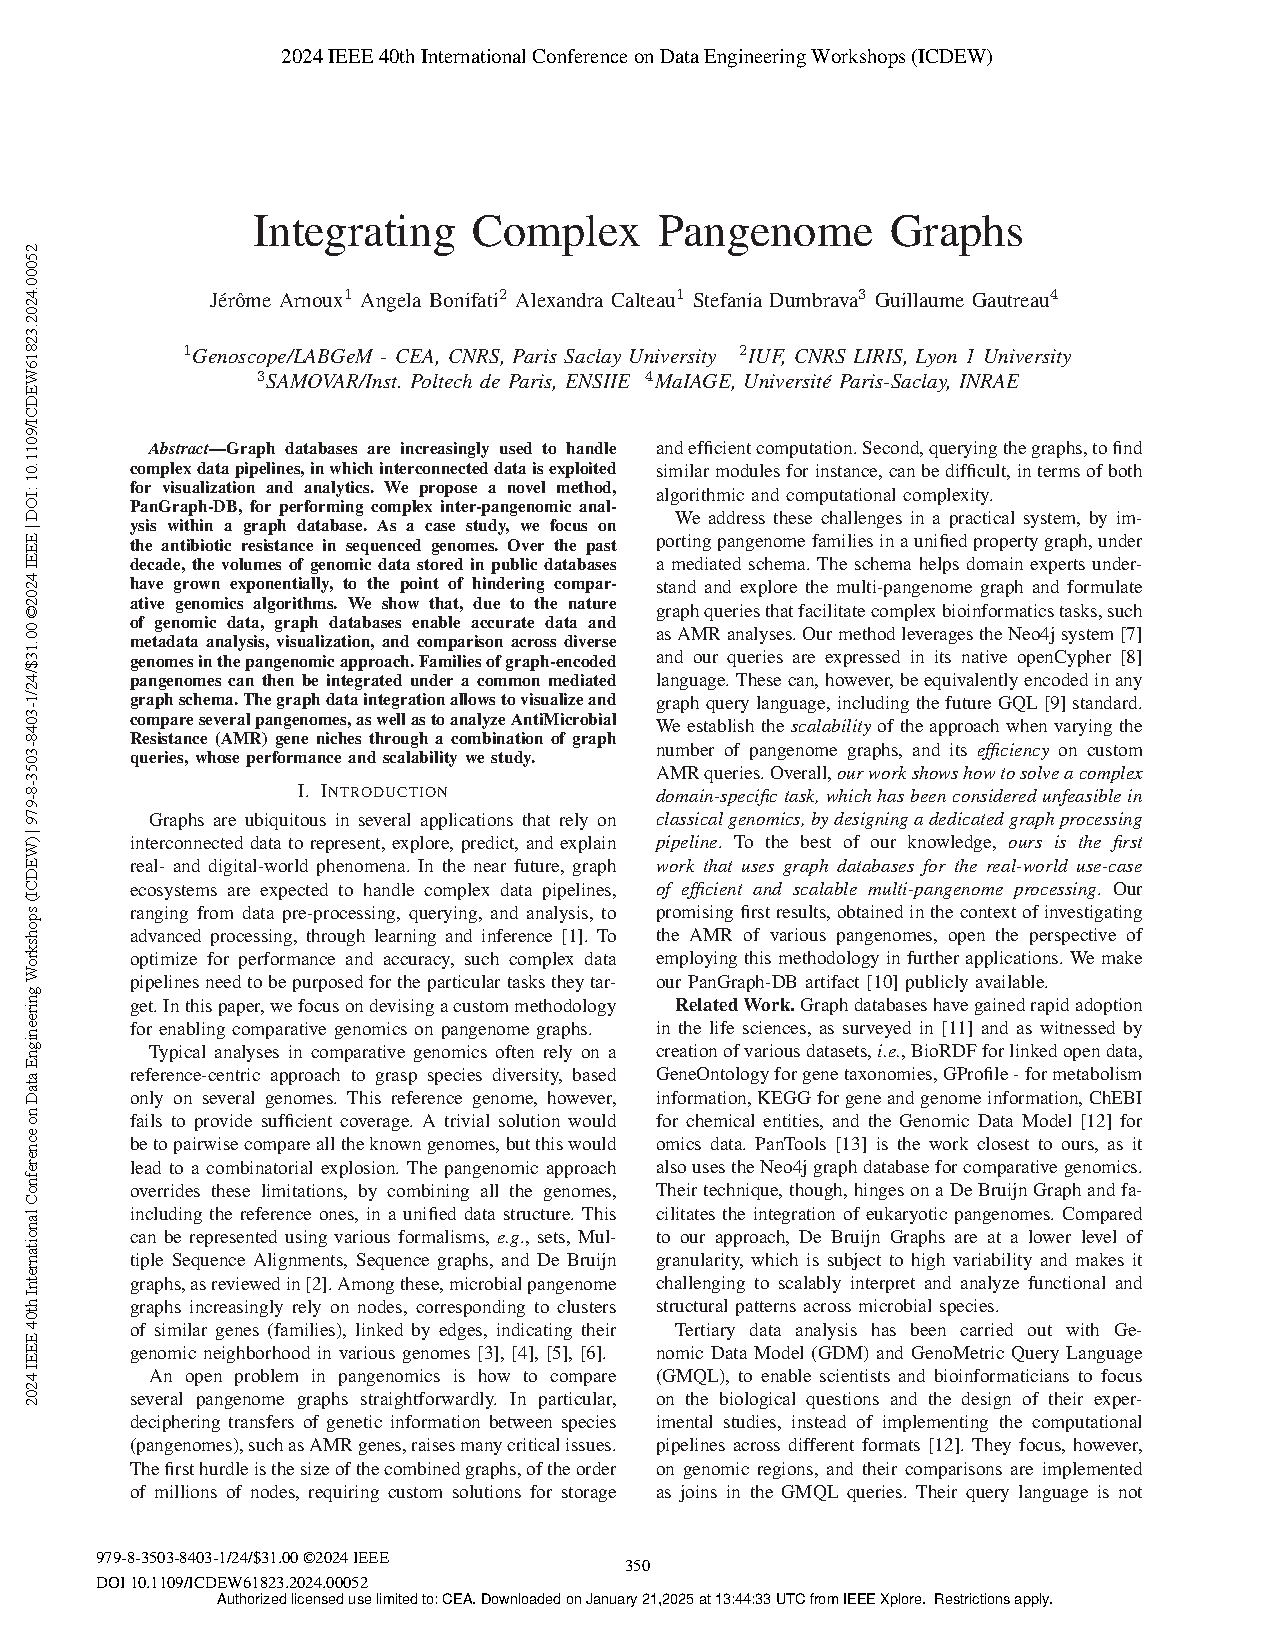
\includepdf[pages=-]{GraphDataBase/Integrating_Complex_Pangenome_Graphs.pdf}

\chapter{Conclusion et perspectives}

Notre \textit{proof of concept} sur l'intégration et l'analyse de pangénomes dans des bases de données orientées graphe, ouvre la voie à de nouvelles méthodes de stockage, d’analyse et de visualisation de vastes ensembles de génomes et de pangénomes. Nous avons conçu un schéma de base de données ainsi qu’un workflow d’analyse générique, pouvant être adaptés à d'autres modèles de pangénomes. Nos tests montrent que notre approche permet des temps de réponse très rapides (de l’ordre de la milliseconde) aussi bien pour des requêtes simples que pour des analyses complexes. Bien que notre POC soit une réussite, plusieurs améliorations sont nécessaires pour en faire une véritable base de données opérationnelle dédiée à l’analyse et à la distribution des pangénomes.

Pour intégrer les pangénomes dans la base de données, j'ai développé un script Python utilisant \textbf{PPanGGOLiN} et \textbf{PANORAMA} afin d’extraire et de préparer les données. L’intégration dans Neo4j s’est appuyée sur des packages tiers, non optimisés pour nos données, entraînant des temps d’intégration relativement longs. Récemment, Neo4j a publié un package officiel, plus flexible et optimisé pour la communication avec la base. Les premiers tests, que j'ai menés, indiquent qu’il permettrait une réduction significative des temps d’intégration, ce qui constitue une piste prometteuse pour améliorer l'efficacité globale du système.

Lors d’un second hackathon D4GEN en 2023, l’intégration de \textbf{méthodes de machine learning} a été explorée dans notre workflow d’analyse. Neo4j propose plusieurs packages dédiés à l’application du ML directement sur la base de données. Nous avons testé différentes approches pour identifier des structures et des chemins pertinents dans le graphe de pangénome, mais aucun résultat probant n’a émergé.
Cependant, cette première tentative nous a permis de repenser le schéma de la base de données et d'imaginer de \textbf{nouvelles métadonnées} à intégrer pour des analyses futures.

Pour construire la BD Neo4J, j'ai développé un script permettant de charger les pangénomes dans une base de données locale. Ce script avait d'abord été intégré à PANORAMA, pour sa capacité à lire plusieurs pangénomes. Toutefois, nous avons finalement choisi de développer un script indépendant, plus facile à maintenir. Ce script offre plusieurs avantages : intégration simplifiée des pangénomes dans la base, lancement automatique des analyses, indépendance vis-à-vis de l’interface Neo4j.
L’objectif étant de rendre l’ensemble du processus plus accessible et automatisé, afin que chacun puisse créer une instance propre de base de données de pangénomes.

Le \textbf{LABGeM} développe une base de données de pangénomes générés par PPanGGOLiN, \textbf{PanGBank}. Ce projet repose sur une architecture de BD relationnelle \textbf{SQL}, contenant les fichiers \textbf{HDF5} pour chaque espèce et des résultats d’analyse accessibles en ligne.
Une intégration avec notre POC pourrait offrir plusieurs avantages :
\begin{itemize}
    \item Une \textbf{nouvelle manière d’organiser et de visualiser les pangénomes}
    \item La possibilité d’\textbf{effectuer des analyses complexes directement sur la base de données}
    \item Une meilleure interconnexion entre les données et les outils d’exploration
\end{itemize}
En combinant ces approches, nous pourrions développer un système de gestion des pangénomes plus robuste, interactif et performant.


\addcontentsline{toc}{part}{\nameBib}
\bibliographystyle{apalike-fr}
\bibliography{References/references}
\end{document}